\label{res}
This chapter presents the results of the tests described in \autoref{s20},  \ref{het-test-meth}, and  \ref{meth-sens}.  Section \ref{res-comps} first presents the atomic fractions of select isotopes of interest, and the fission rate/thermal flux mesh corresponding to each depletion time step.  Then, \autoref{res-control} covers the results of the basic control model. The final sections --- dedicated to homogenization (see \autoref{res-hom}), symmetry (see \autoref{res-sym}), and shuffling (see \autoref{res-shuff}) --- compare the results of these perturbations to the control model.

\section{Fuel Isotopic Compositions}
\label{res-comps}

Figure \ref{fig:burn-meshes} depicts the evolution of the fission rate (hot color map) and thermal flux (cold color map) over the seven stages of burnup that we chose to model.  The maximum cutoff for thermal flux is 0.625 eV in these figures.  Over successive depletion steps, the fission rate and thermal flux increases.  This is not unexpected --- as the pebble burns, the atomic fraction of fissile $^{235}U$ decreases.  This requires that the fission rate increase to maintain criticality.  Notably, the fission rate mesh for the six-month depletion step has fewer points indicating higher values when compared to the initial depletion step; however, the scales of these images are not uniform, and this is likely indicative of the fission rate profile within the six-pass pebble flattening.

\begin{figure}[H]
\centering
%
\begin{subfigure}{0.4\textwidth}
  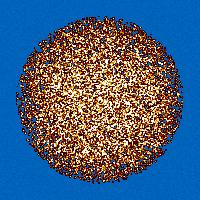
\includegraphics[width=0.95\linewidth]{figures/burn-20-bstep0}
  \caption{Fresh}
  \label{fig:bstep0}
\end{subfigure}%
%
\begin{subfigure}{0.4\textwidth}
  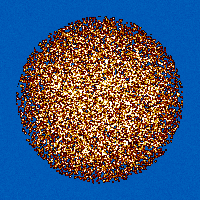
\includegraphics[width=0.95\linewidth]{figures/burn-20-bstep1}
  \caption{One Pass}
  \label{fig:bstep1}
\end{subfigure}%

\caption{Mesh Figures For Single Pebble Burnup}
\end{figure}

\begin{figure}[H]\ContinuedFloat
\centering

\begin{subfigure}{0.4\textwidth}
  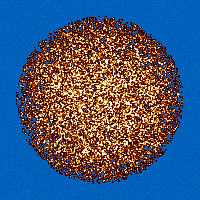
\includegraphics[width=0.95\linewidth]{figures/burn-20-bstep2}
  \caption{Two Passes}
  \label{fig:bstep2}
\end{subfigure}%
%
\begin{subfigure}{0.4\textwidth}
  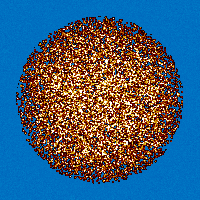
\includegraphics[width=0.95\linewidth]{figures/burn-20-bstep3}
  \caption{Three Passes}
  \label{fig:bstep3}
\end{subfigure}%

\begin{subfigure}{0.4\textwidth}
  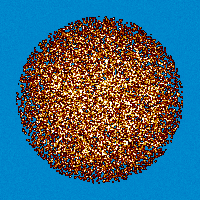
\includegraphics[width=0.95\linewidth]{figures/burn-20-bstep4}
  \caption{Four Passes}
  \label{fig:bstep4}
\end{subfigure}%
%
\begin{subfigure}{0.4\textwidth}
  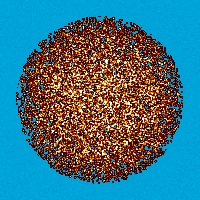
\includegraphics[width=0.95\linewidth]{figures/burn-20-bstep5}
  \caption{Five Passes}
  \label{fig:bstep5}
\end{subfigure}%

\begin{subfigure}{0.4\textwidth}
  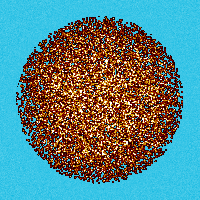
\includegraphics[width=0.95\linewidth]{figures/burn-20-bstep6}
  \caption{Six Passes}
  \label{fig:bstep6}
\end{subfigure}%
%
\caption{Mesh Figures For Single Pebble Burnup(cont.)}
\label{fig:burn-meshes}
\end{figure}

Understanding the effects on core neutronics such as the fission rate or thermal flux is not the only reason to find the isotopic composition of the fuel.  Fission product buildup in the fuel has long term ramifications for spent fuel handling, and matters for our understanding of accident consequence analysis.  The potential isotopes --- and in what amounts --- that a living being or environment might be exposed to after an accident is called a source term.  As shown in Tables \ref{table:gas-acc} and \ref{table:dust-acc} in Chapter 1, fission products can either leach into the coolant gas, or be found in the fine dust formed when the pebbles bump against each other during operation.  In an accident, this dust could end up outside of the \acrshort{rpv} in the case of a breach, where it could be inhaled or reach the ground or groundwater.  In order to fully understand accident consequences, one must robustly characterize the source term.  Figure \ref{fig:comps} provides the atomic fractions of isotopes of iodine, xenon, cesium, uranium, and plutonium within depleted fuel in the Sangamon Reactors.

\begin{figure}[H]
\centering
%
\begin{subfigure}{0.8\textwidth}
  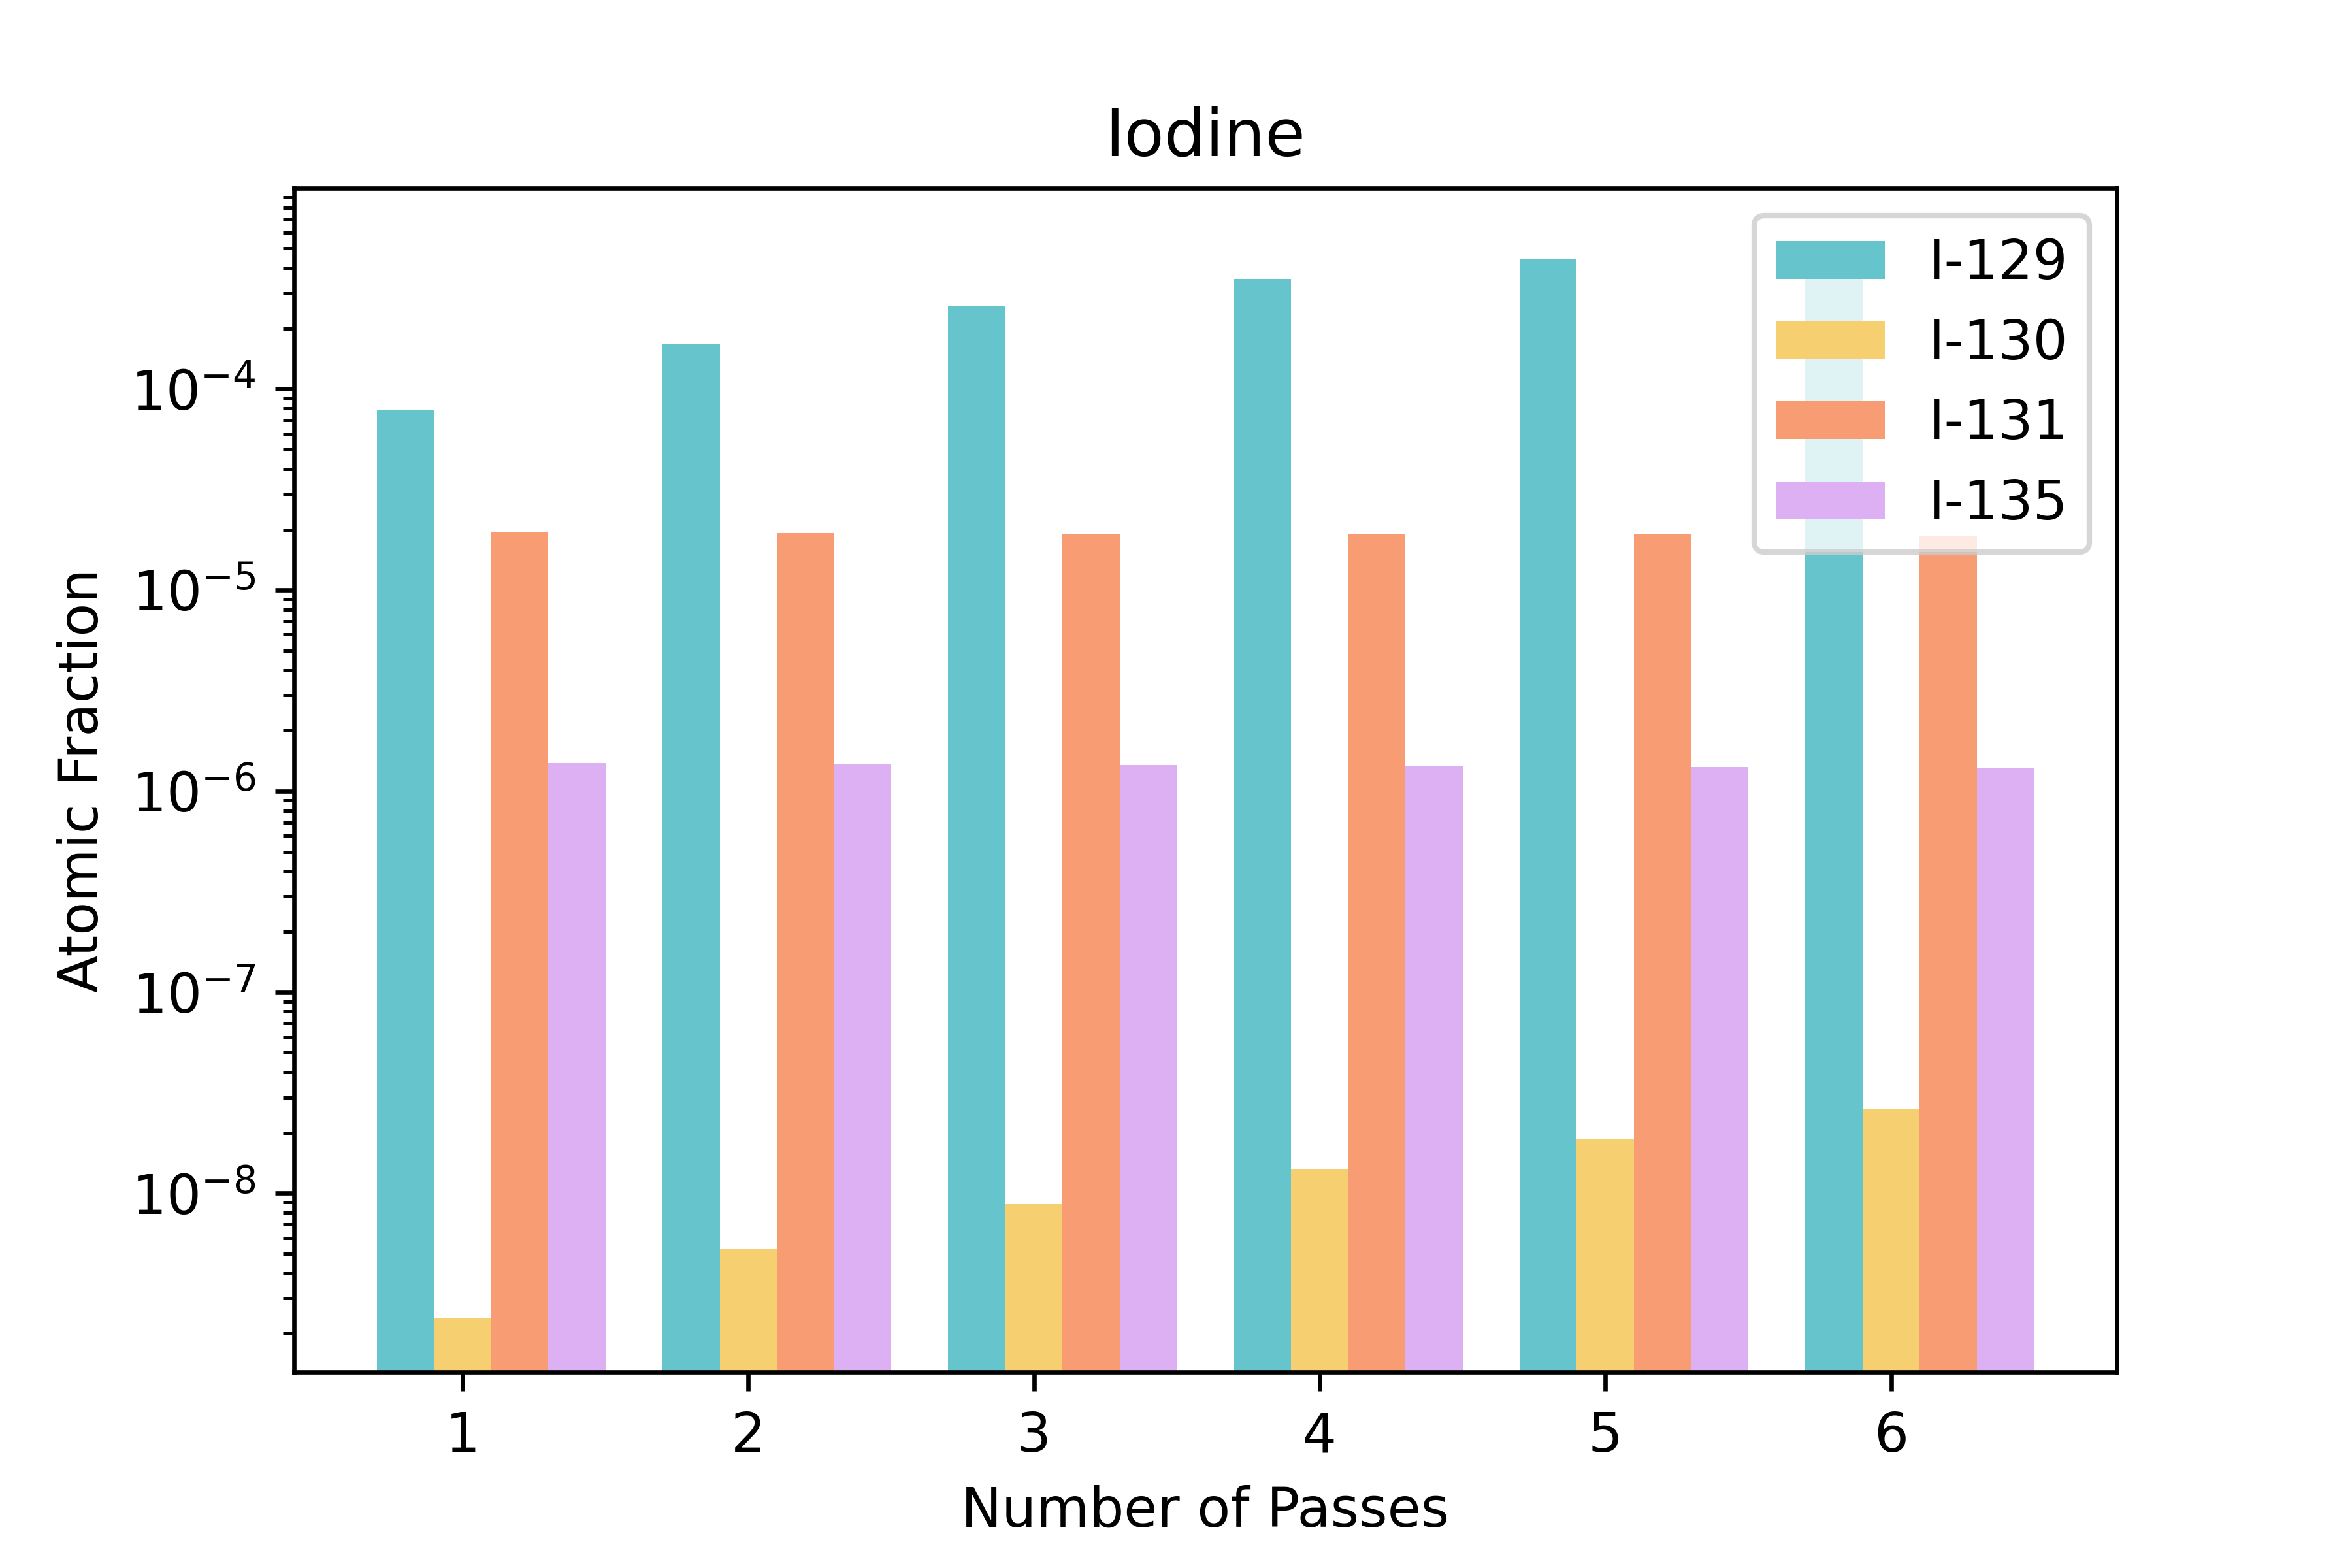
\includegraphics[width=\linewidth]{figures/compositions/iodine}
  \caption{Iodine isotope buildup over six burnup stages}
  \label{fig:i}
\end{subfigure}%

\begin{subfigure}{0.8\textwidth}
  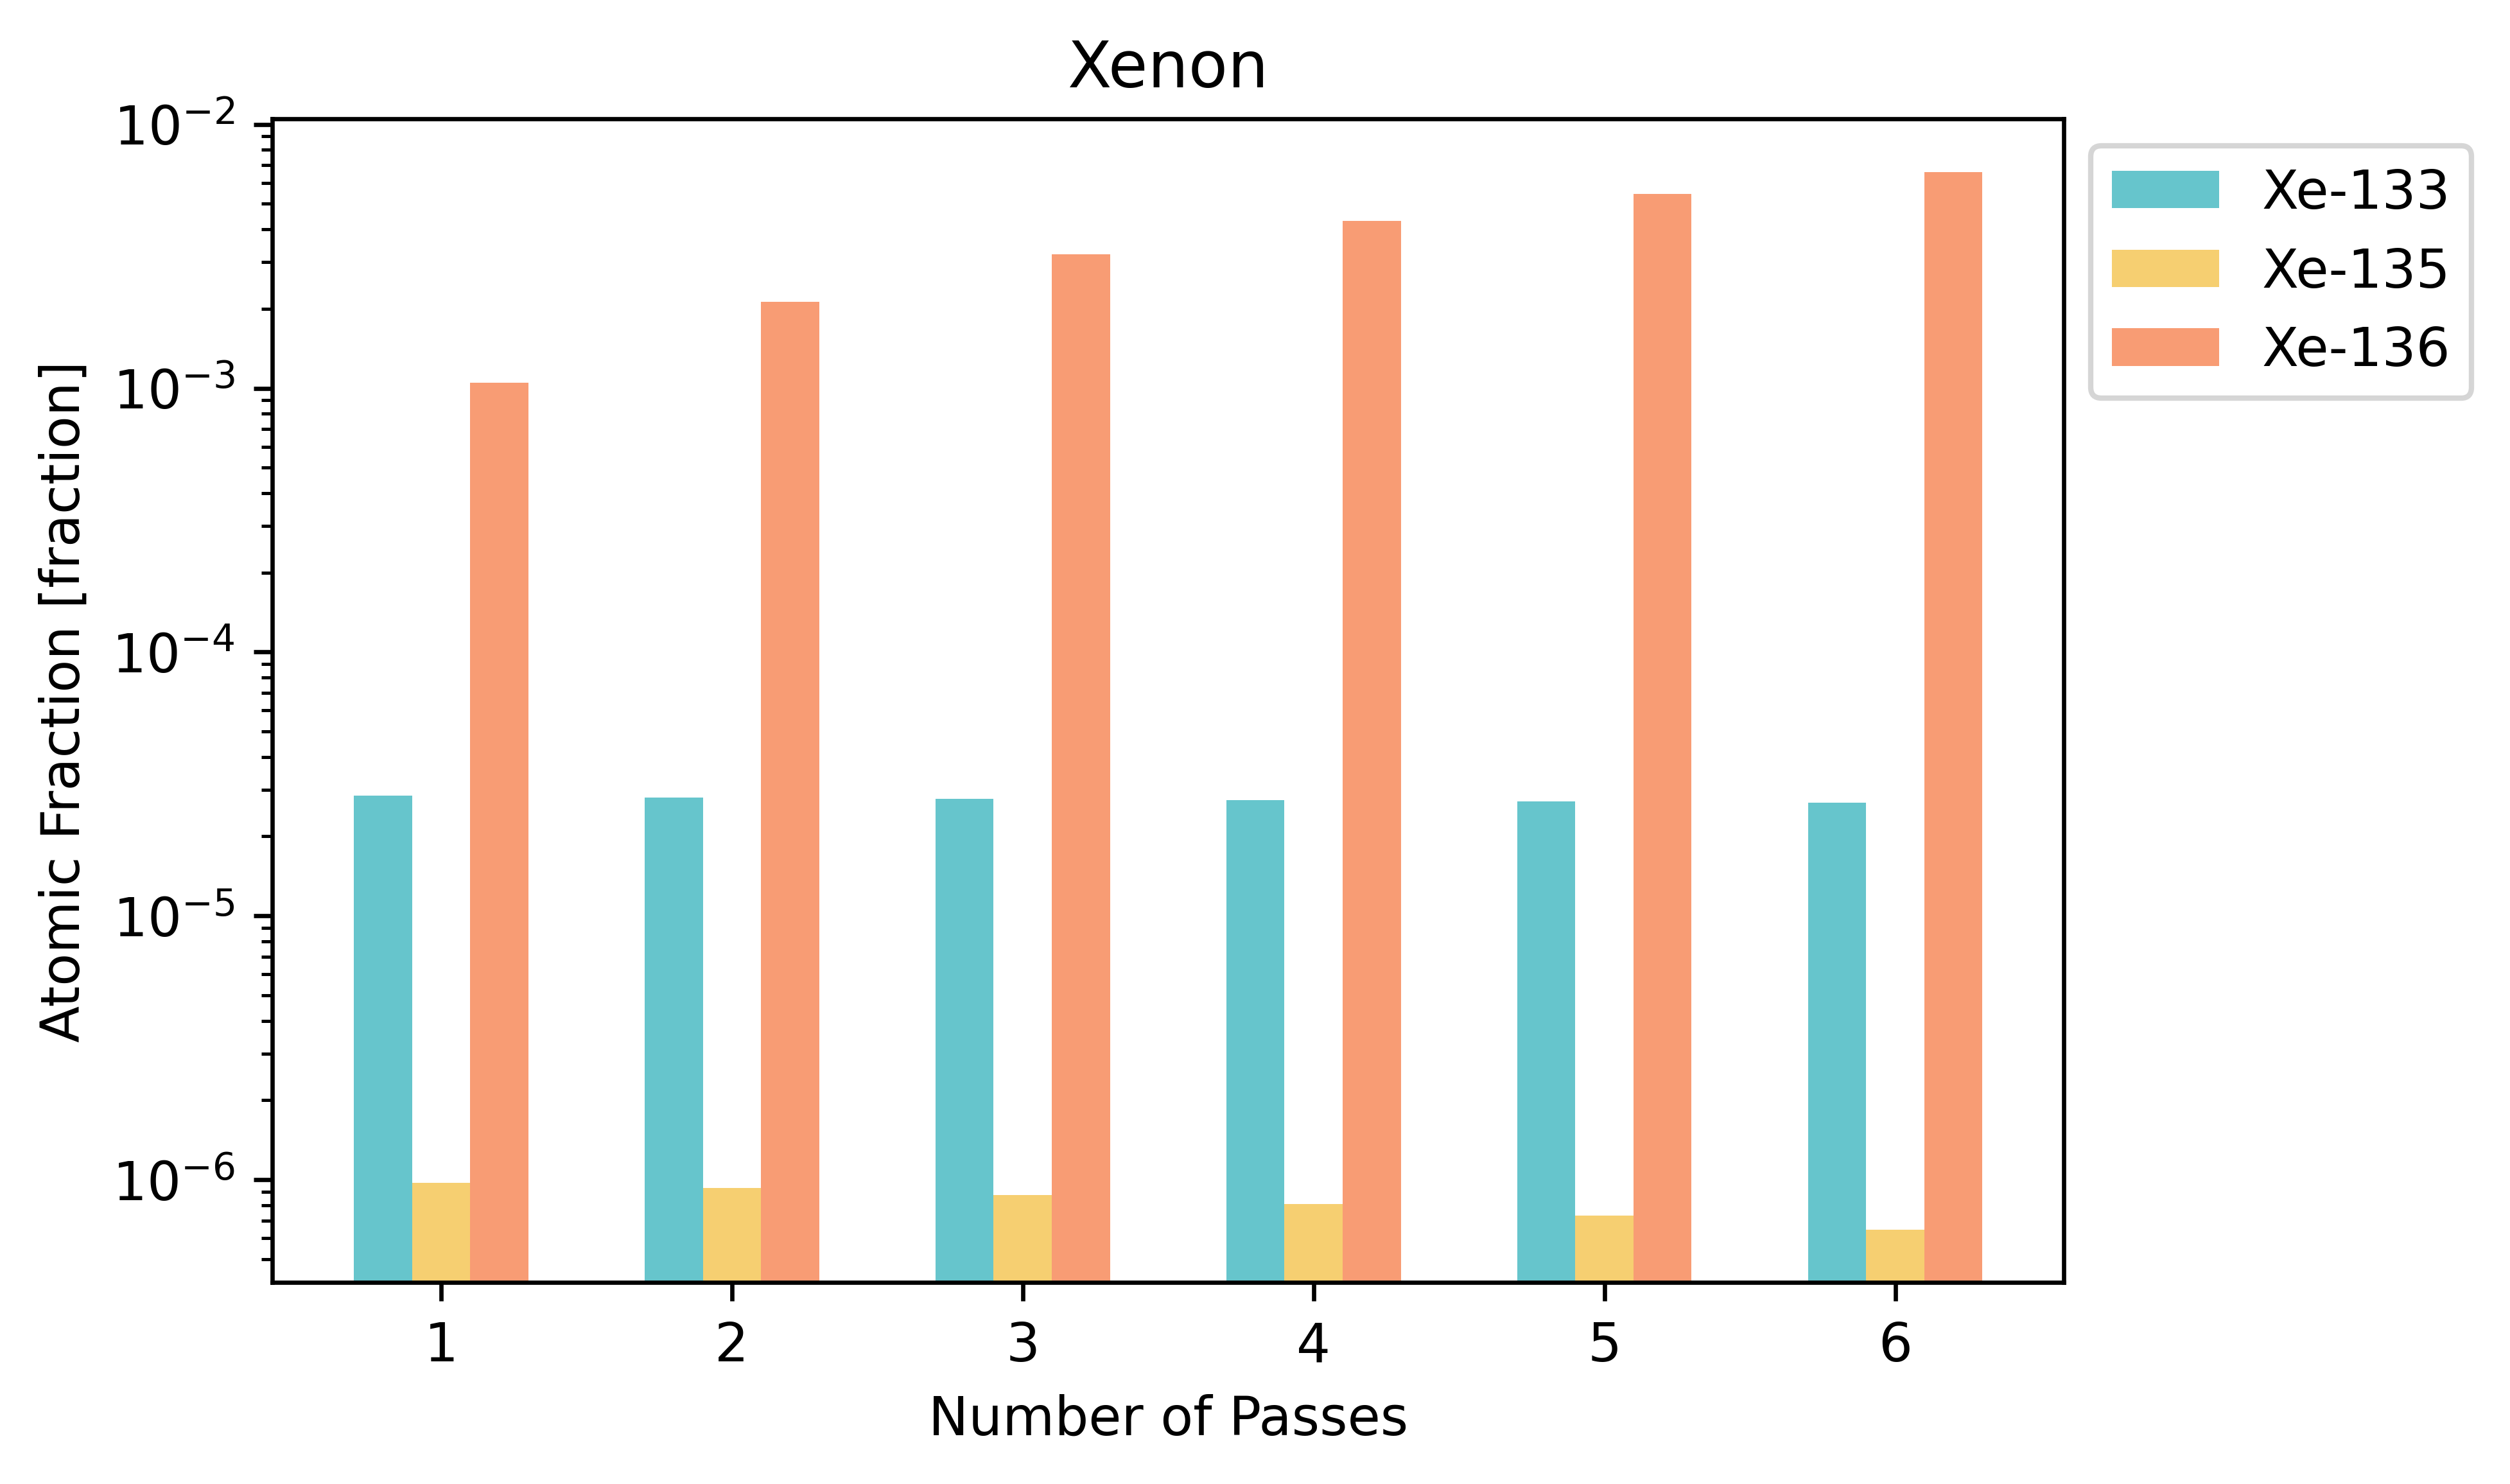
\includegraphics[width=\linewidth]{figures/compositions/xenon}
  \caption{Xenon isotope buildup over six burnup stages}
  \label{fig:xe}
\end{subfigure}%

\caption[Evolution of Safety Relevant Isotopic Concentrations in Pebbles of Sangamon20 over Six Six-Month Passes]{Evolution of Safety Relevant Isotopic Concentrations in Pebbles of Sangamon20 over Six Six-Month Passes (measured in atomic fraction)}
\end{figure}

\begin{figure}[H]\ContinuedFloat
\centering

\begin{subfigure}{0.8\textwidth}
  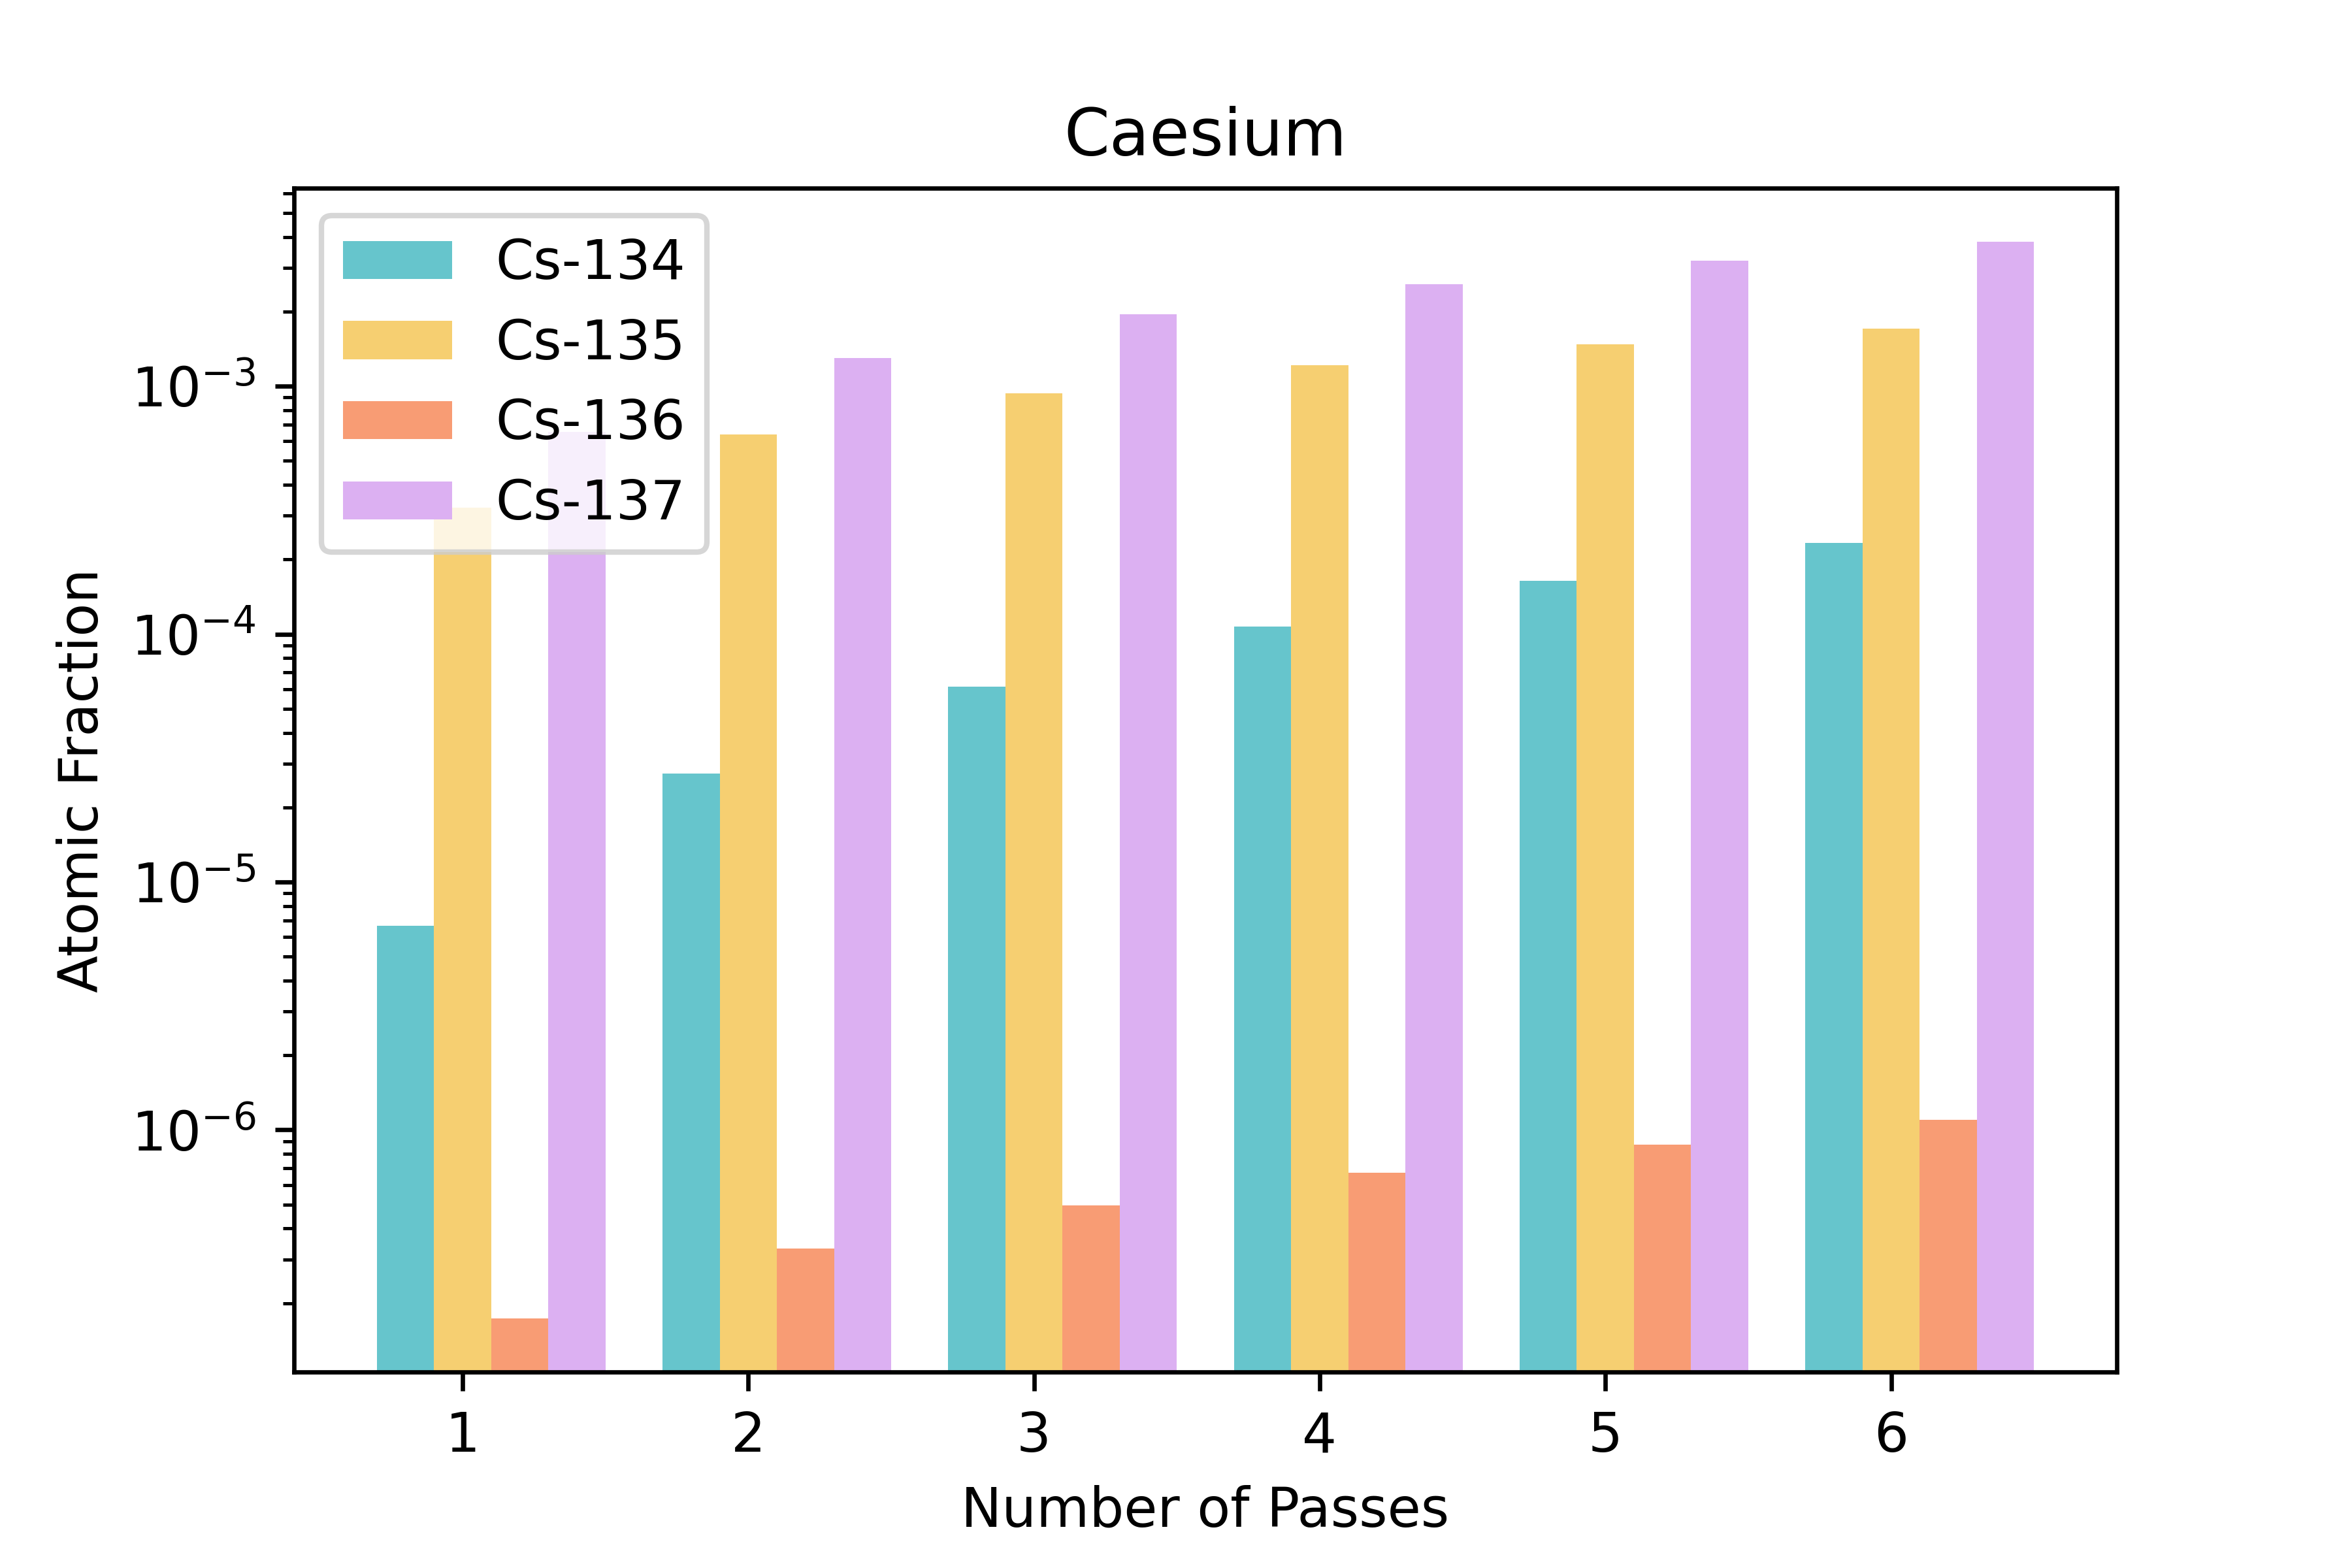
\includegraphics[width=\linewidth]{figures/compositions/caesium}
  \caption{Cesium isotope buildup over six burnup stages}
  \label{fig:cs}
\end{subfigure}%


\begin{subfigure}{0.8\textwidth}
  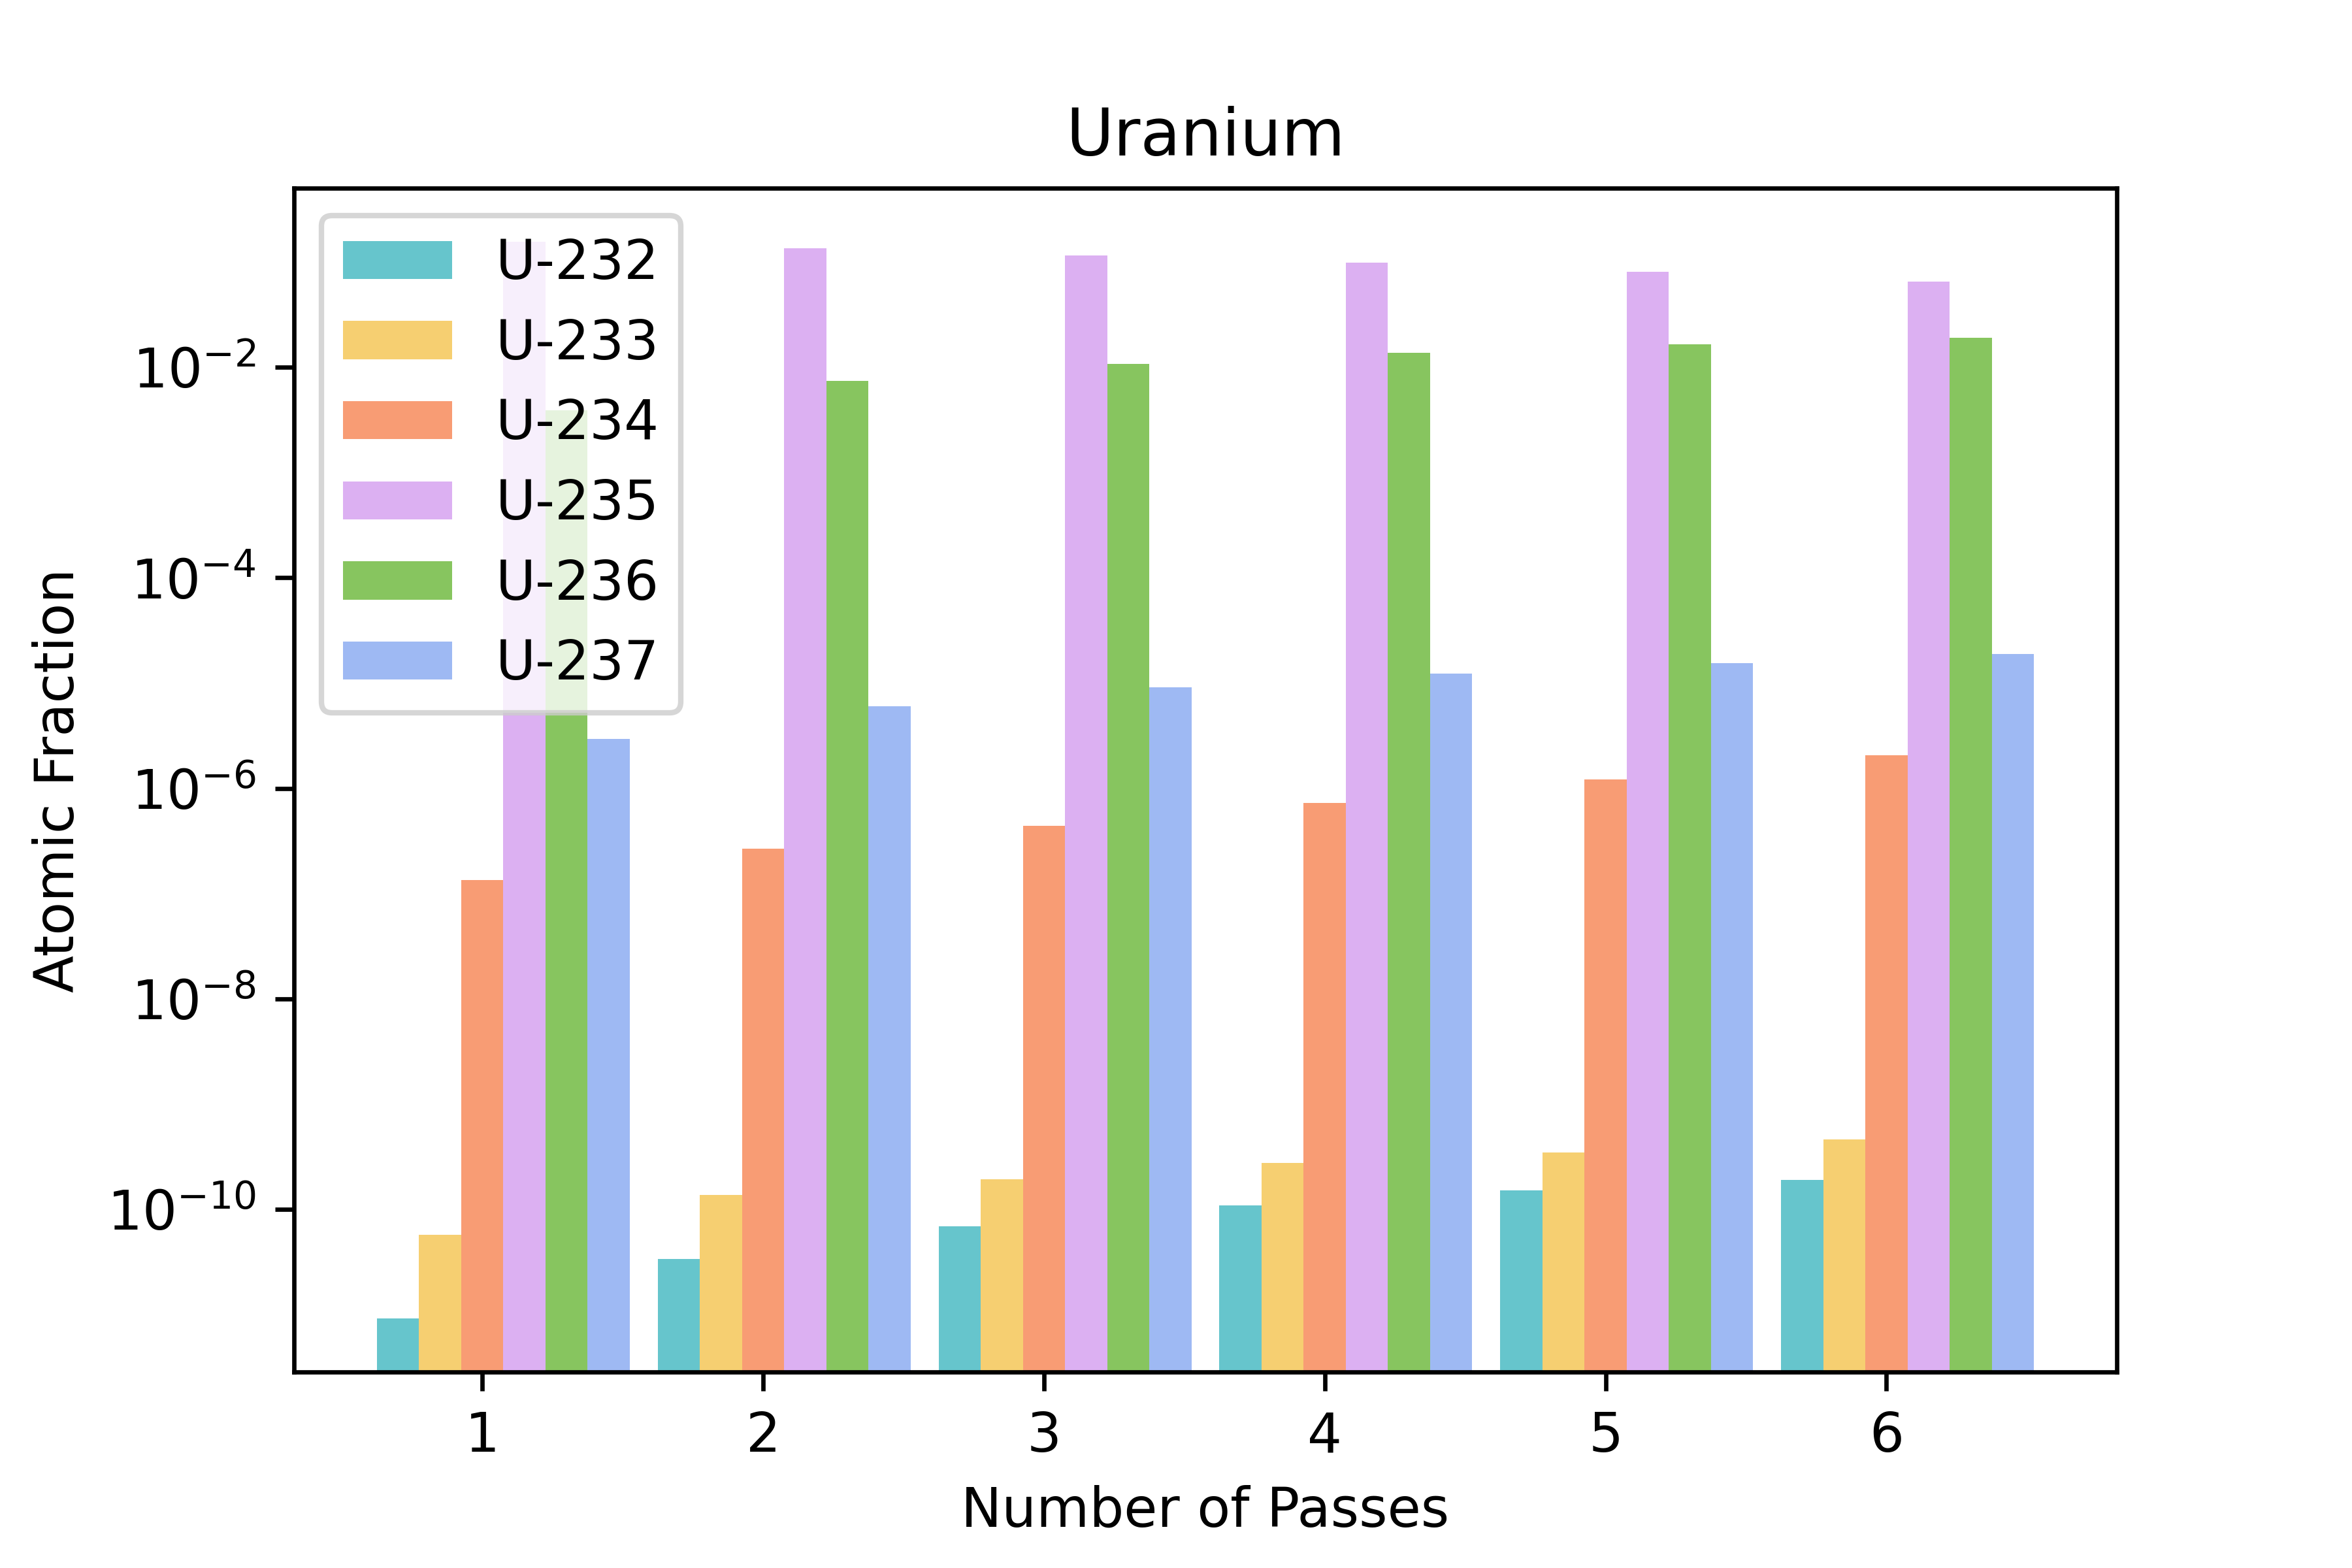
\includegraphics[width=\linewidth]{figures/compositions/uranium}
  \caption{Uranium isotope buildup over six burnup stages}
  \label{fig:u}
\end{subfigure}%

\caption[]{(cont.)}
\end{figure}

\begin{figure}[H]\ContinuedFloat
\centering

\begin{subfigure}{0.8\textwidth}
  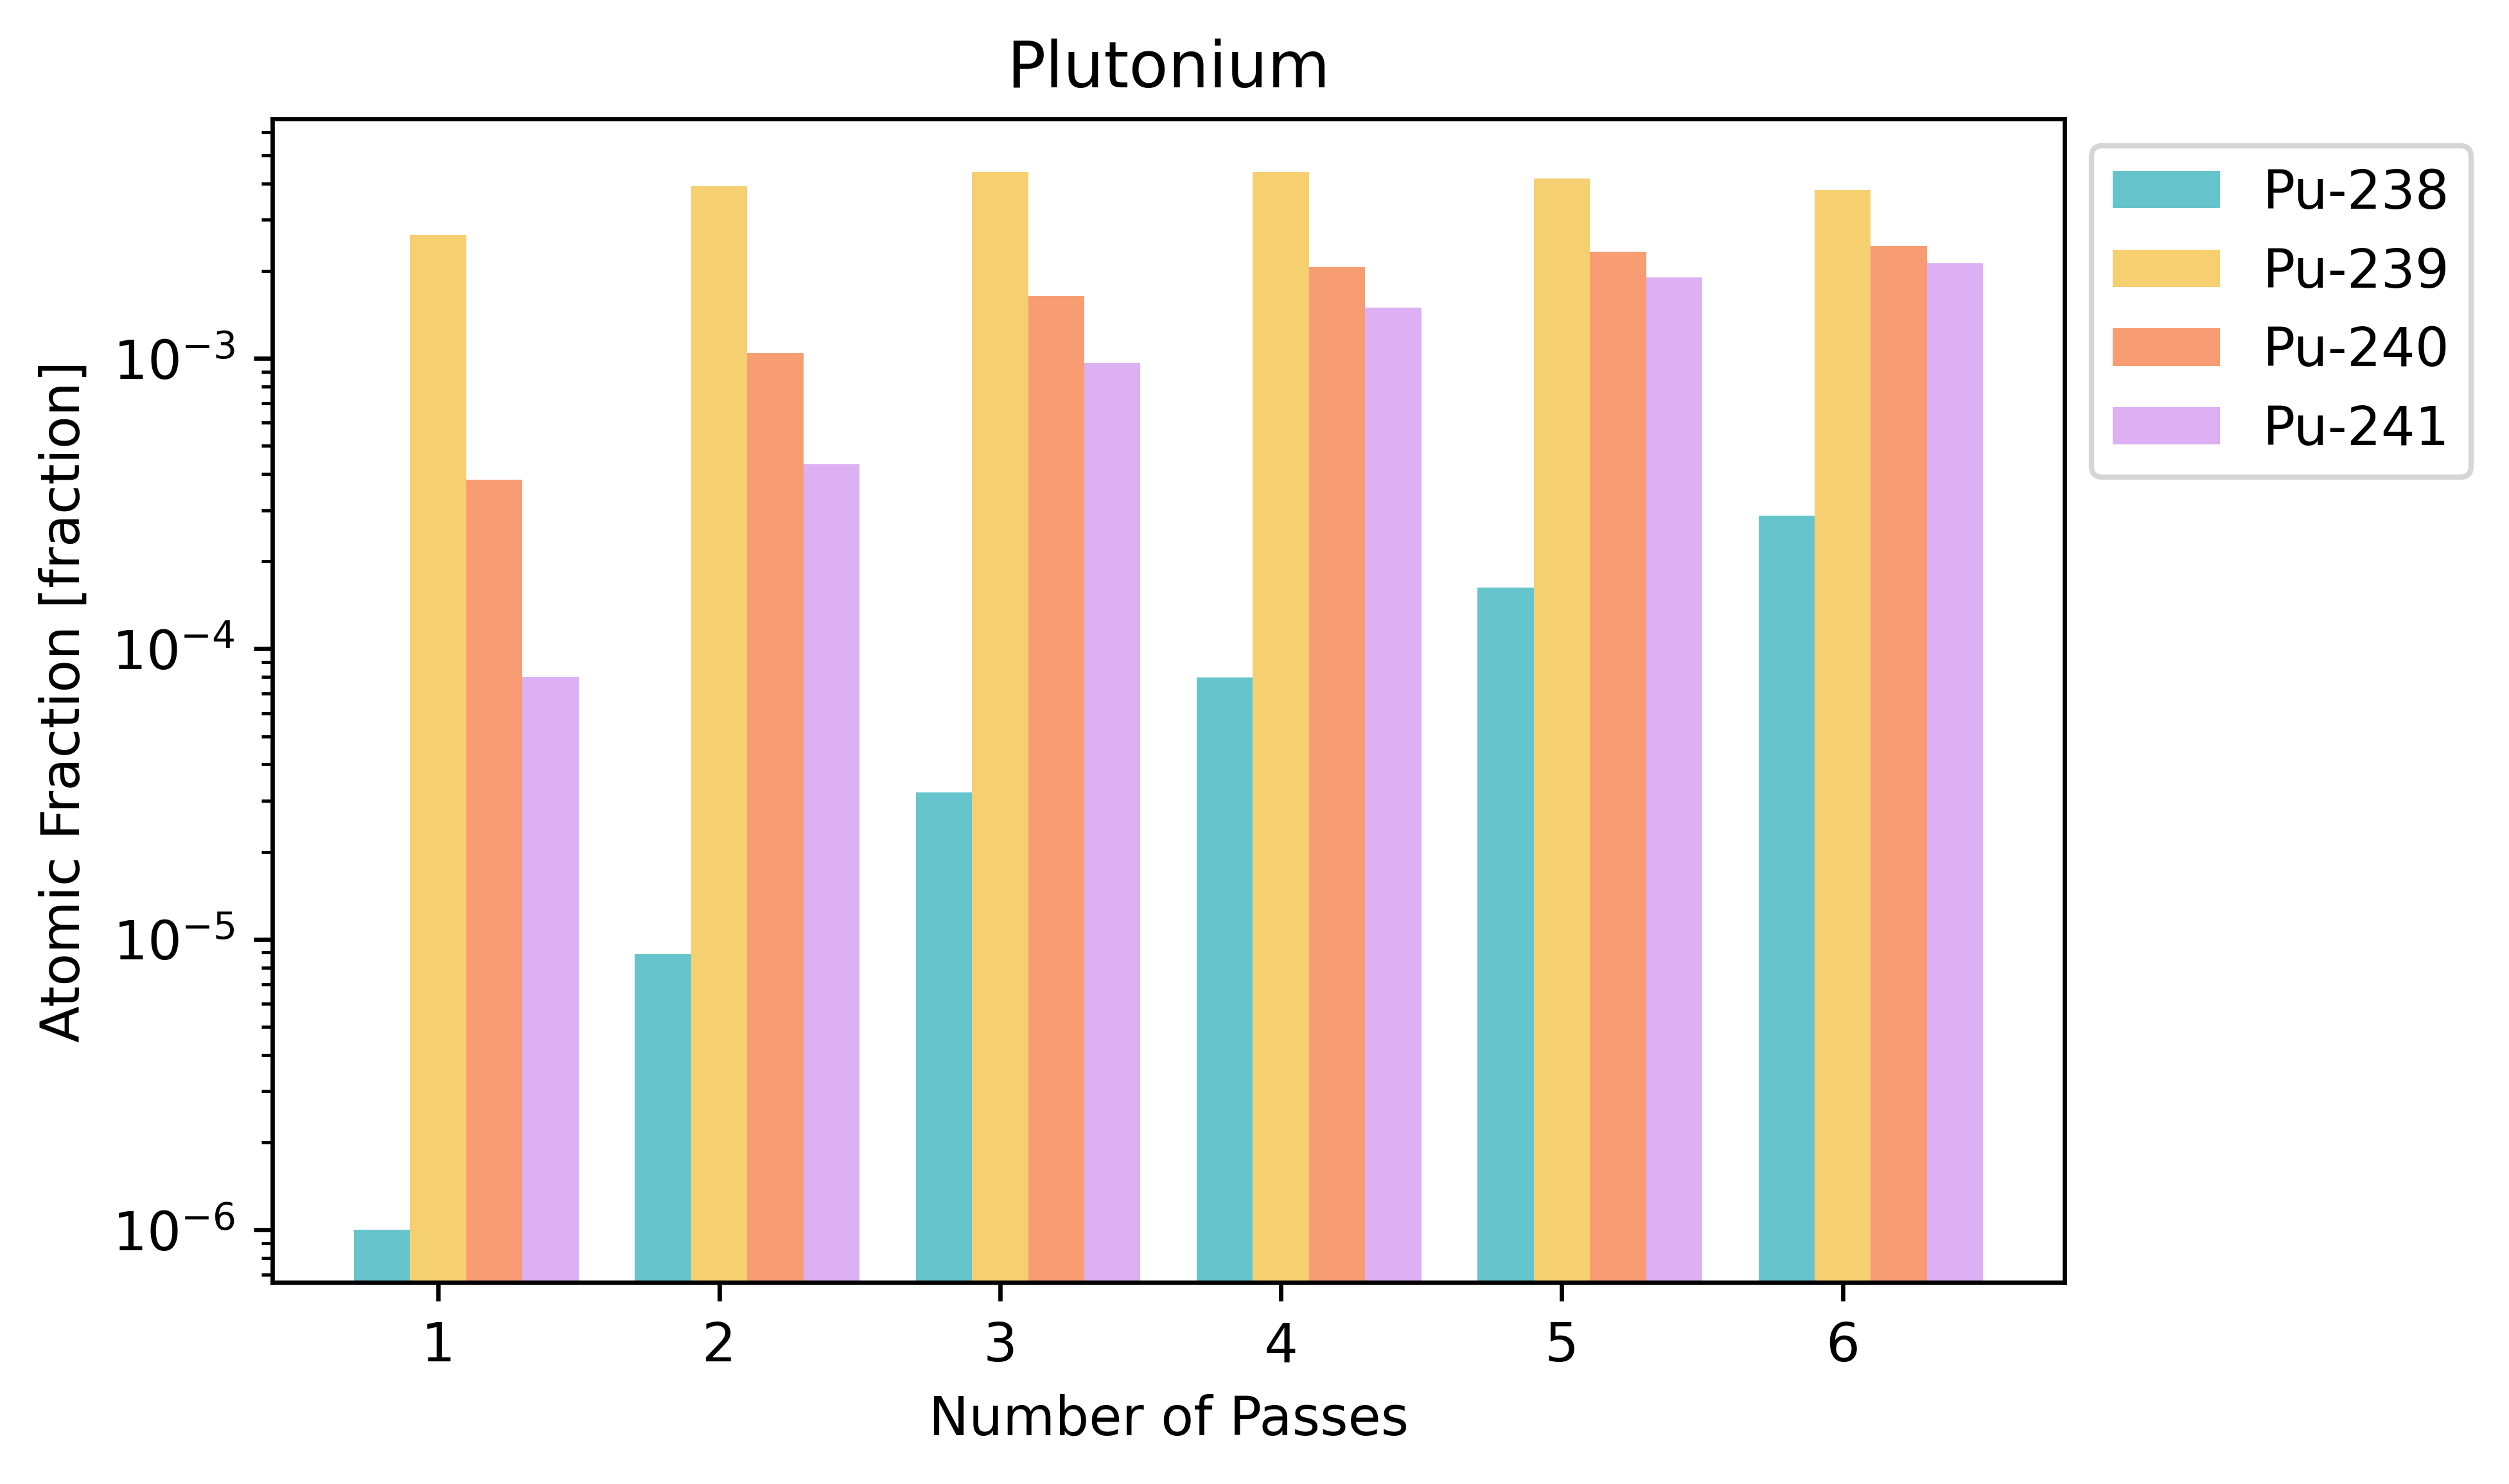
\includegraphics[width=\linewidth]{figures/compositions/plutonium}
  \caption{Plutonium isotope buildup over six burnup stages}
  \label{fig:pu}
\end{subfigure}%

\caption[]{(cont.)}
\label{fig:comps}
\end{figure}

The full isotopic inventory tracked in the Sangamon20 reactor models extends far beyond those supplied in Figure \ref{fig:comps}.  For a full list, see \cite{richter_isotopic_2021} and \cite{richter_isotopic_2022} for the compositions in Sangamon20 and Sangamon200, respectively, or \cite{richter_zoerichterphlox_2022} for a complete input file and associated output.  Figure \ref{fig:comps} focuses on those of interest in safety analysis, such as those in Table \ref{table:dust-acc} and Table \ref{table:gas-acc}.

All isotopes of uranium steadily increase over time with the exception of $^{235}U$, ending at 0.0647 by atomic fraction in the sixth pass --- significantly lower than the 0.17698 it started with.  $^{232}U$, initially the smallest fraction of uranium sees the most dramatic increase over time, increasing by two orders of magnitude between the first ($9.28\times10^{-12}$) and sixth ($1.9\times10^{-10}$) cycle.  While the atomic fraction doesn't reach an equilibrium, the rate at which it increases each cycle is steady by the third pass - increasing by $4.02\times10^{-11}$,$4.2\times10^{-11}$, and $3.9\times10^{-11}$ from the third to fourth, fourth to fifth, and fifth to sixth pass, respectively.  The behavior of plutonium is also of interest, with $^{239}Pu$ peaking at 0.00439.  However, unlike many other isotopes, which peak in the sixth cycle, $^{239}Pu$ crests in the third and fourth passes, decreasing from 0.00439 in the fourth pass to 0.00380 in the sixth as it begins to burn away.  $^{238}Pu$, meanwhile, is the least abundant, but does experience the most dramatic increase over time (especially between the first and second passes).



Only the xenon content rivals the inventory of uranium.  $^{133}Xe$ appears to be steady around its initial concentration of $2.86\times10^{-05}$ atomic fraction, decreasing only to $2.68\times10^{-05}$ by the sixth pass.  $^{135}Xe$ is mostly stable, but does decrease slightly over the full residence time of the pebble, going from an initial $9.70\times10^{-07}$ after its first six months, to  $6.46\times10^{-07}$ after thirty-six months.  $^{136}Xe$ is both the greatest contributor to xenon content in the fuel, and the only isotope reported in  Figure \ref{fig:xe} to increase, owing to its long half life.  Each cycle increases $^{136}Xe$ content by ~0.0011, beginning at a concentration of 0.00105 in the first cycle and ending at 0.0066 after the sixth.  Isotopes of iodine form a smaller portion of fission products than xenon or cesium (still a relatively high magnitude) which is of concern due to its high mobility in water and uptake in the thyroid.  $^{129}I$ is the most abundant isotope of iodine reported here.  It increases for the entirety of the pebble's life, beginning at $7.38\times10^{-05}$ and peaking at 0.000538 at its discharge burnup.  $^{130}I$ and $^{135}I$ are both relatively stable, due to their short half-lives, combined with transmutation after undergoing neutron capture.  While $^{130}I$ is the least abundant, it increases over time.  Cesium has a net concentration similar to xenon's.  Unsurprisingly $^{135}Cs$ and $^{137}Cs$, which both have half-lives longer than a pebble's residency time in the reactor, are in greatest abundance, and increase over time.  These, too, are of concern, due to their long half-life.

\section{Full-Core Control Model}
\label{res-control}

The control model of the Sangamon20 reactor is the basis for the three characterization tests this work performed, and it is the model that the results of these tests are compared against.  Figure \ref{fig:controlmain} shows a cross section of the core geometry at the origin (the midplane, the center of which is the point (0, 0, 0) ) in the xy and xz planes (Sub-Figures \ref{fig:controla} and \ref{fig:controlc}, respectively) and provides a mesh of the fission rate and thermal flux in the xy and xz planes (Sub-Figures \ref{fig:controlb} and \ref{fig:controld}, respectively).  Both of these integrate over z and y, respectively, to produce a 2D image.  The value of $k_{eff}$ is $1.009 \pm 0.00055$, while the outward neutron current at the reflector edge is $7.003\times 10^{11} \pm 8.683\times 10^{08}$.

Figure \ref{fig:geom-legend1} is a legend of material compositions in all cross-sectional geometry figures.  In homogenized simulations, the shades of green represent the material blend forming the center of the pebble at a given burnup.  For heterogenized simulations, these same shades represent the TRISO particle kernel at a particular burnup.

\begin{figure}[H]
\centering

\begin{subfigure}{0.45\textwidth}
  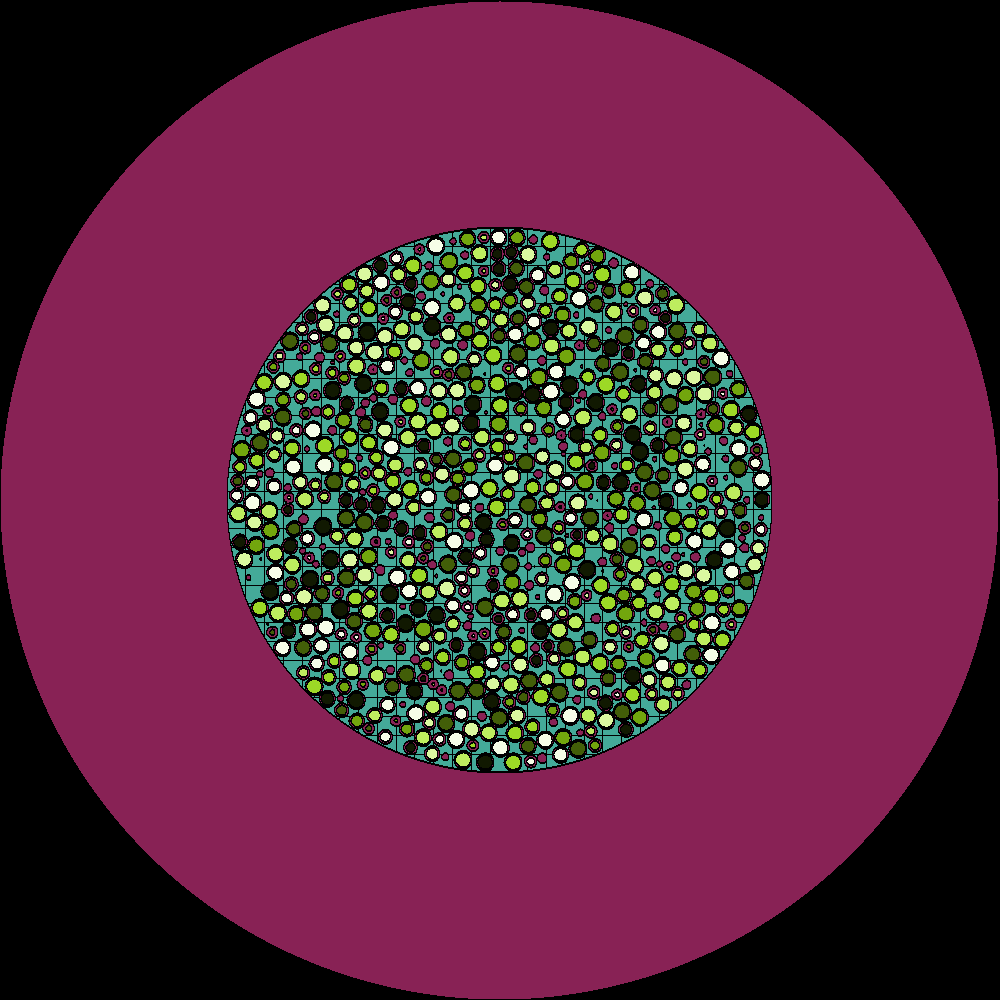
\includegraphics[width=0.95\linewidth]{figures/control/control-r}
  \caption{Radial Cross Section at y=0}
  \label{fig:controla}
\end{subfigure}%
%
\begin{subfigure}{0.45\textwidth}
  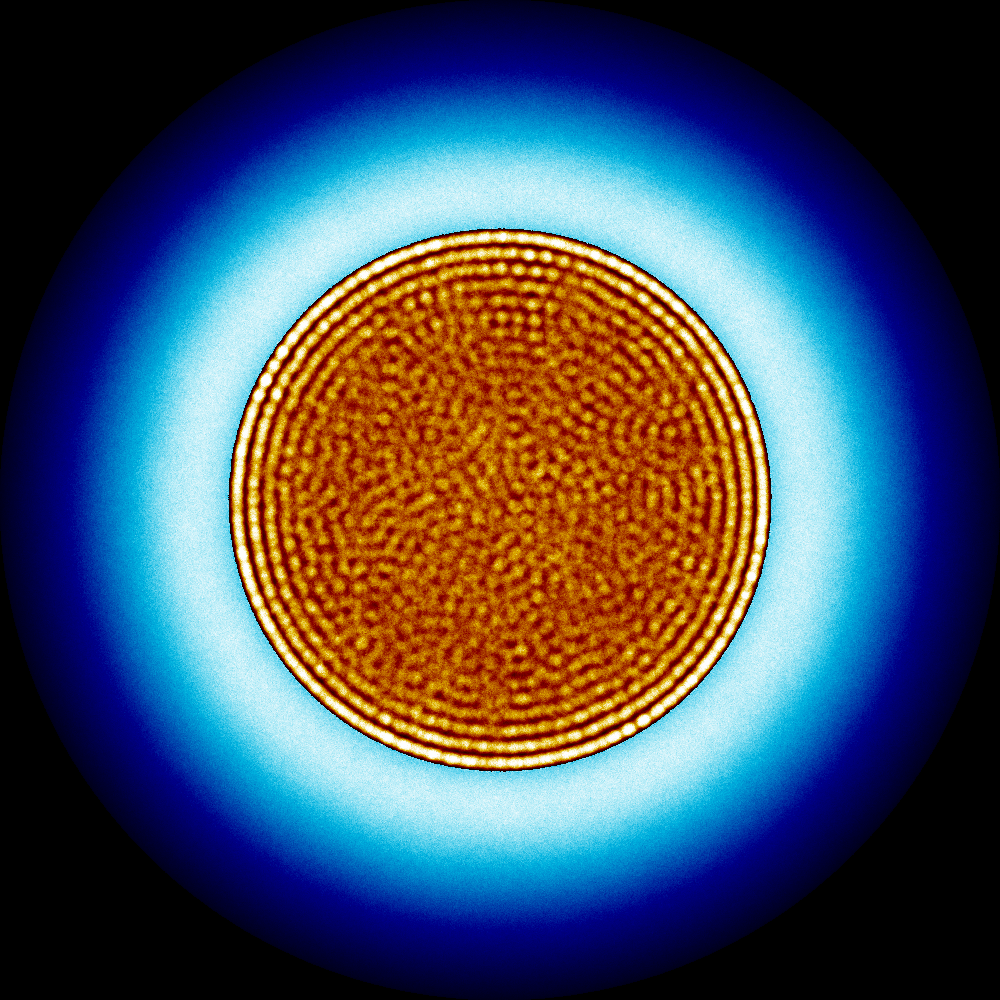
\includegraphics[width=0.95\linewidth]{figures/control/control-rm}
  \caption{Radial Mesh}
  \label{fig:controlb}
\end{subfigure}

\begin{subfigure}{0.45\textwidth}
  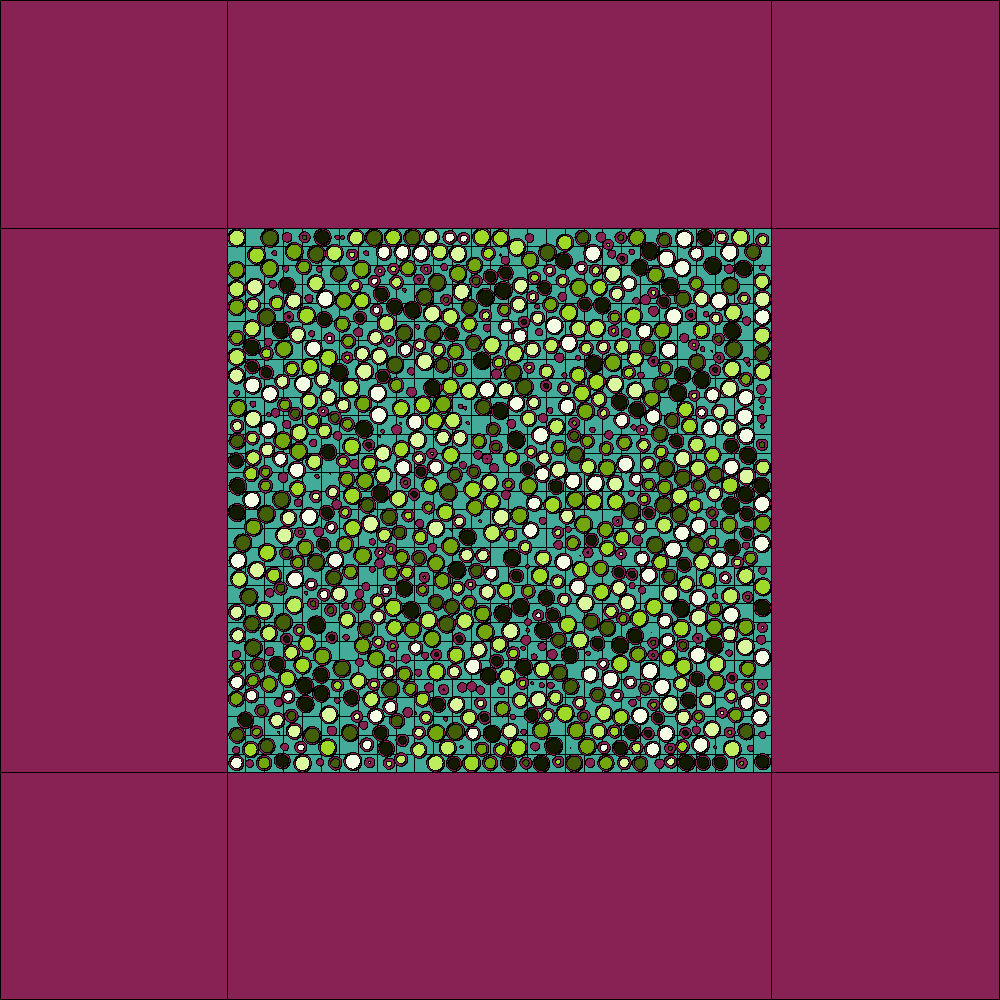
\includegraphics[width=0.95\linewidth]{figures/control/control-v}
  \caption{Axial Cross Section at z=0 }
  \label{fig:controlc}
\end{subfigure}
%
\begin{subfigure}{0.45\textwidth}
  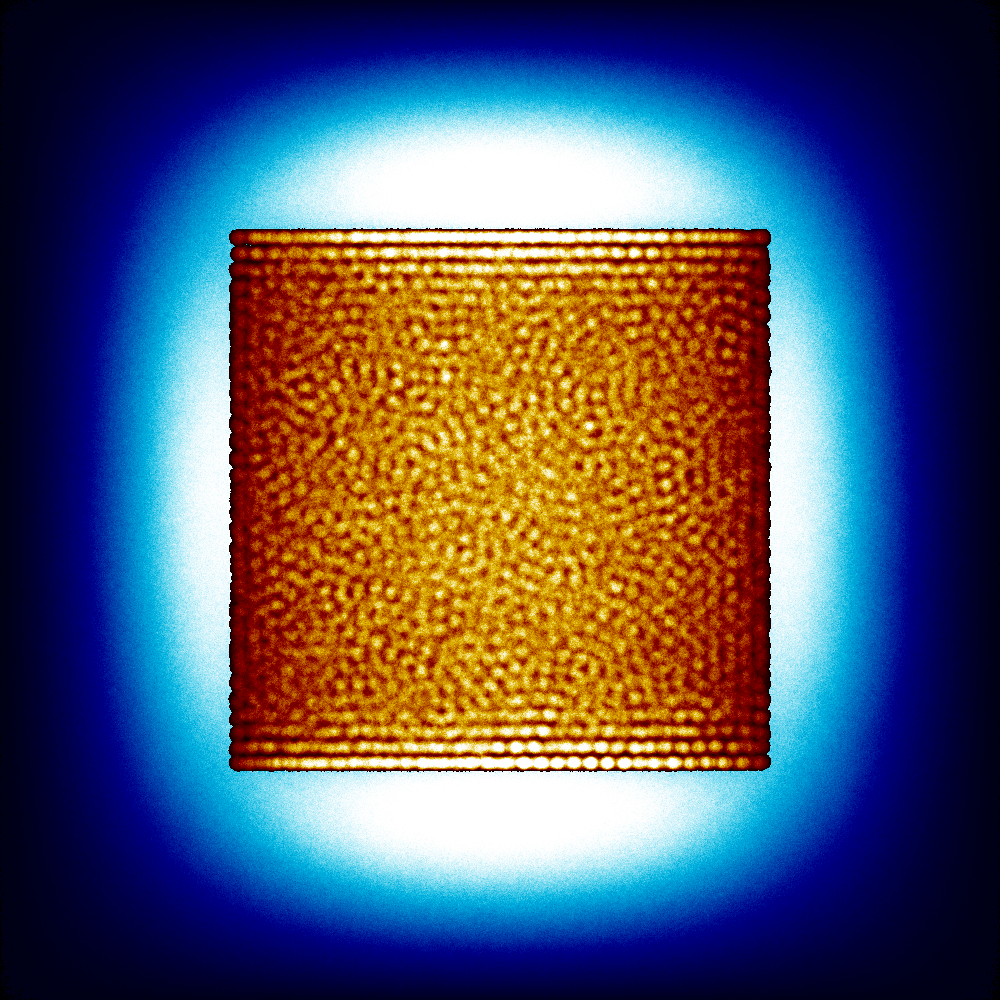
\includegraphics[width=0.95\linewidth]{figures/control/control-vm}
  \caption{Axial Mesh}
  \label{fig:controld}
\end{subfigure}
%
\begin{subfigure}{\textwidth}
\centering
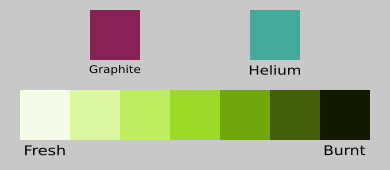
\includegraphics[width=0.6\linewidth]{figures/geom-legend}
\caption{Legend for \ref{fig:controla} and \ref{fig:controlc}}
\label{fig:geom-legend1}
\end{subfigure}

\caption{Geometry Cross Sections (left) and Thermal Flux(cold color map) and Fission Rate (hot color map) Meshes (right) for the Control Model of Sangamon20}
\label{fig:controlmain}
\end{figure}

Figure \ref{fig:controlb} shows bands of concentric rings around the outer edges of the active core.  These bands suggest that there is pebble alignment at the edge of the core, and that the outermost areas of the core are regions of high fission activity relative to the center.  Certainly the pebbles are physically forming rings at the outer edges, and their placement becomes less structured toward the center.  However, the high intensities seen in this outer region in the mesh figures are unindicative of a total flux profile showing the same.  Recall that Serpent integrates over the z direction to produce a 2D plot of the xy plane.  For a cylinder, the distance in z each point integrates over is the same - the height of the reactor.  However, points at the outermost regions are integrating in a volume composed more of pebbles - and therefore fissile material - than the center, where more space filled with coolant.  The outer regions are more regularly packed with pebbles - and therefore have less coolant than the center - because the dispersal routine (and the grow and shake algorithm) naturally cause the pebbles to line up along the reactor boundary.  Lattice arrangements wouldn't have this feature because these methods ignore core boundaries.

In Figure \ref{fig:controld} we can see a similar banding effect on the top and bottom edge of the core region, but not on the sides.  No hot-spots on the edges because Figure \ref{fig:controld} is in the xz plane, and integrates over y.  However, for a cylinder, the distance integrated over is not the same at all points.  At the centerline, the distance is simply the diameter.  However, as you move towards the edge, the distance integrated over approaches zero.  So, while these plots can help provide some insight into the core, one must be very careful to keep this uneven integration area in mind when interpreting them.

Figures \ref{fig:hom-det-xy} and \ref{fig:hom-det-z} provide the fast and thermal flux profiles in the control model of Sangamon20, which uses homogenized pebbles, at the axial and radial (x-direction) centerlines, respectively.  Bin size in the detectors was selected based on reactor geometry and the average diffusion length of neutrons in graphite \cite{hereward_measurement_1947}.

\begin{figure}[H]
\centering

\begin{subfigure}{0.9\textwidth}
  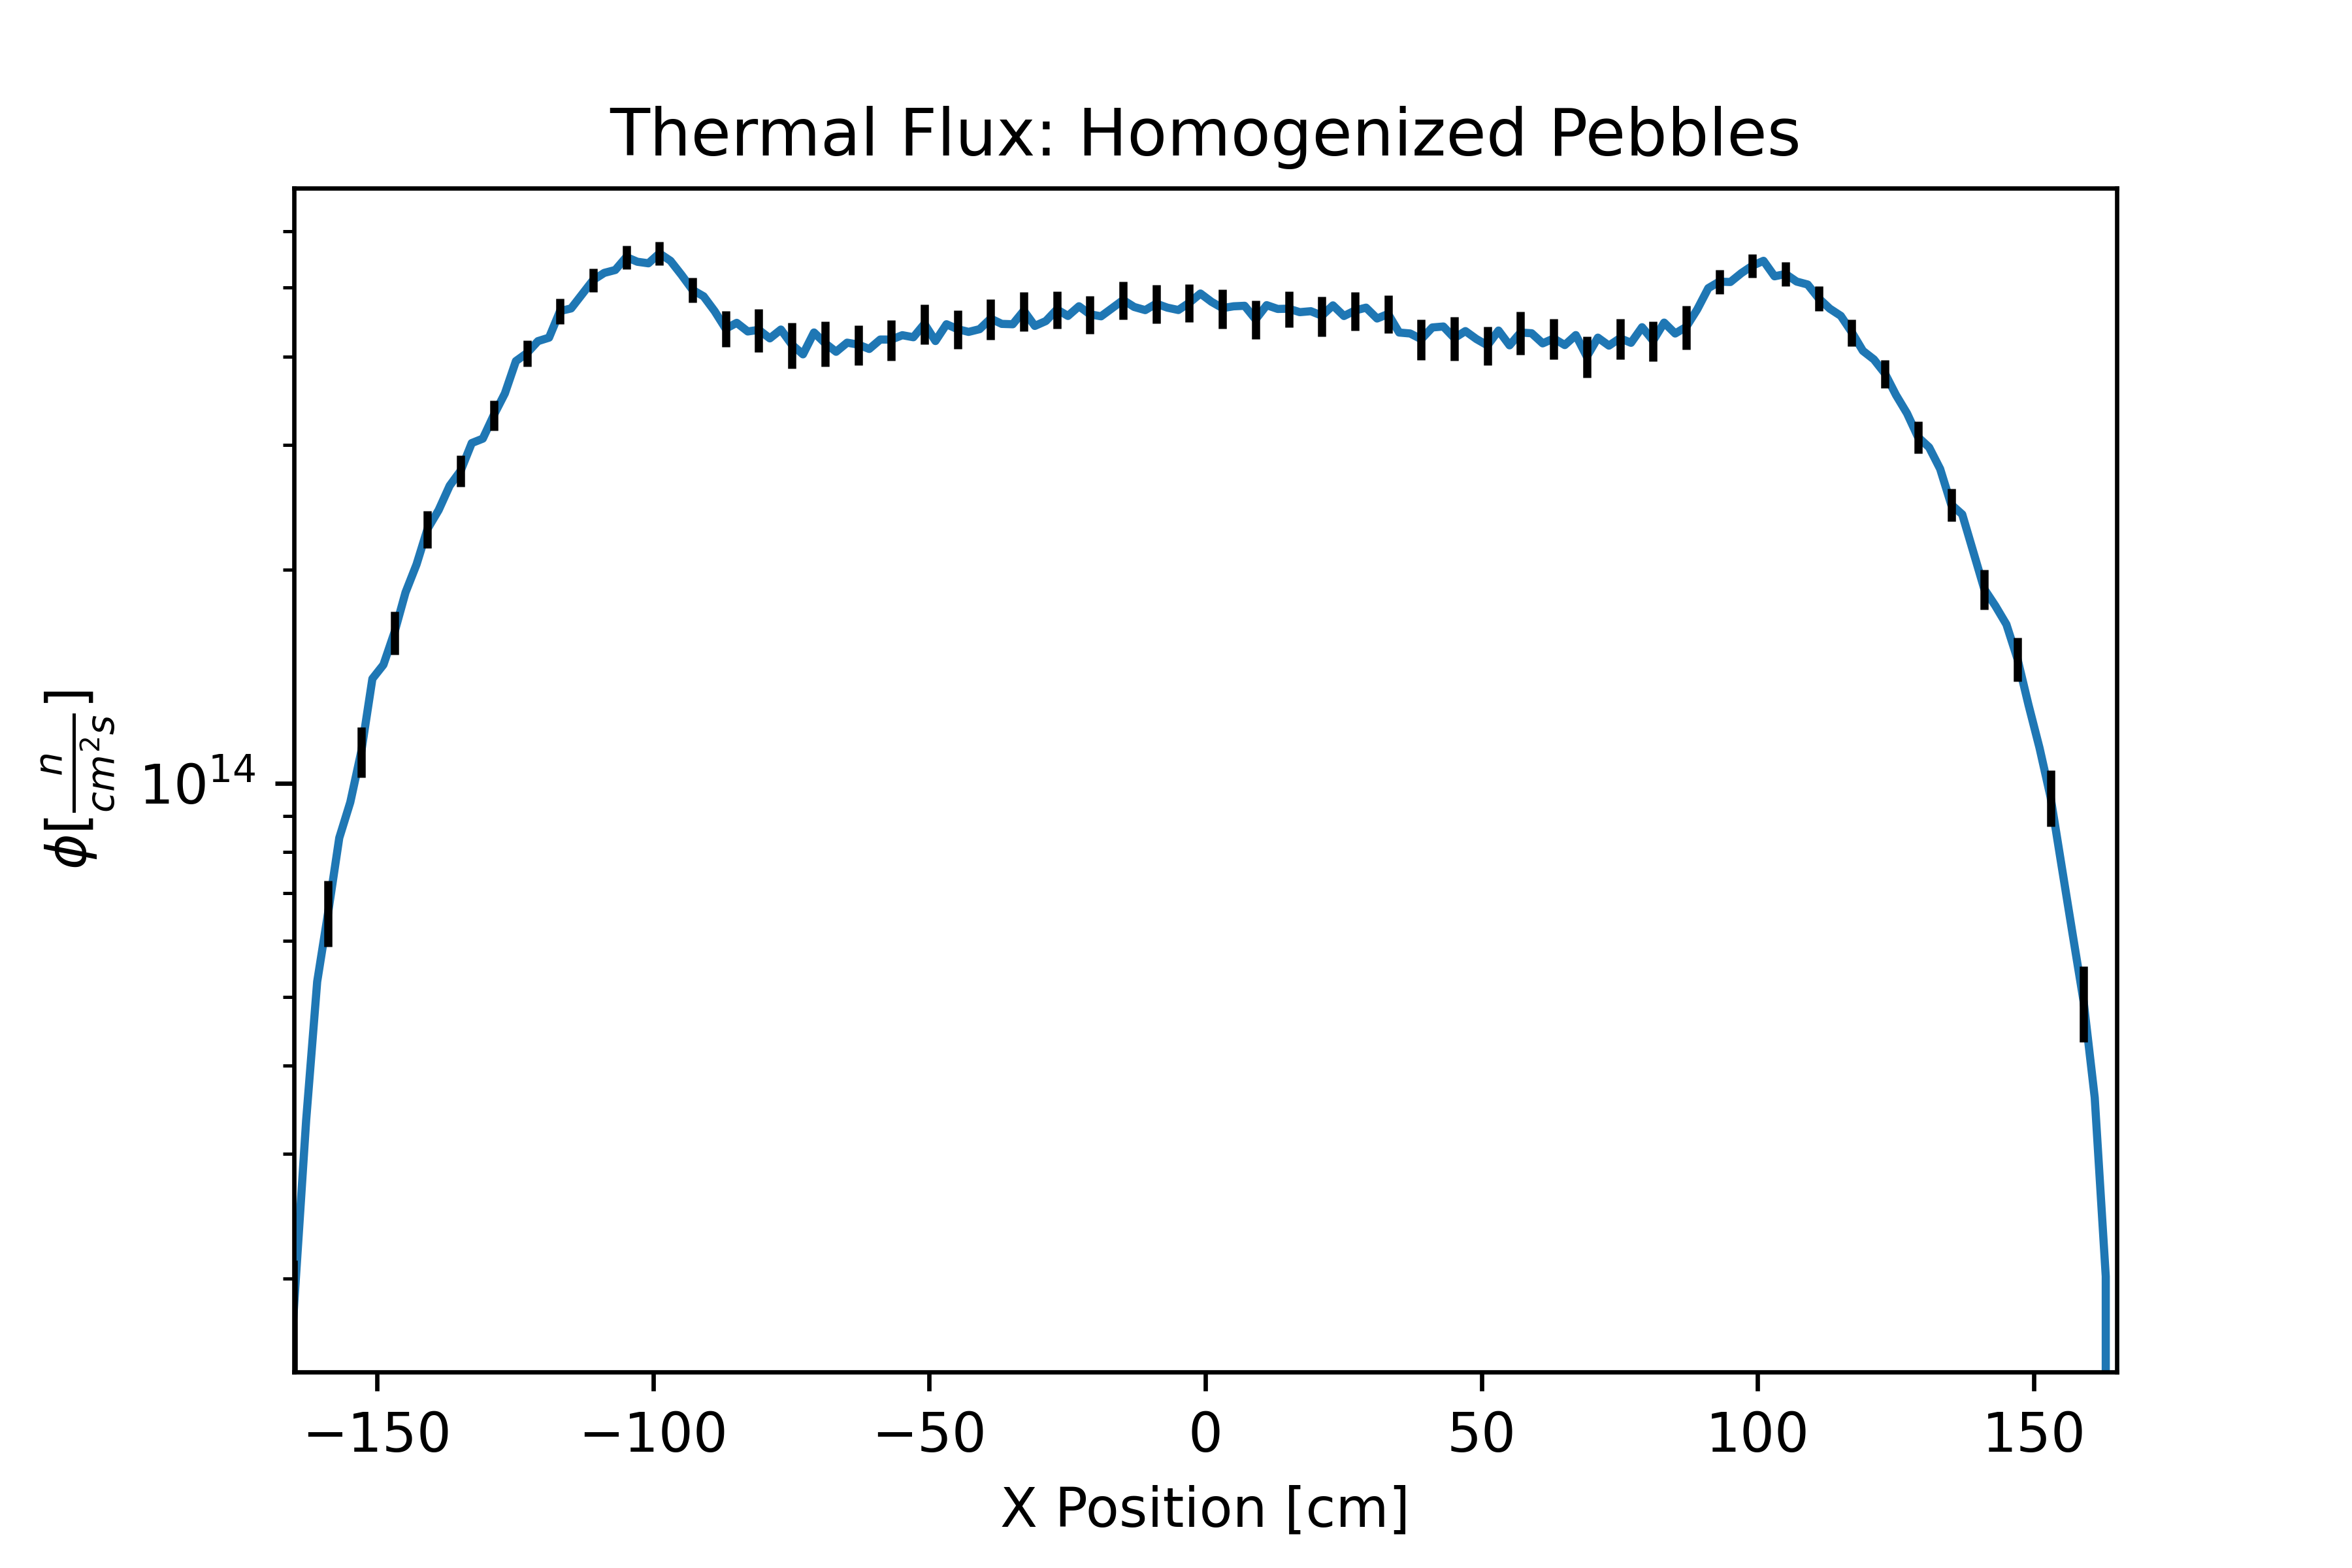
\includegraphics[width=0.95\linewidth]{figures/therm_flux_homog.png}
  \caption{Thermal Flux}
  \label{fig:hom-det-xy-therm}
\end{subfigure}%

\caption{Radial Thermal and Fast Flux Profiles}
\end{figure}

\begin{figure}[H]\ContinuedFloat
\centering

\begin{subfigure}{0.9\textwidth}
  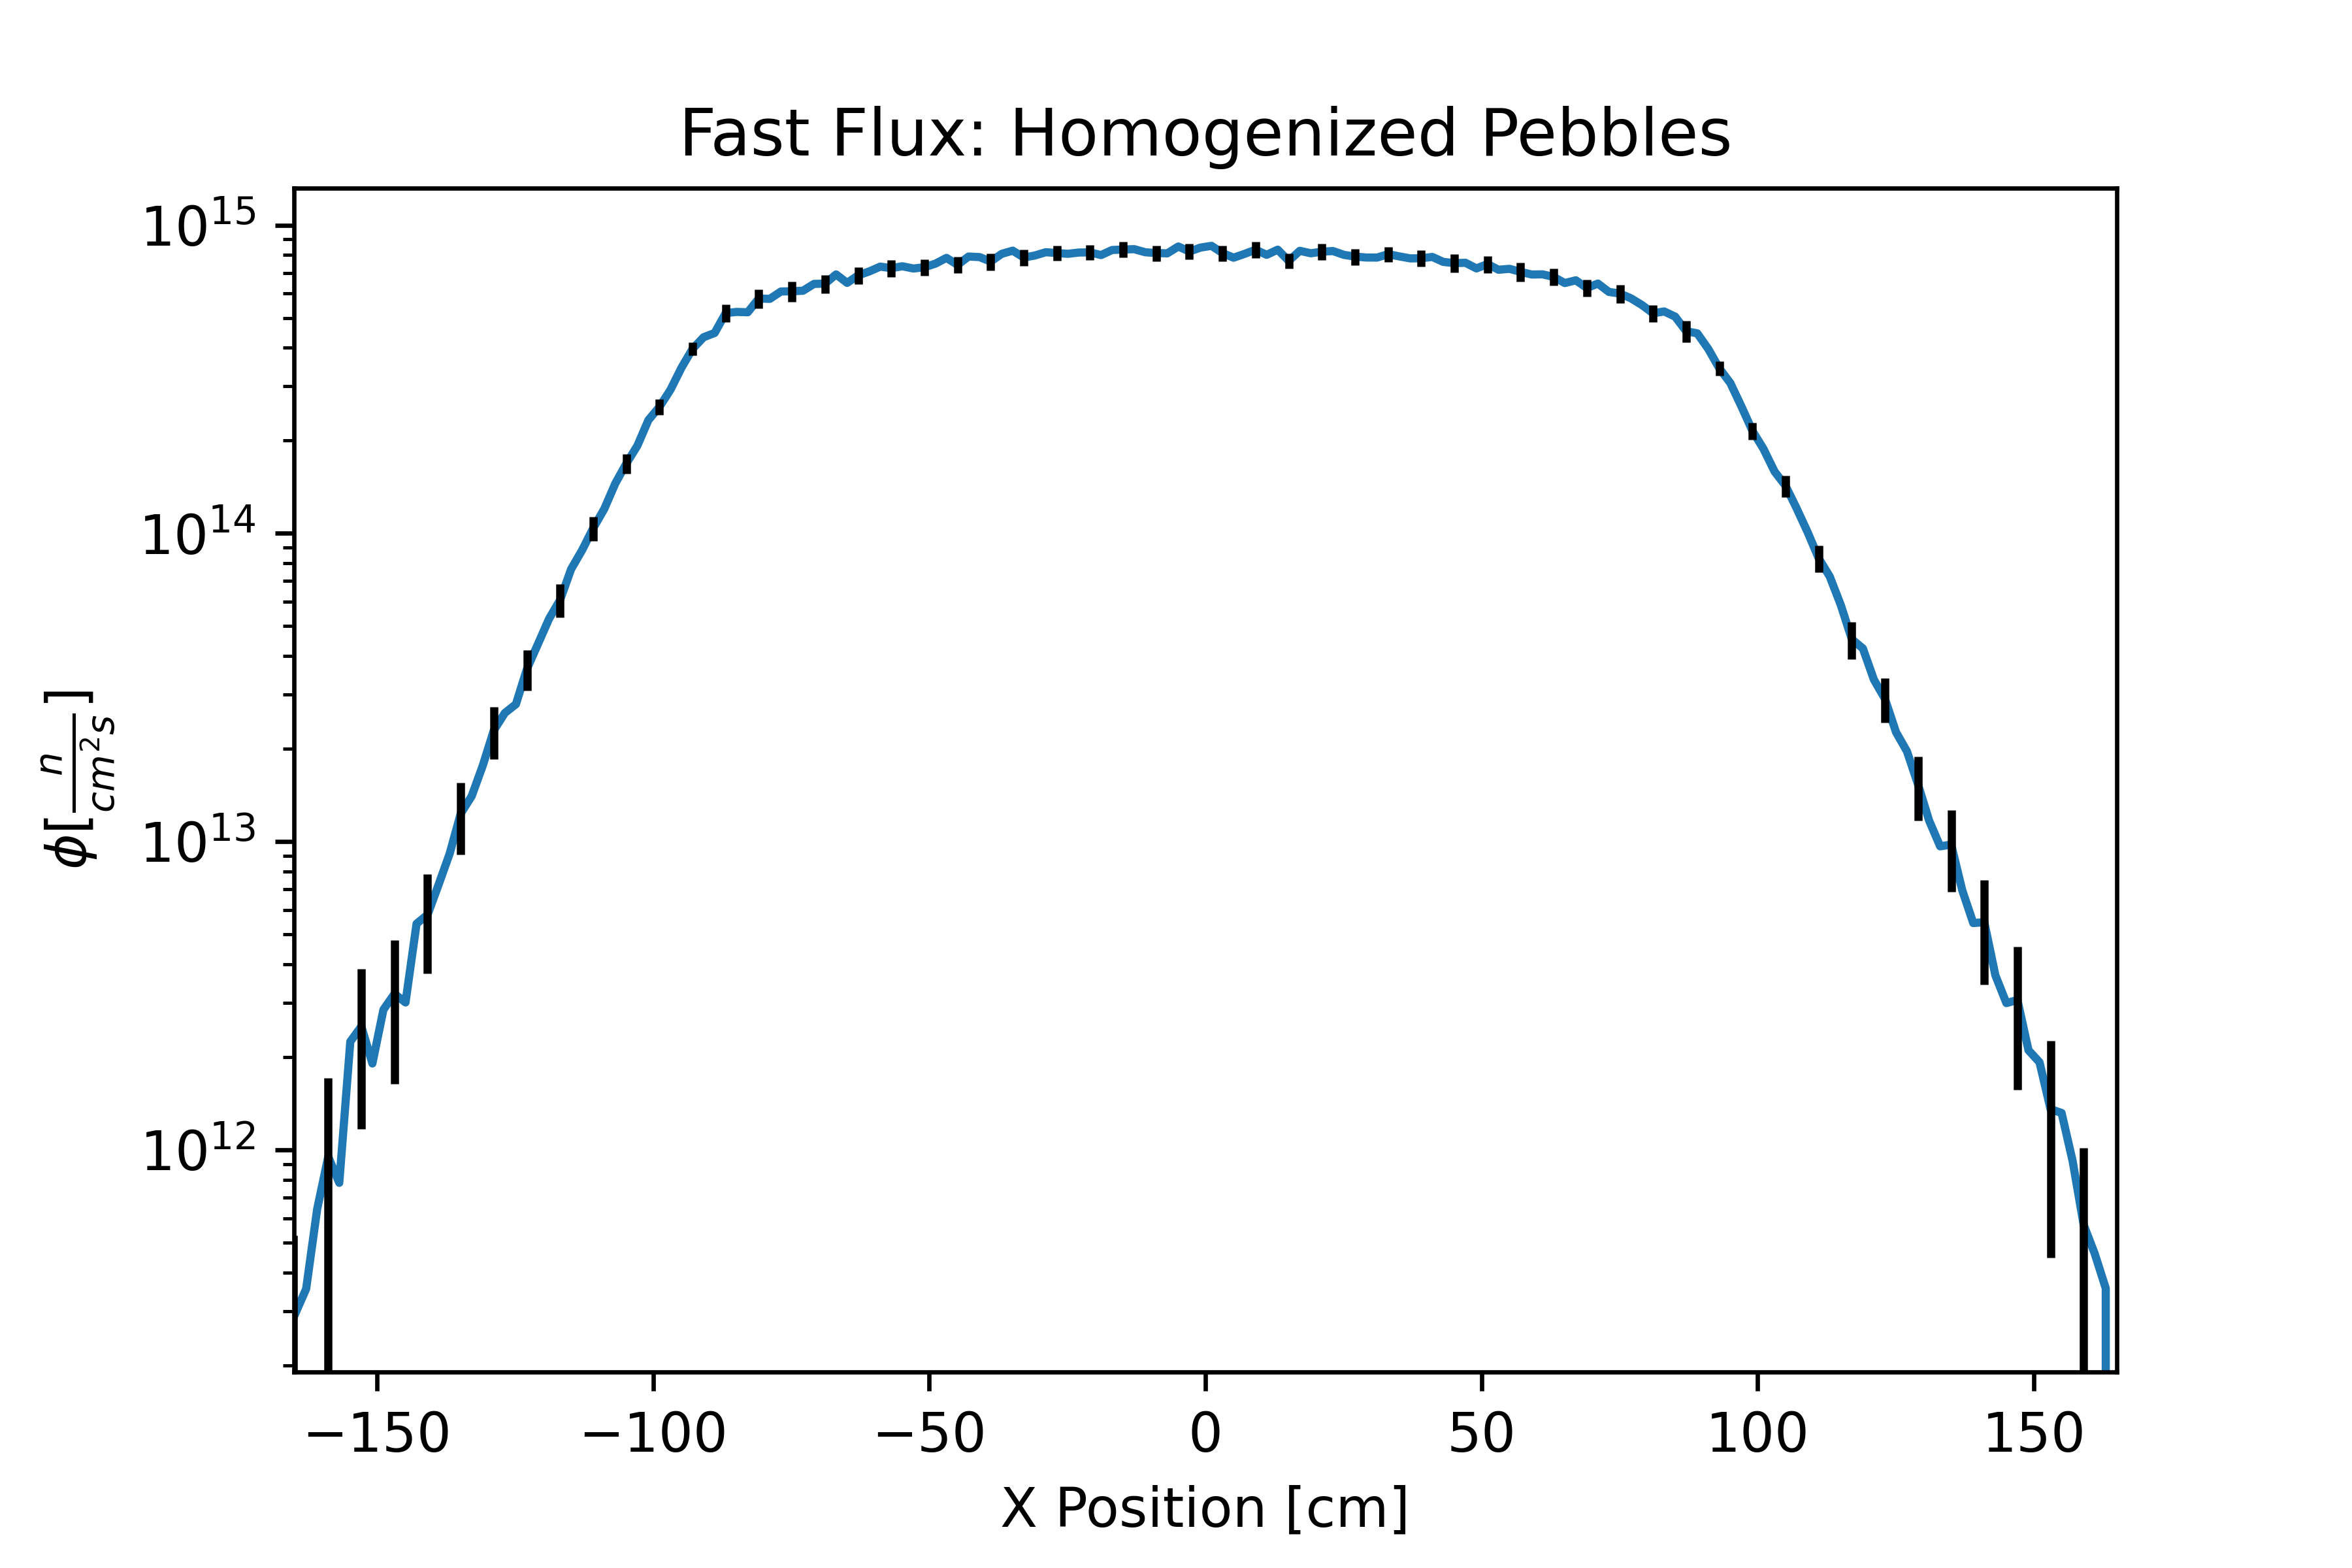
\includegraphics[width=0.95\linewidth]{figures/fast_flux_homog.png}
  \caption{Fast Flux}
  \label{fig:hom-det-xy-fast}
\end{subfigure}

%
\caption{Radial Thermal and Fast Flux Profiles (cont.)}
\label{fig:hom-det-xy}
\end{figure}
\begin{figure}[h!]
\centering

\begin{subfigure}{0.6\textwidth}
  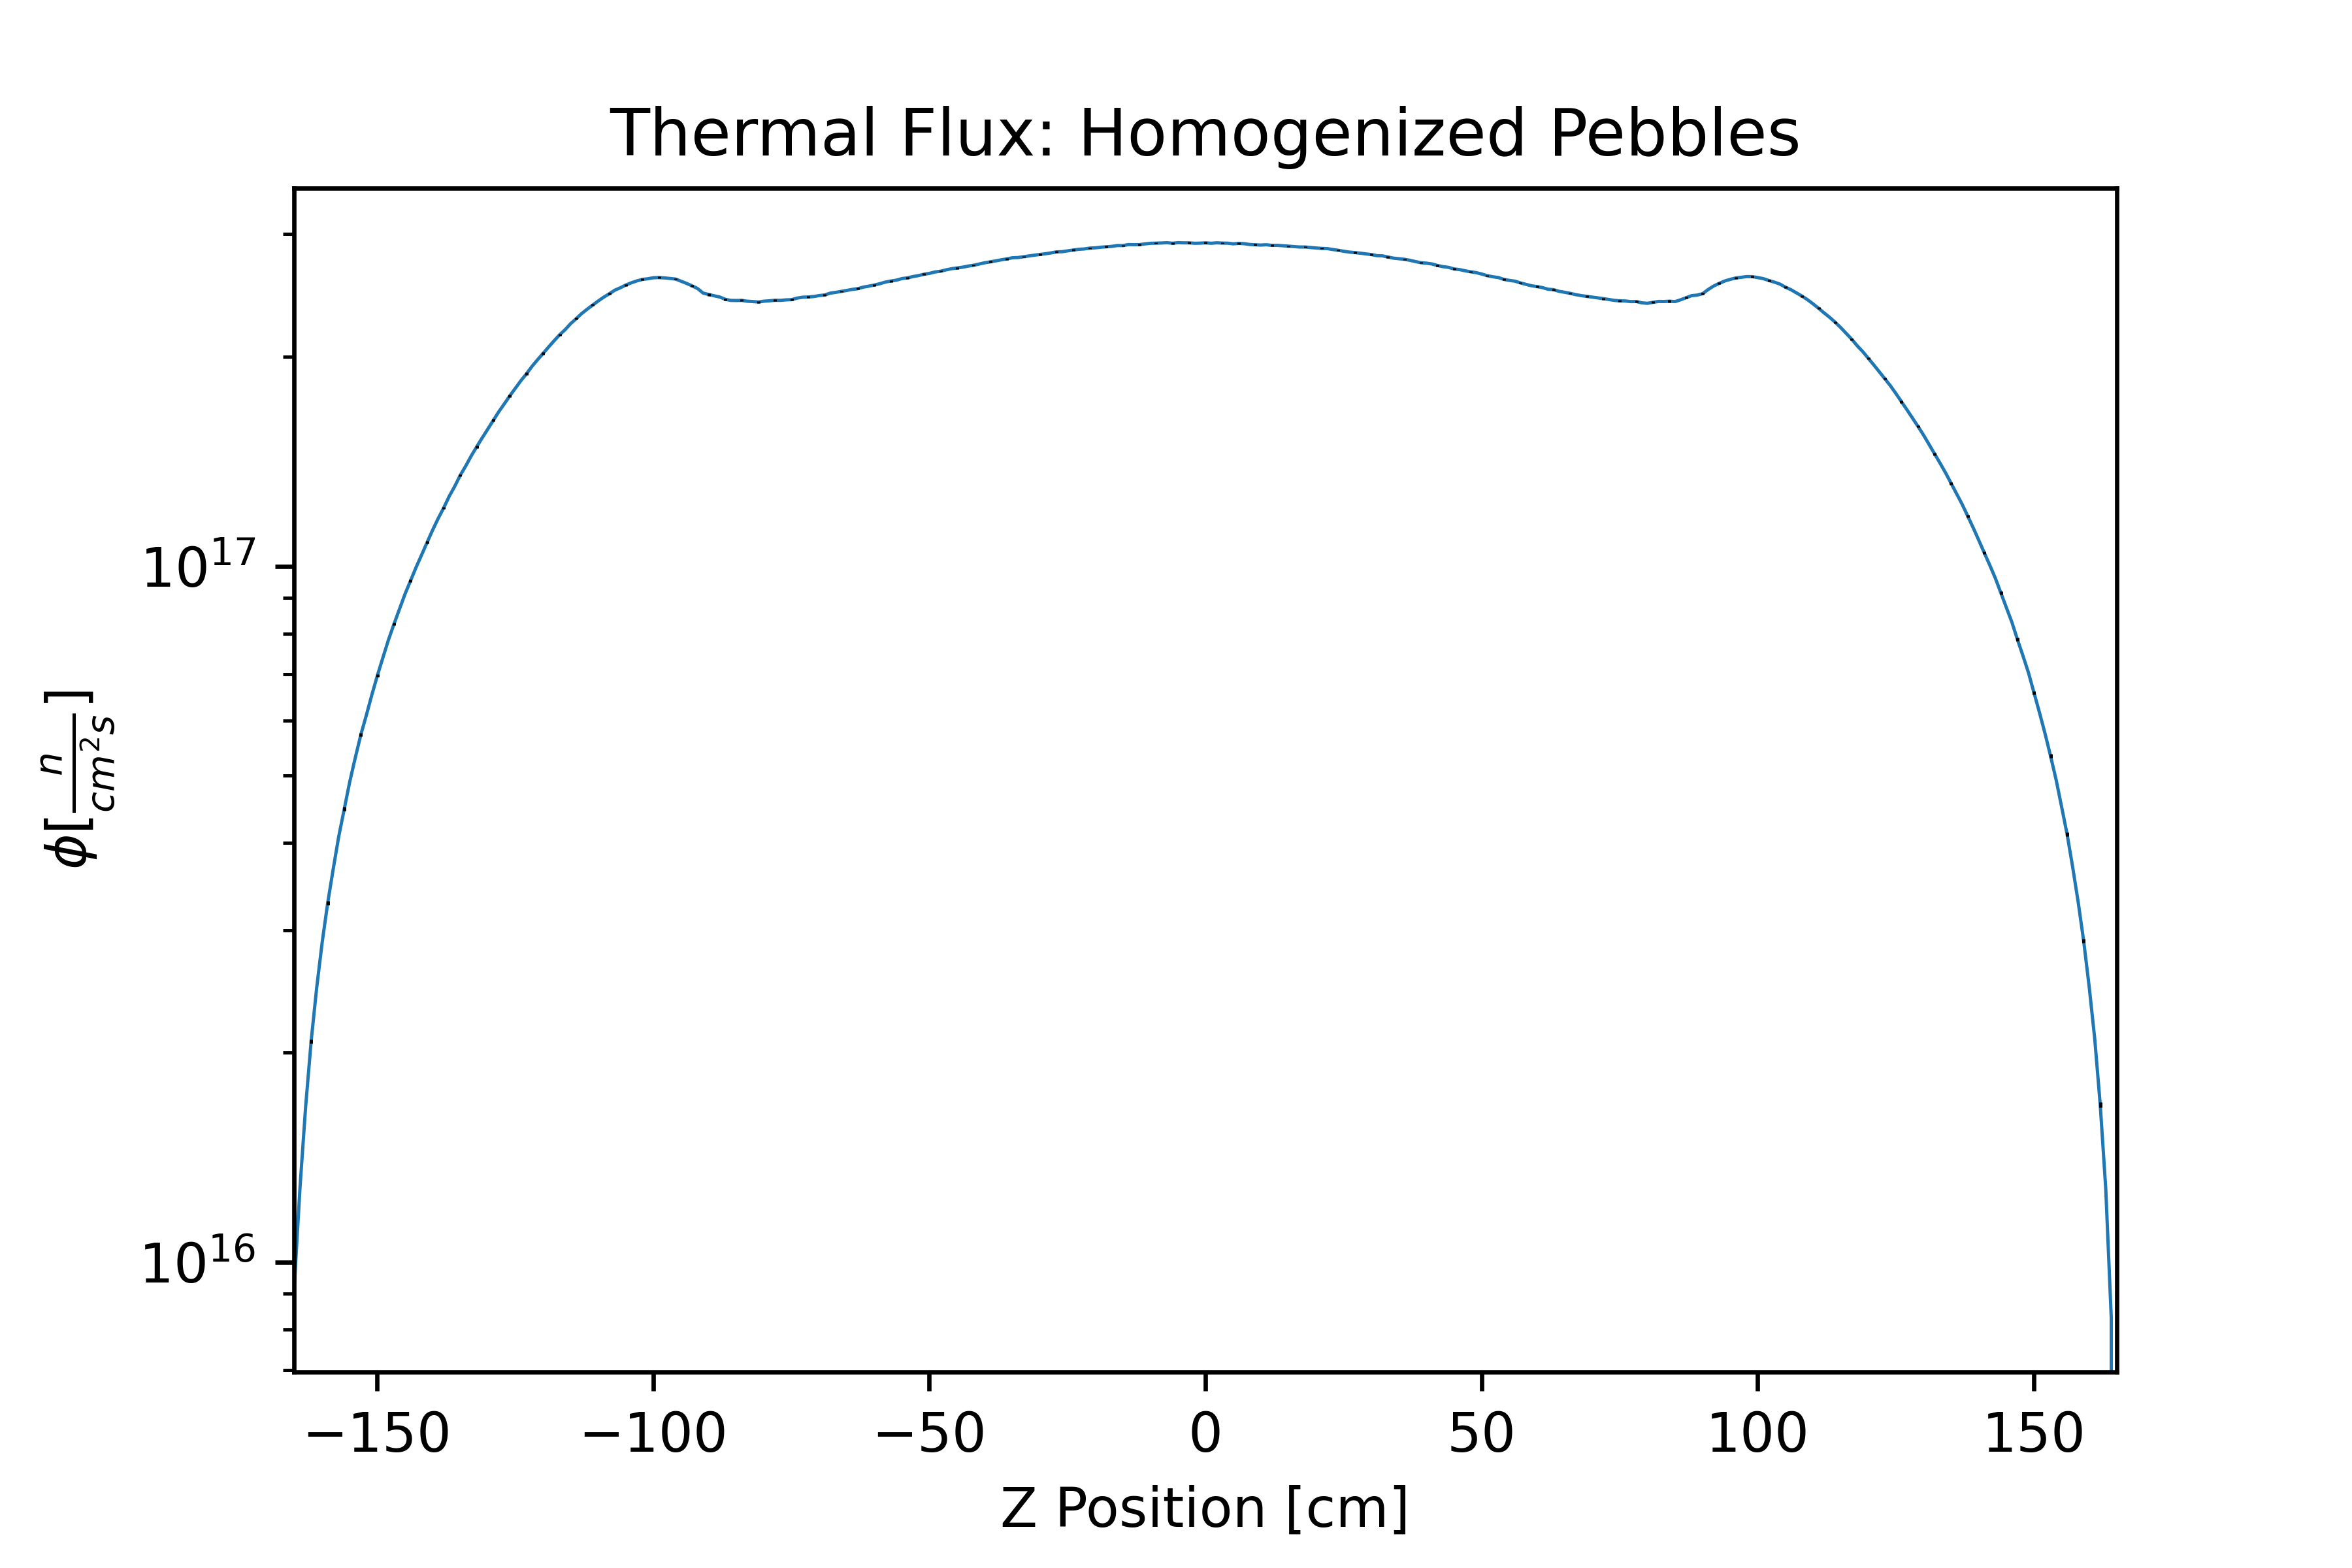
\includegraphics[width=0.95\linewidth]{figures/therm_flux_homog_z.png}
  \caption{Thermal Flux}
  \label{fig:hom-det-z-therm}
\end{subfigure}%
%
\begin{subfigure}{0.6\textwidth}
  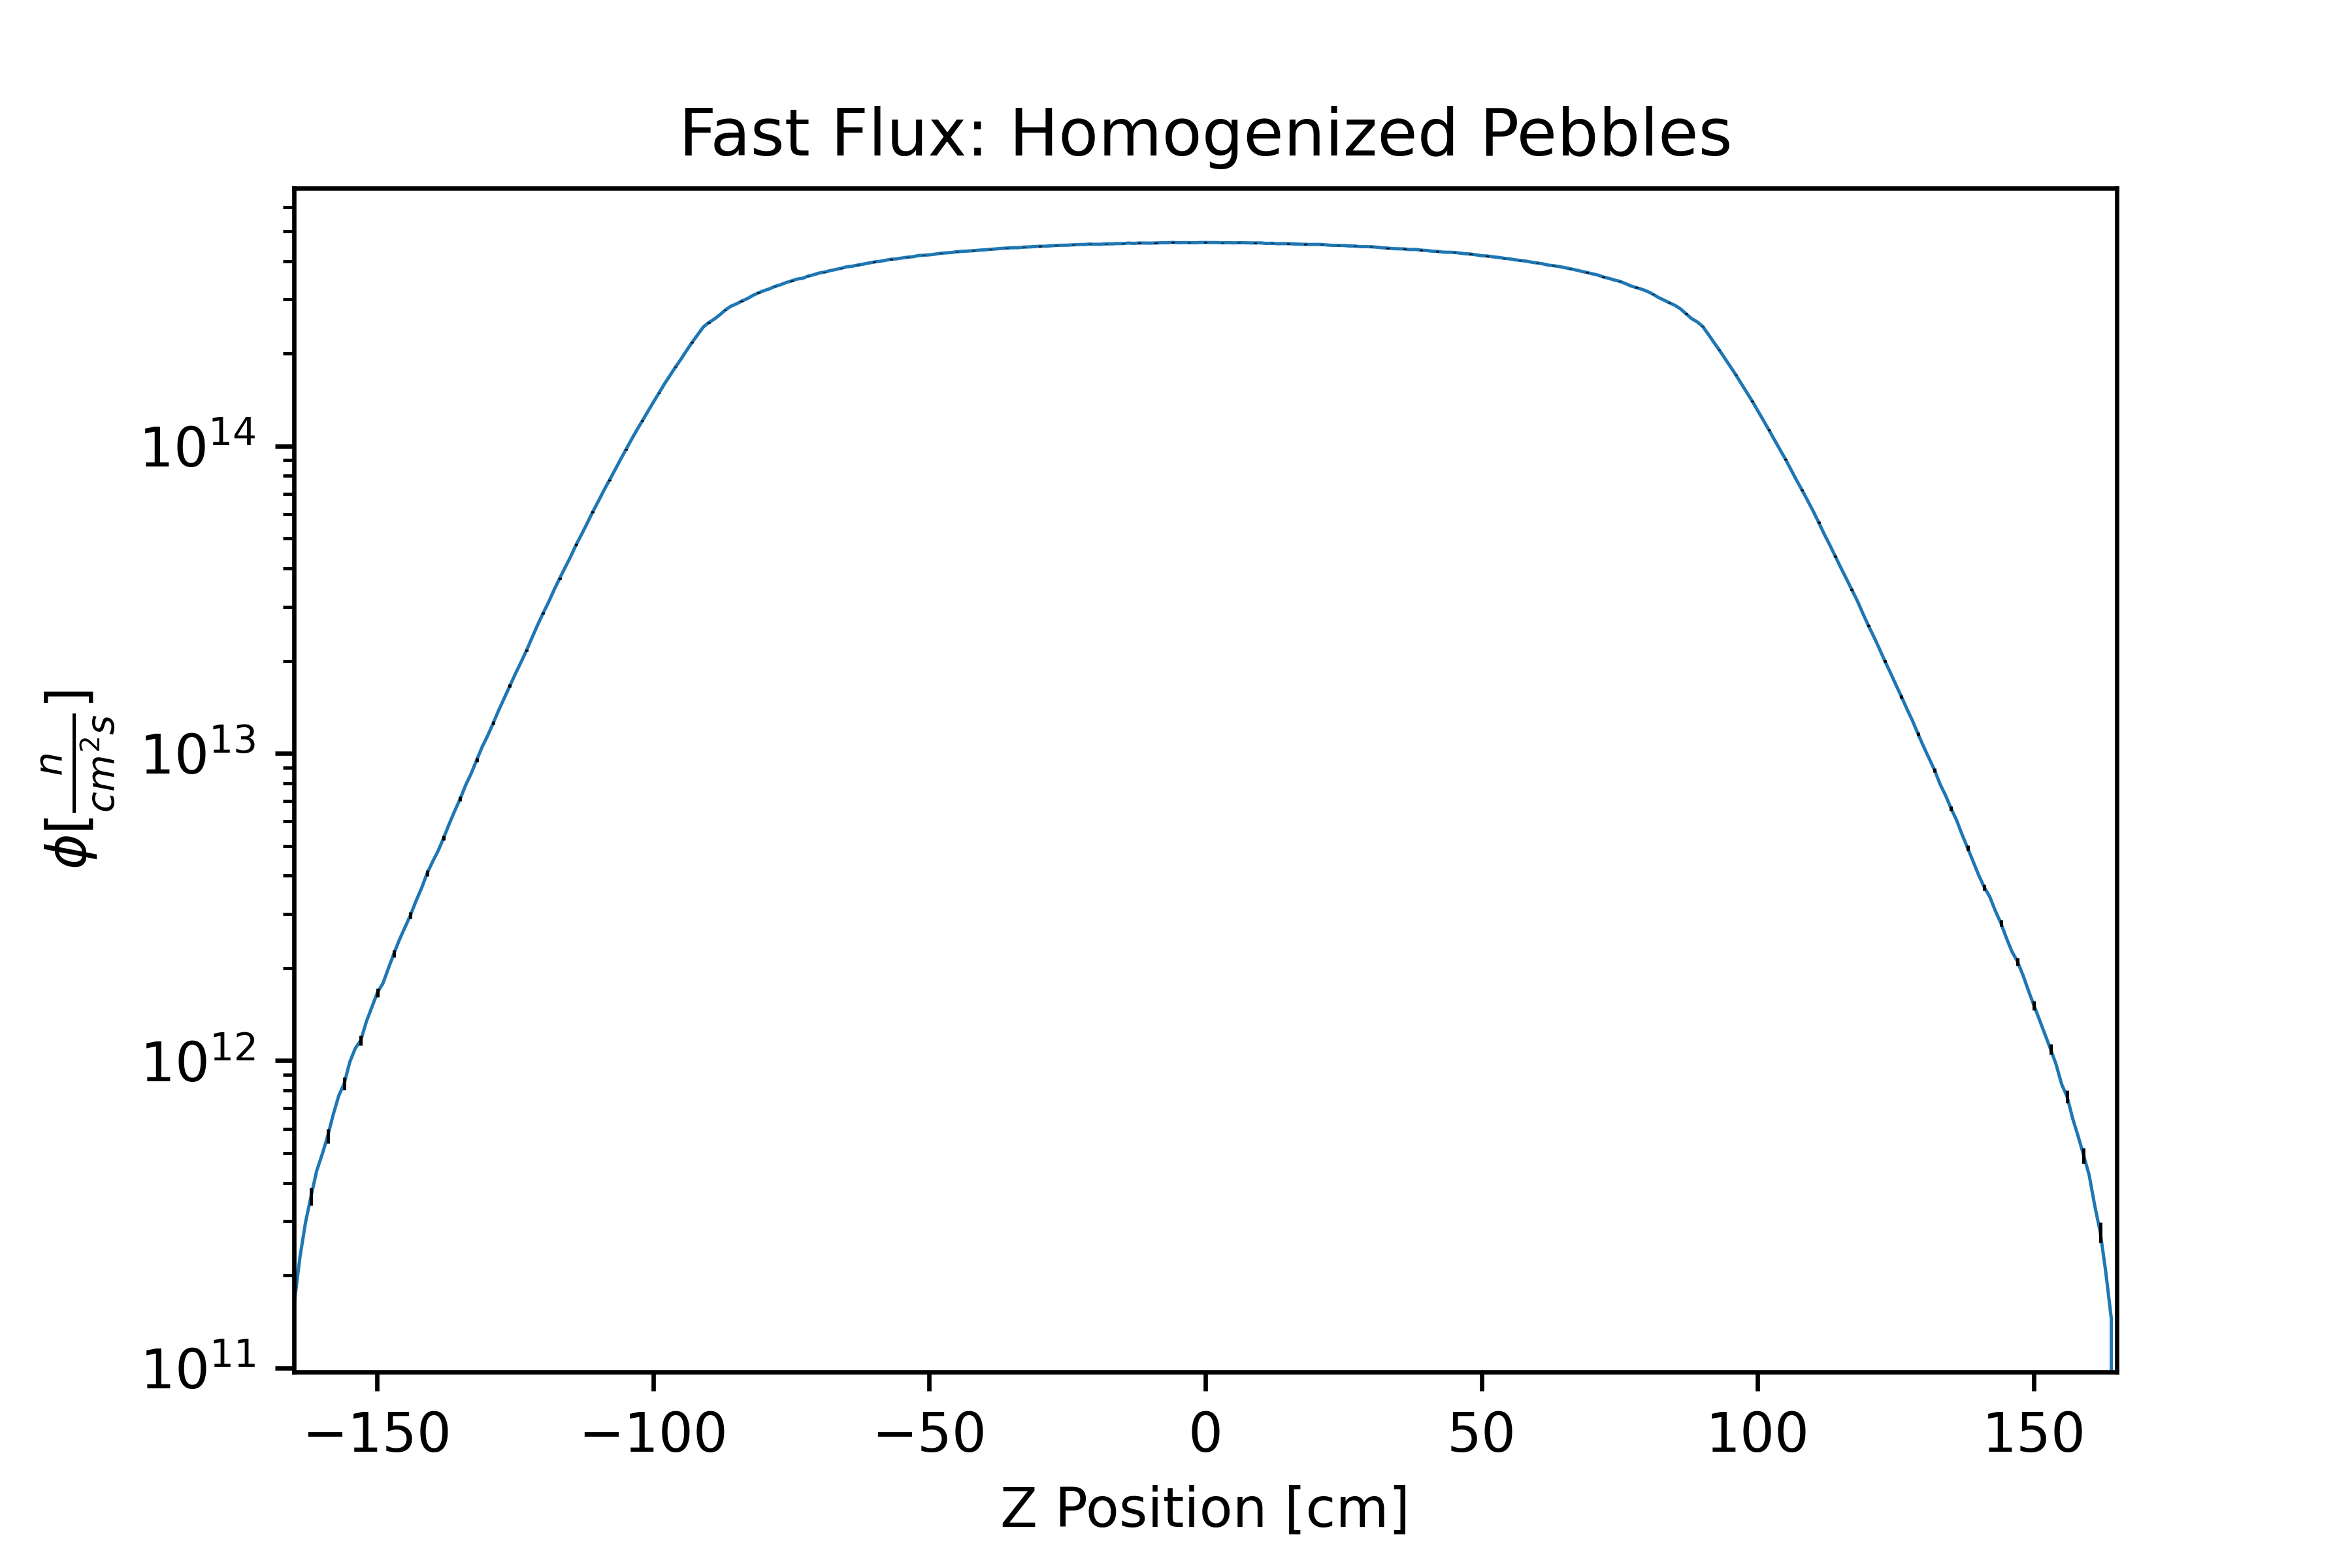
\includegraphics[width=0.95\linewidth]{figures/fast_flux_homog_z.png}
  \caption{Fast Flux}
  \label{fig:hom-det-z-fast}
\end{subfigure}

%
\caption{Axial Thermal and Fast Flux Profiles}
\label{fig:hom-det-z}
\end{figure}

For the radial flux, a detector in the xy plane was used, which had finite bin sizes in x and y, and spanned the whole height of the reactor in the z direction.  For the axial fluxes, the bins were finite in z and spanned the entire diameter of the core.  Normally, these two figures would be subject to the same unequal bin sizing that affected Figure \ref{fig:controlmain}.  To counteract this, the axial fluxes (Figure \ref{fig:hom-det-z}) are multiplied by the ratio of the radial detector bin volume to the axial detector bin volume, as follows:

\begin{align}
\phi_{axial, adjusted} &= \phi_{axial, unadjusted}\frac{V_{radial}}{V_{axial}}
\intertext{where}
\phi_{axial, adjusted}&= \mbox{ detector bin-size adjusted flux $\left[\frac{\#}{cm^2s}\right]$}\nonumber\\
\phi_{axial,unadjusted}&= \mbox{ unadjusted axial flux $\left[\frac{\#}{s}\right]$}\nonumber\\
V_{radial}&=\mbox{ radial detector bin volume $[cm^3]$}\nonumber\\
V_{axial}&=\mbox{ axial detector bin volume $[cm^3]$}\nonumber
\end{align}

Both axially and radially, the thermal flux sees a 'bump', which peaks approximately 10 $\left[cm\right]$into the reflector, at 100 $\left[cm\right]$.  These are the highest peaks in the thermal flux, with the second highest thermal flux being at the center line.  For the fast flux profile we see a flattened peak in the  active core (-90.0 $\left[cm\right]$ to 90 $\left[cm\right]$).  Fast flux rapidly decreases in the reflector as fast neutrons down scatter in the graphite.  Both Figures \ref{fig:hom-det-xy} and \ref{fig:hom-det-z} show that the flux peaks are at the core centerline, as expected.

In addition to centerline fast and thermal flux profiles, Figures \ref{fig:hom-plane-fast} and \ref{fig:hom-plane-therm} provide a heatmap of the fast and thermal flux profiles in the xy plane.

\begin{figure}[H]
\centering

  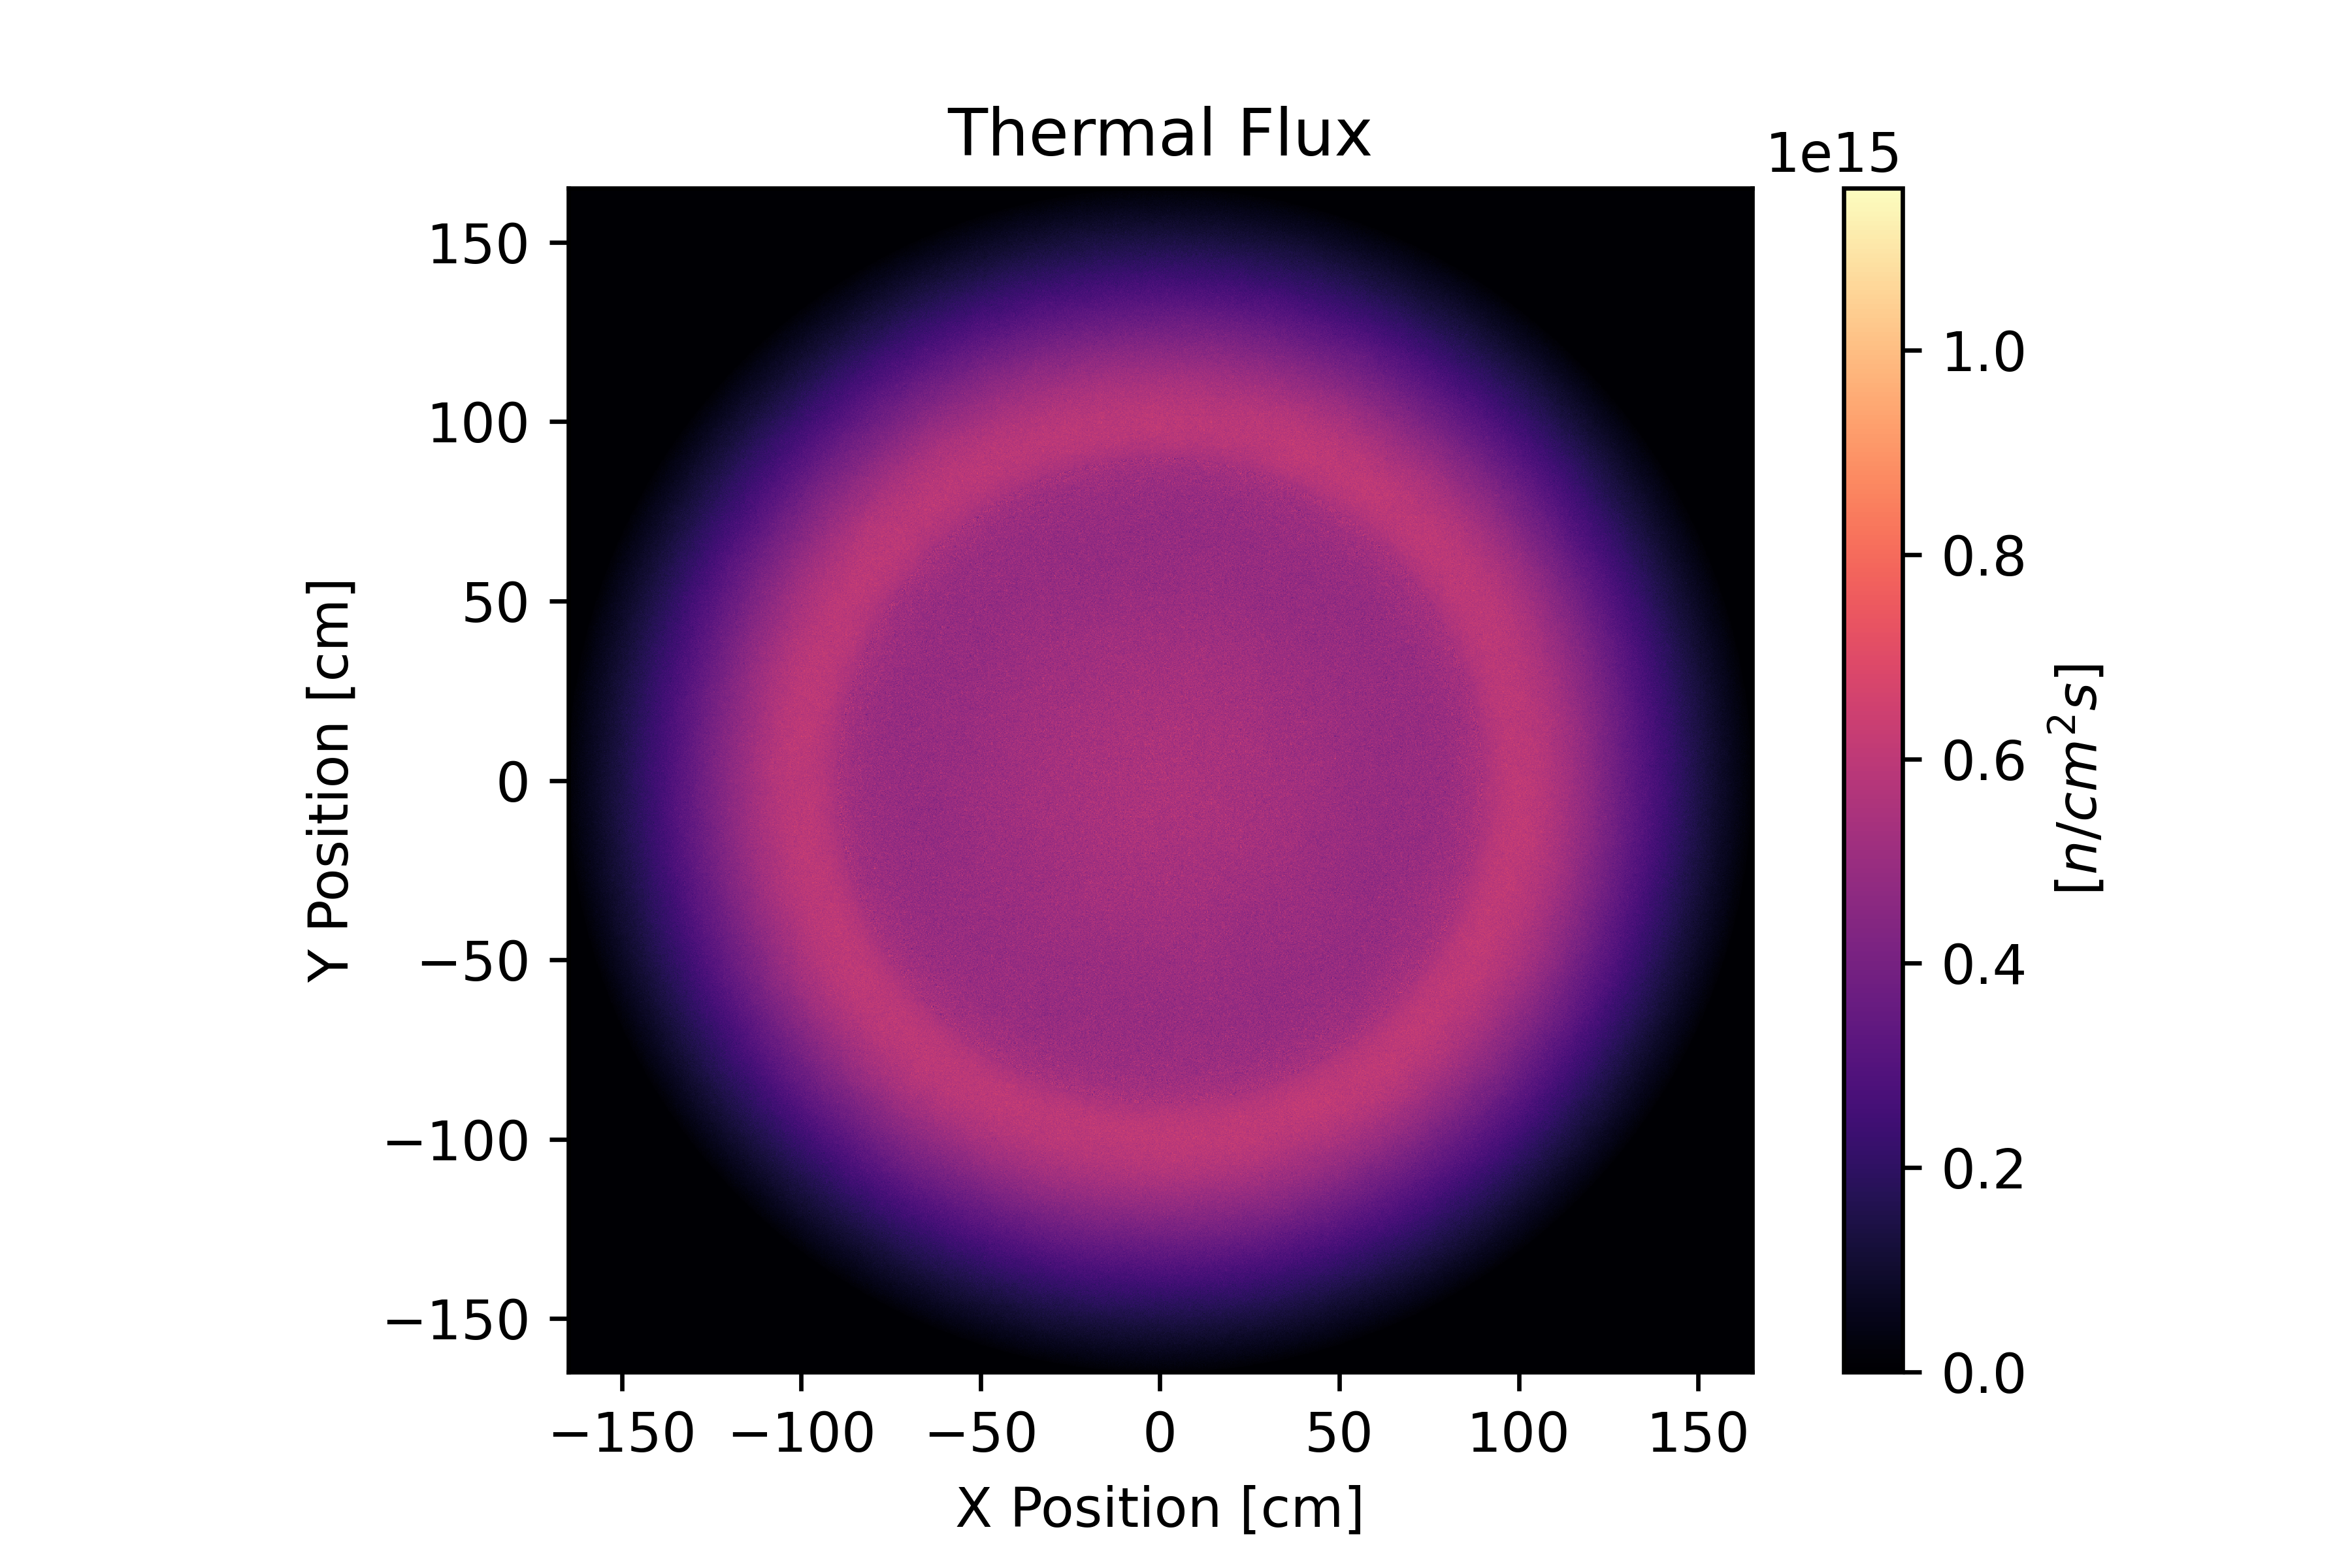
\includegraphics[width=1.0\linewidth]{figures/therm_xy_plane_homog_er.png}
  \caption{Thermal Flux in xy Plane in Sangamon20: Homogenized Pebbles.  The dotted line annotation marks the boundary between the active core and the graphite reflector.}
  \label{fig:hom-plane-therm}

\end{figure}


\begin{figure}[H]
\centering

 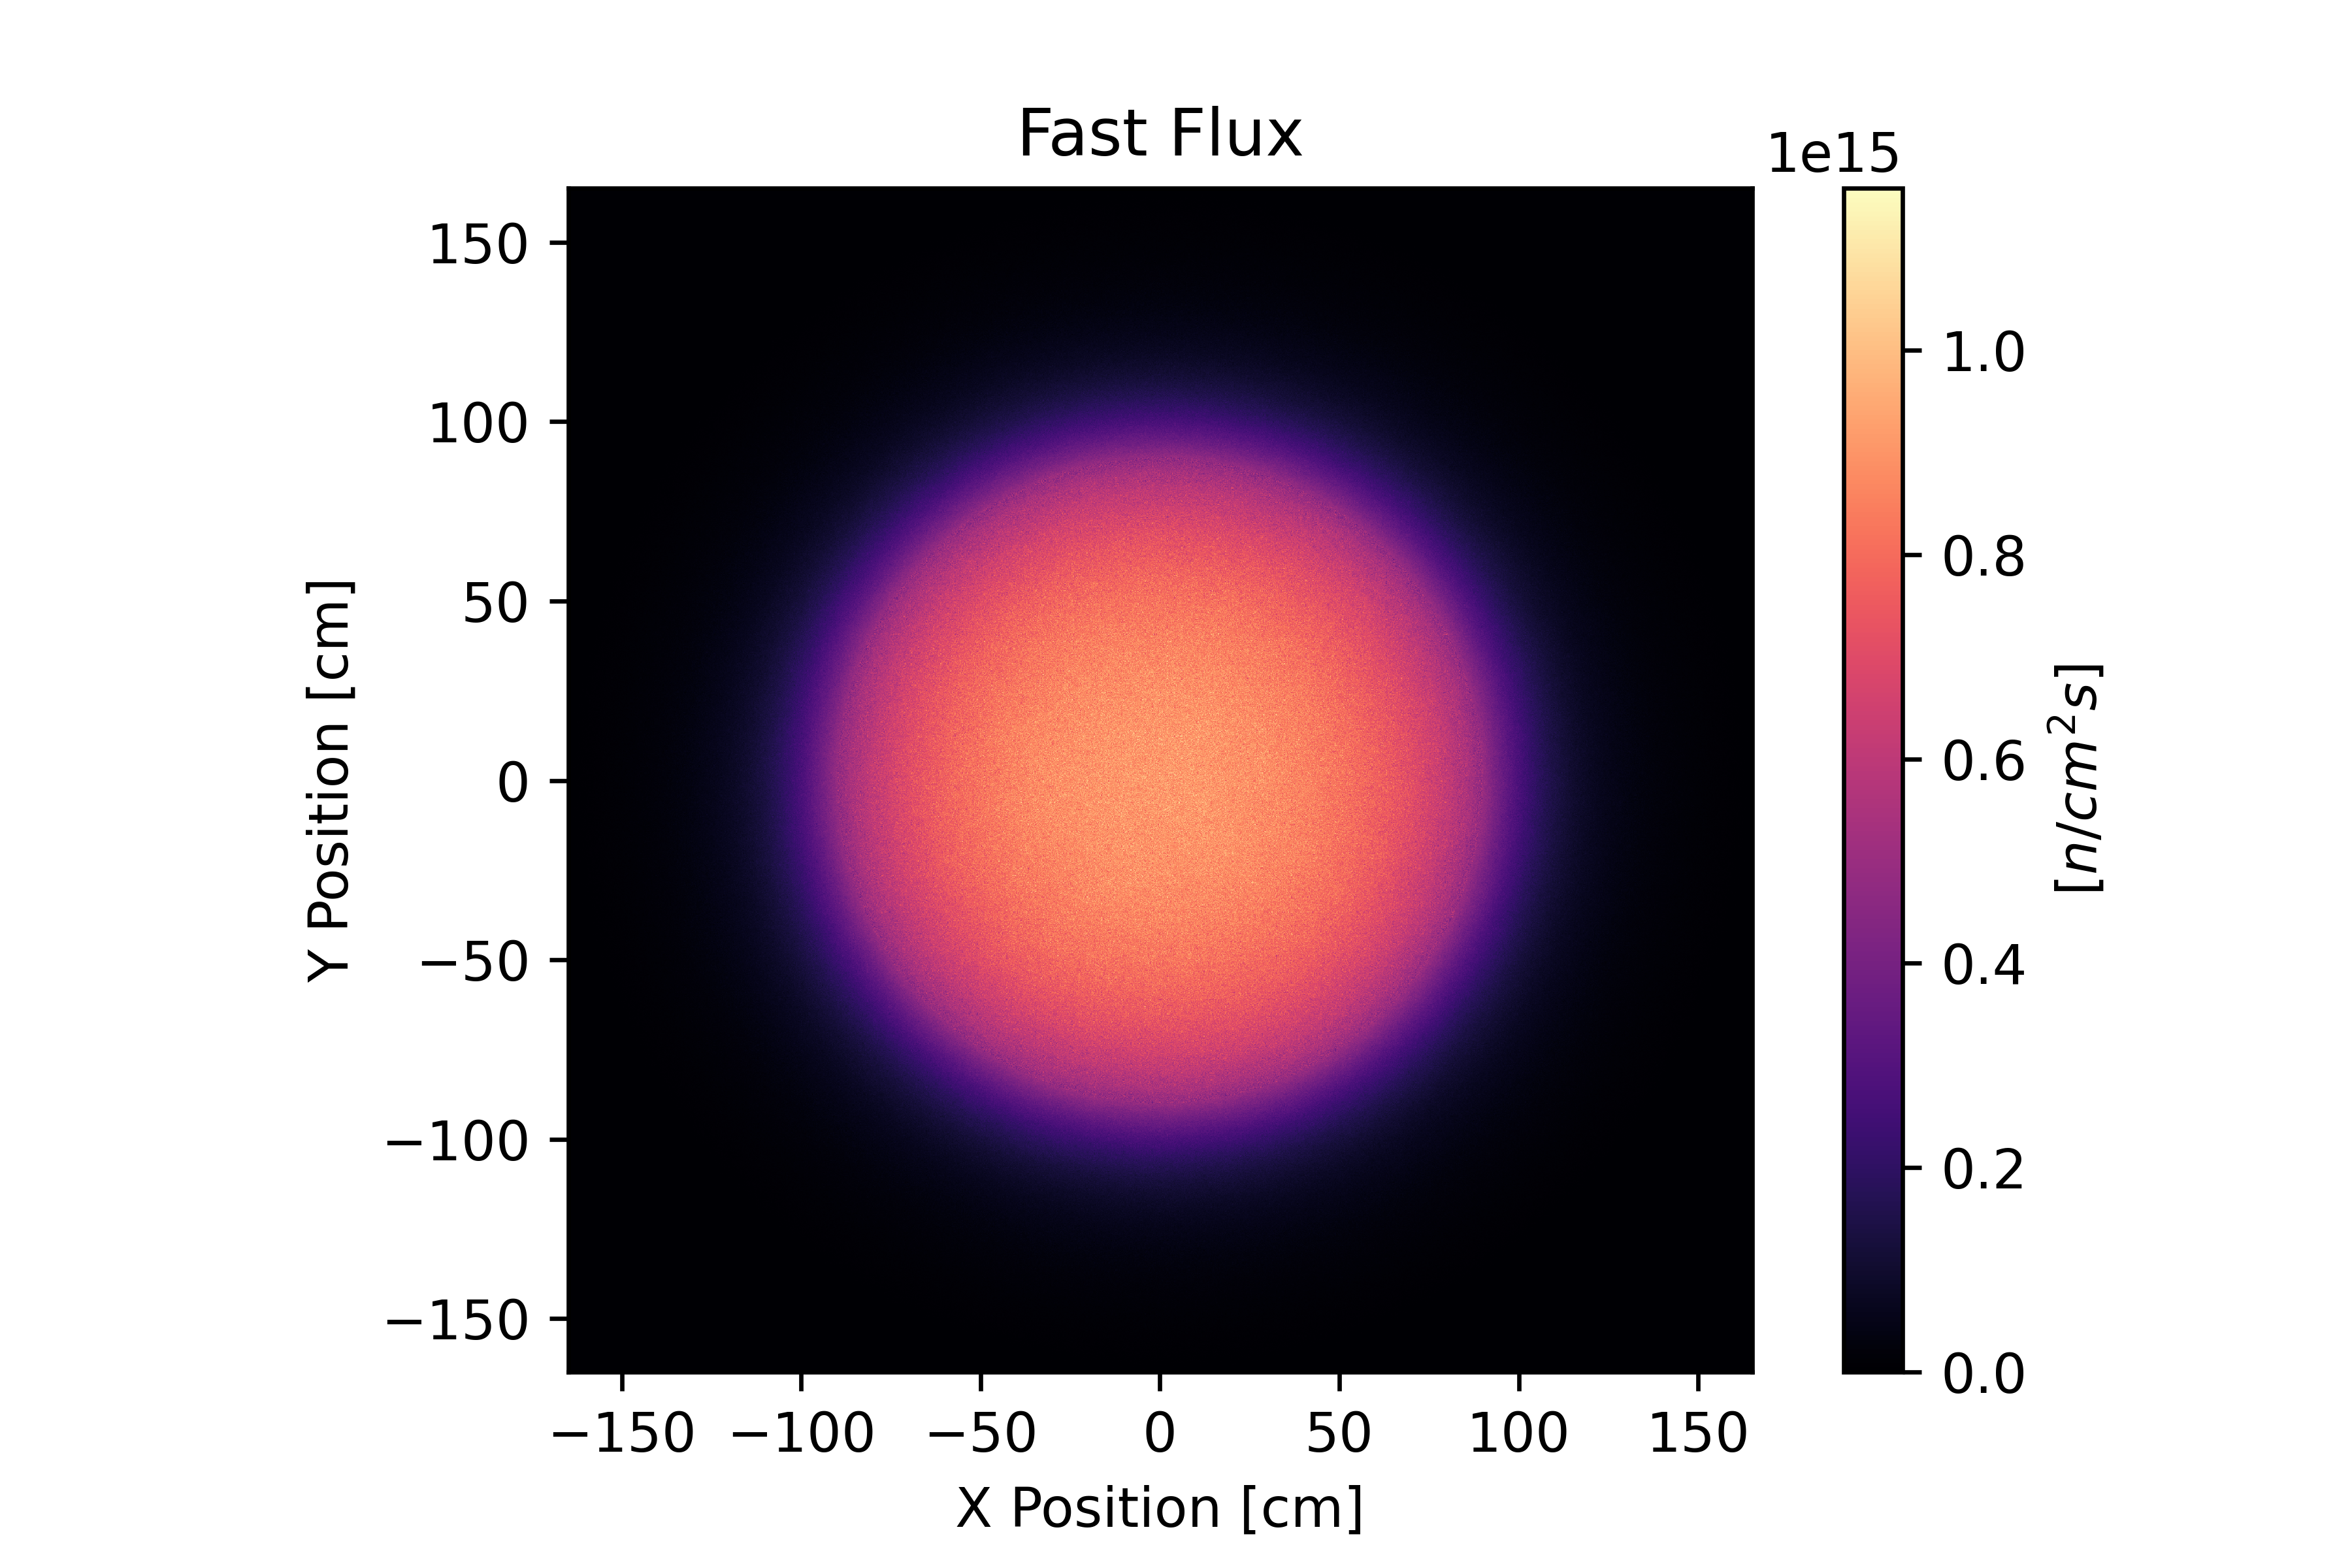
\includegraphics[width=1.0\linewidth]{figures/fast_xy_plane_homog_er.png}
 \caption{Fast Flux in xy Plane in Sangamon20: Homogenized Pebbles.  The dotted line annotation marks the boundary between the active core and the graphite reflector.}
 \label{fig:hom-plane-fast}

\end{figure}

A slight banding pattern on the active core's edge exists --- primarily in the fast, rather than thermal, flux --- but with less intensity than the fission rate banding.  In the thermal flux, we see that the peak in \ref{fig:hom-det-xy} continues in a circular pattern surrounding the active core, approximately 10 cm into the graphite reflector.  The steep drop-off in fast flux once within the outer reflector, meanwhile, is clearer in \ref{fig:hom-plane-fast}.  Once again, Figure \ref{fig:hom-plane-fast} and Figure \ref{fig:hom-plane-therm} show that while the banding morphology may be present in the fission rate profile (and do cause a slight increase relative to the region immediately surrounding it) it does not cause concentric spikes in the flux profiles.

Figure \ref{fig:hom-all} presents the energy spectra in the reflector, coolant, overall core, and a randomly selected fresh and sixth-pass pebble.  The results are per unit lethargy and use the Tripoli 315-group energy structure \cite{brun_tripoli-4_2015} to set energy bin boundaries.  This group structure was chosen not only because there were a sufficient number of bins to provide the desired fidelity, but also because the highest fidelity regions (smallest bin size) in the spectrum were in the lower energy values, which is of greater interest to a thermal spectrum reactor.

\begin{figure}[H]
\centering
  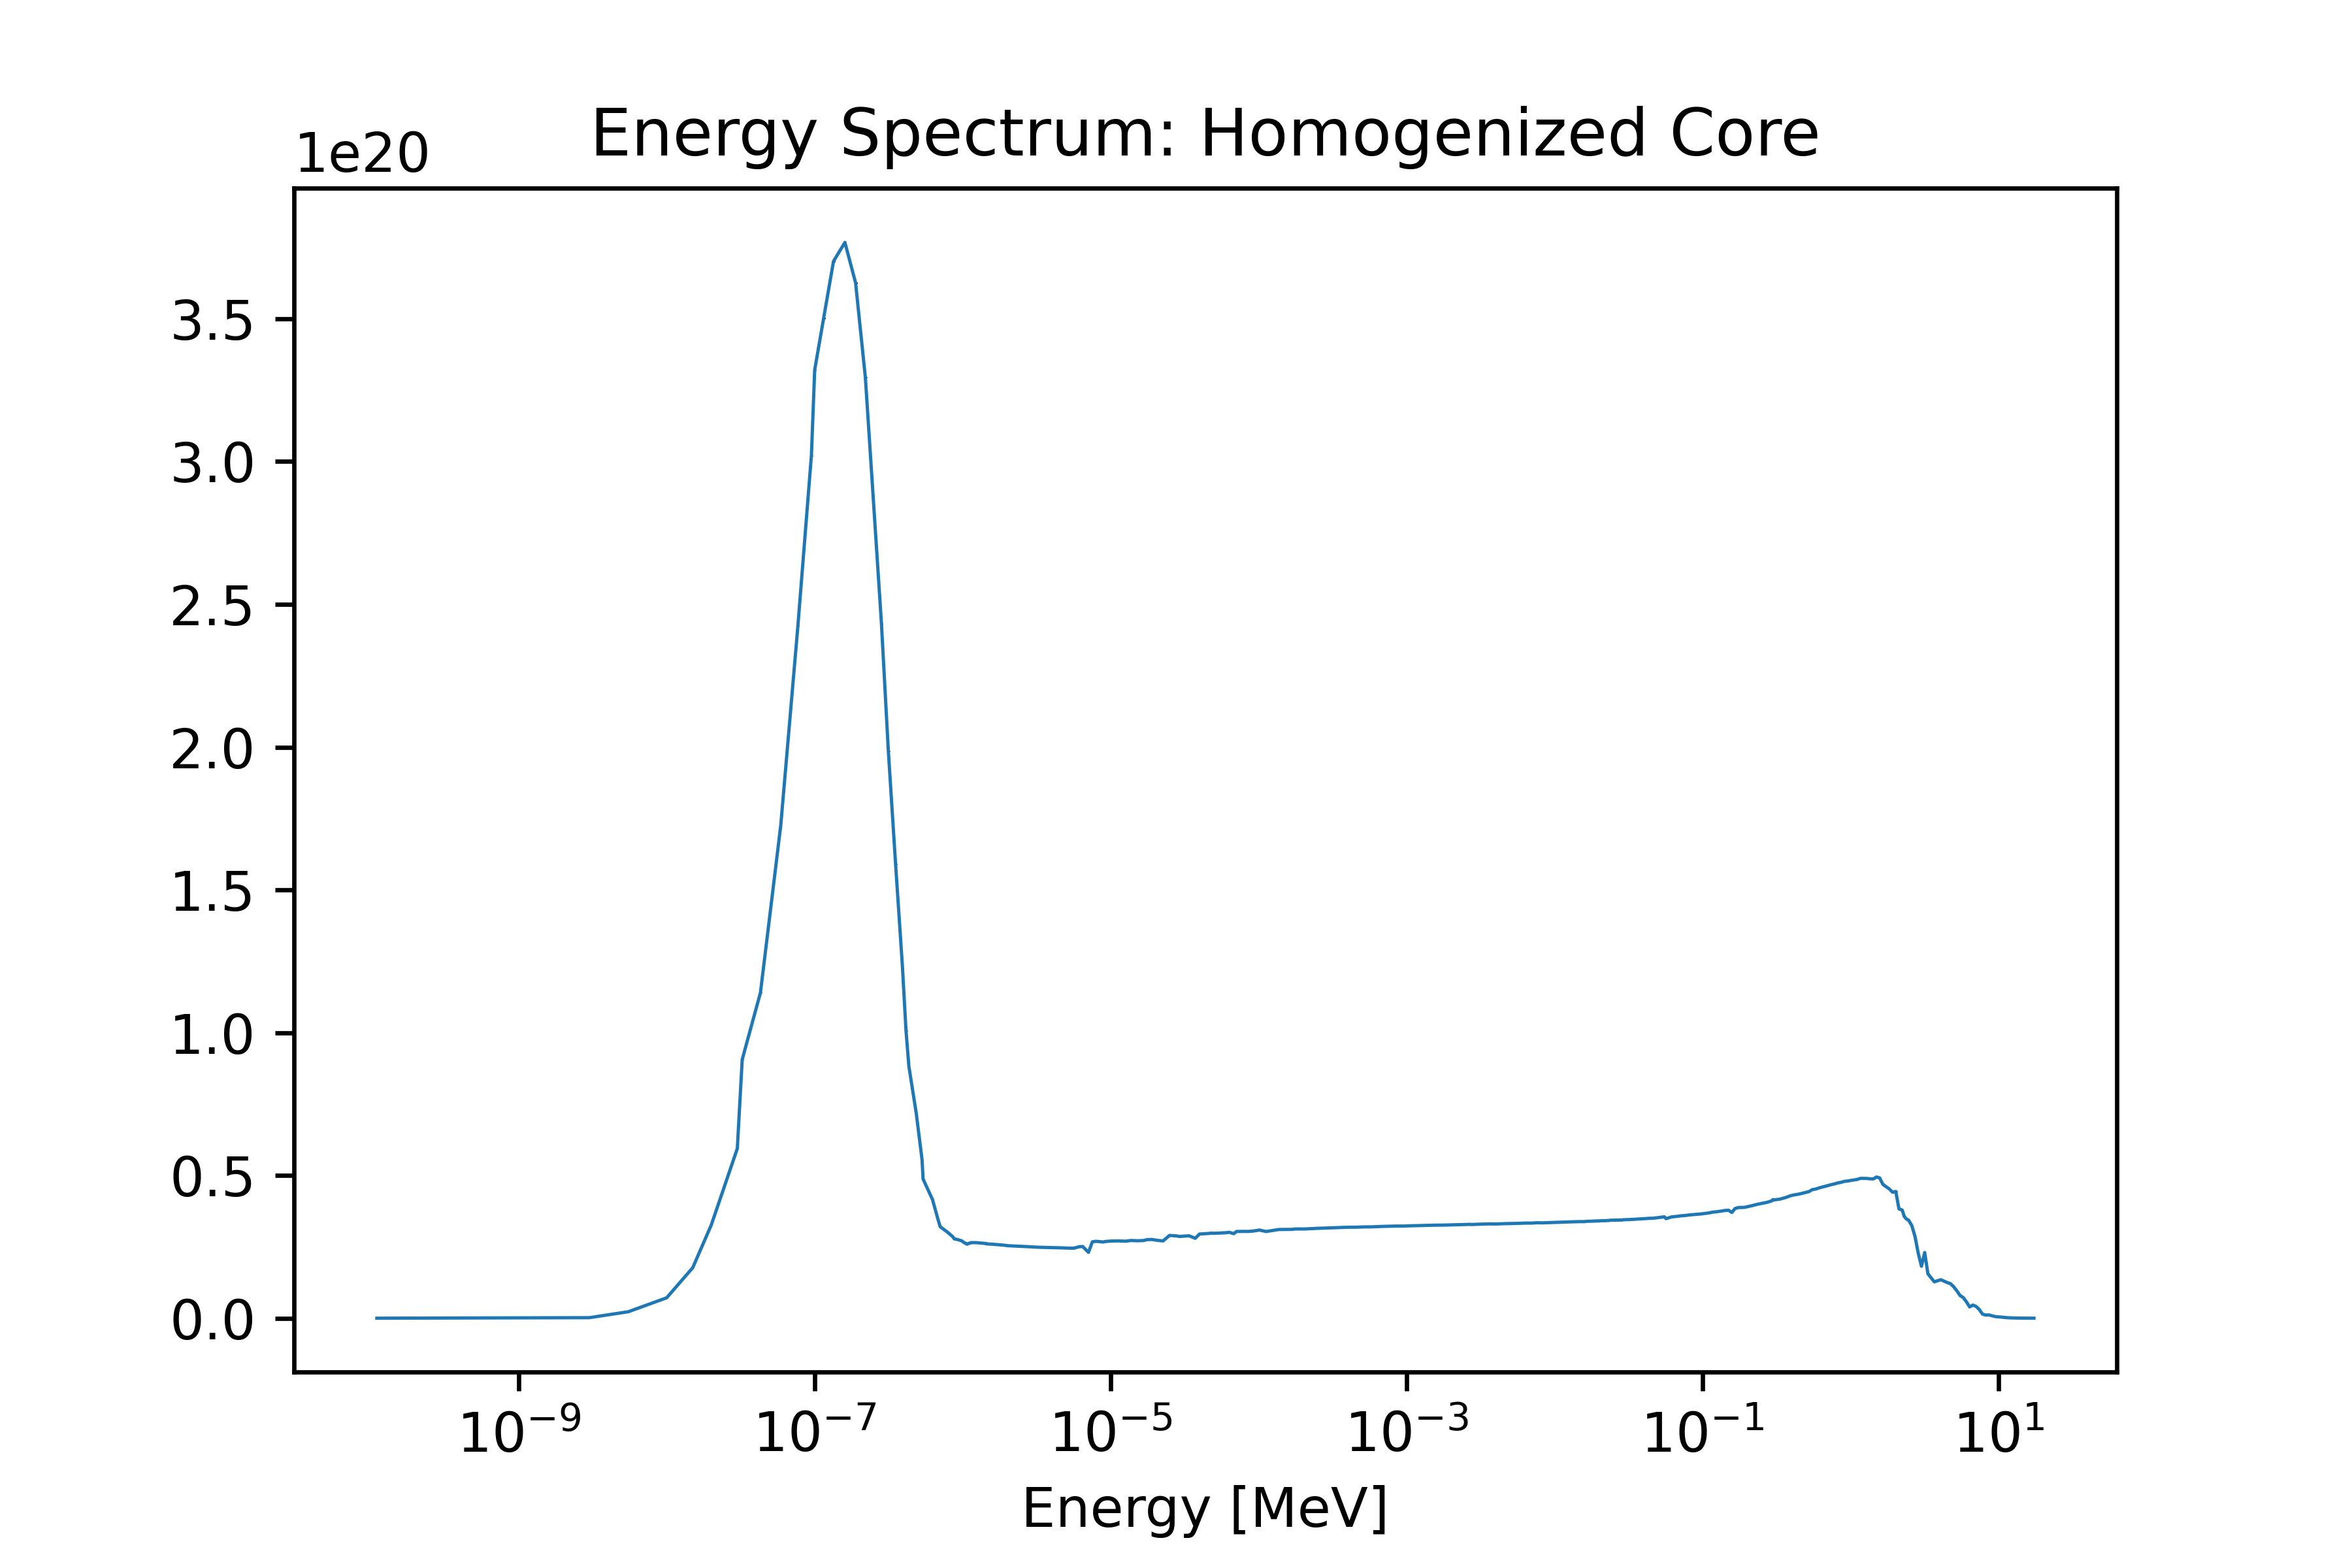
\includegraphics[width=0.95\linewidth]{figures/core_spec_homog}
  \caption{Lethargy Adjusted Neutron Flux Energy Spectrum in the Whole-Core for the Homogenized-Pebble Sangamon20}
  \label{fig:hom-core}
\end{figure}

\begin{figure}[H]
\centering
  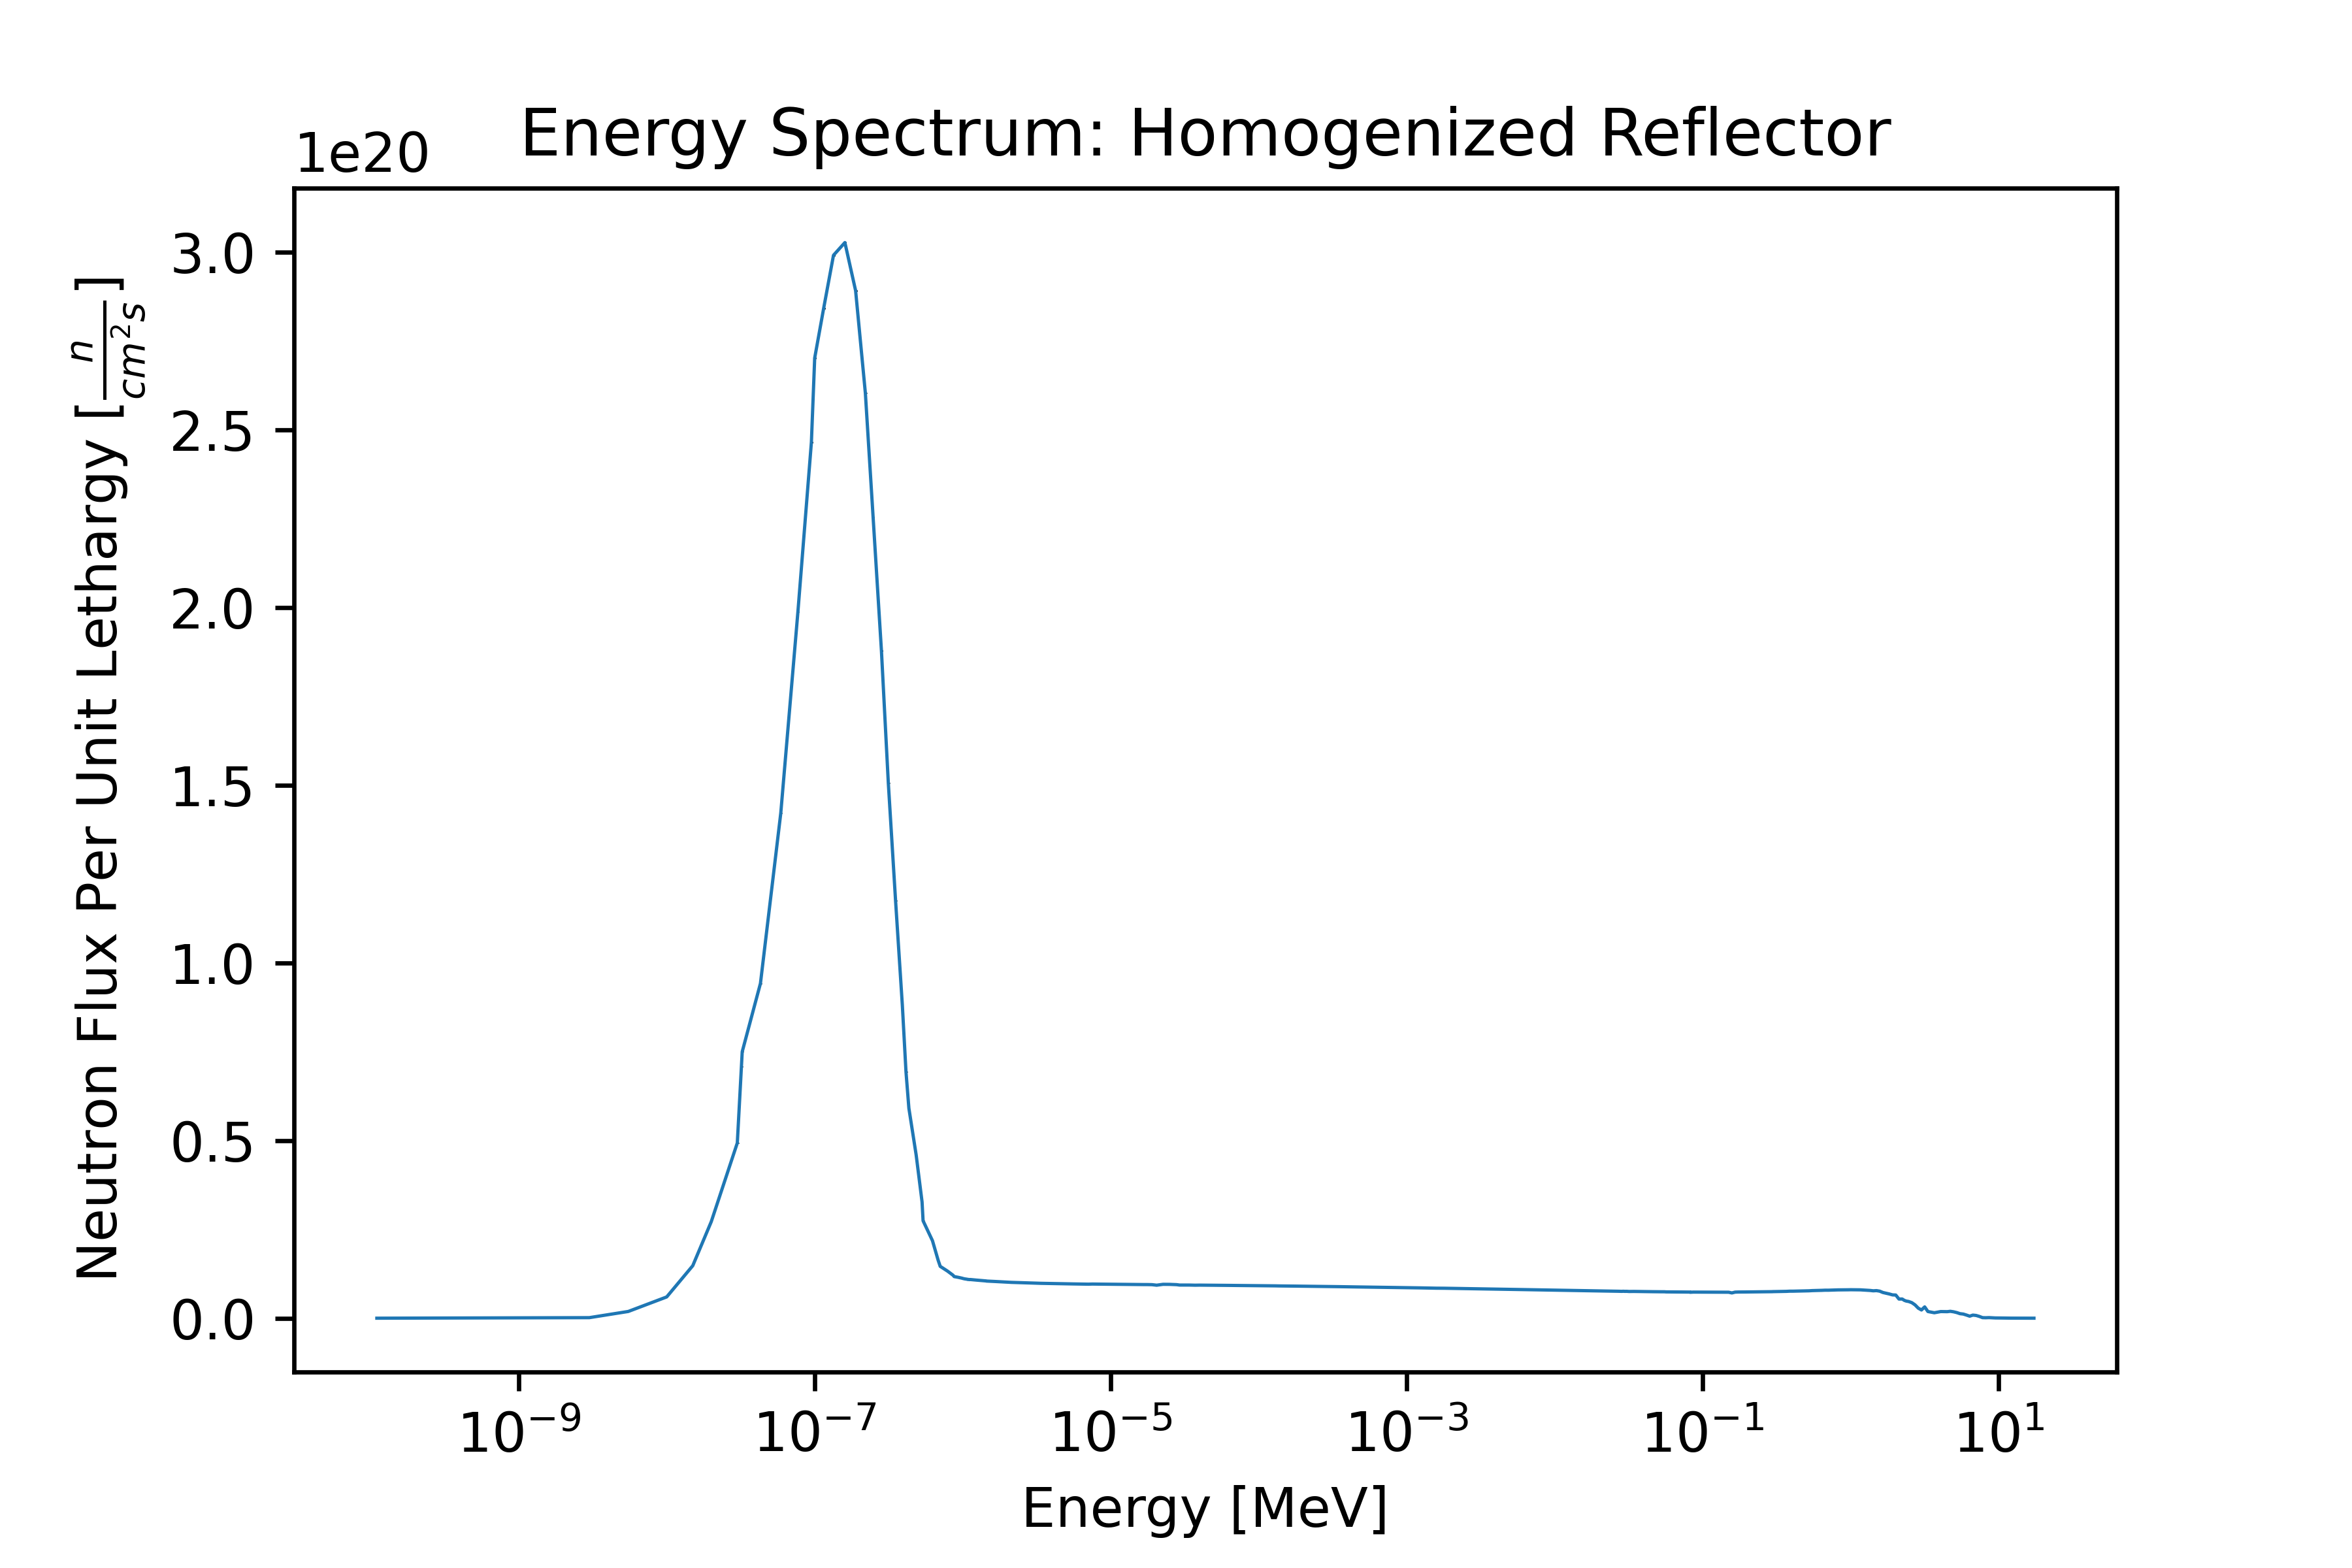
\includegraphics[width=0.95\linewidth]{figures/reflect_spec_homog}
  \caption{Lethargy Adjusted Neutron Flux Energy Spectrum in the Reflector for the Homogenized-Pebble Sangamon20}
  \label{fig:hom-reflec}
\end{figure}


The thermal peak of the whole-core and reflector both occur around $10\times10^{-07}$ MeV, which is also the energy of neutrons most-responsible for fission.  The thermalization of neutrons in the reflector dominates the spectrum in Figure \ref{fig:hom-all}, indicated by the high magnitude of the thermal peak in the reflector and core and their similar shape.

The spectra for a randomly selected fresh and sixth-pass pebble are subject to the highest uncertainty of all the provided spectra in Figure \ref{fig:hom-all}, as a single pebble has a relatively small bin size, which means fewer particles contribute to the tally regions.  However, if plotted alongside the coolant spectra, as in Figure \ref{fig:hom-all}, they provide a clearer look at the flux energy spectrum in the active core region.  We can see that, while the thermal energy of the fresh and six-pass pebbles is similar in shape and magnitude, the magnitude of the faster groups differs considerably.

Figure \ref{fig:hom-peb} shows the spectra of the one, two, three, four, and five pass pebbles, alongside the fresh pebble, six-pass pebble, and coolant spectra from \ref{fig:hom-all}. 

\begin{figure}[H]
\centering
  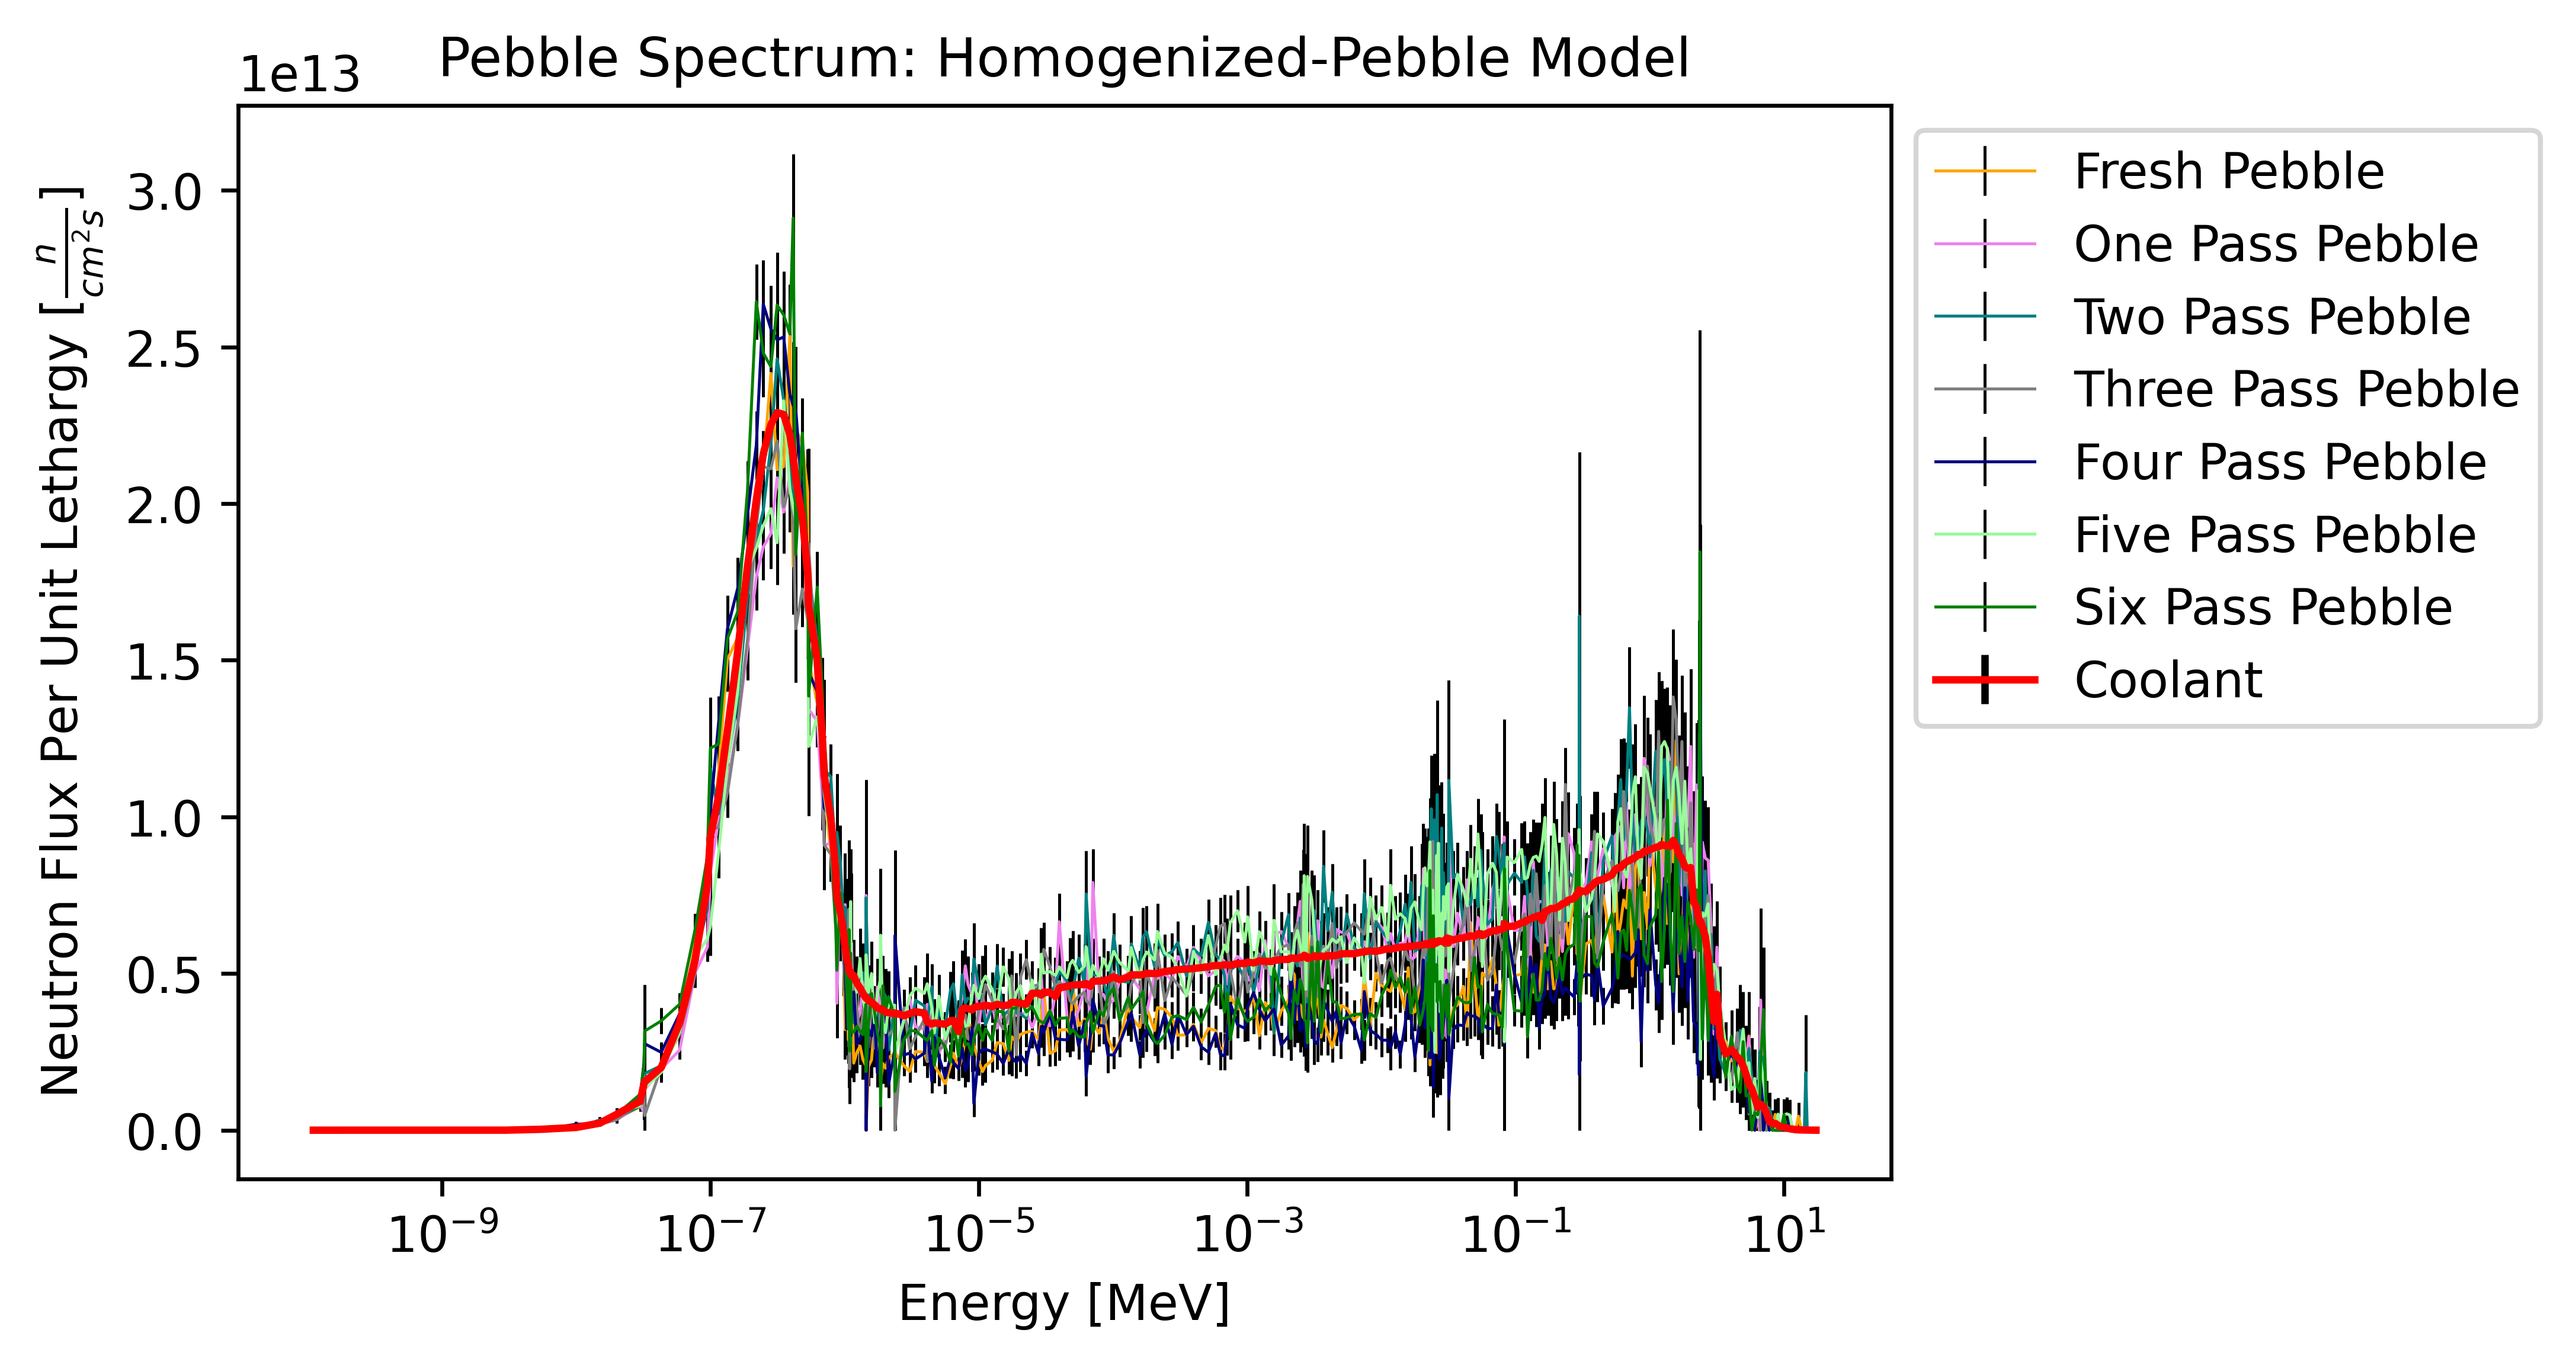
\includegraphics[width=0.95\linewidth]{figures/pebs_spec_homog_er}
  \caption{Lethargy Adjusted Neutron Flux Energy Spectrum in the Each Pebble Burnup and Coolant for the Homogenized-Pebble Sangamon20}
  \label{fig:hom-peb}
\end{figure}


Figure \ref{fig:hom-peb} shows that, compared the other pebble burnup levels, the fresh and six-pass pebbles have the softest spectra.  This may be due to the higher levels of $^{239}Pu$ in the \acrshort{mol} pebbles. Additionally, once all pebble spectra are presented together, along with the coolant, one can see much more clearly that the coolant spectrum provides a very generalized look at the overall behavior in the pebble spectra.


\section{Effect of Homogenization}
\label{res-hom}

The results discussed in \autoref{res-control} use the assumption of a pebble that has the TRISO particles homogenized and blended with the rest of the pebble matrix in the region containing fuel.  However, homogenization can cause under-predictions of k-eff as much as 5-6\% \cite{brown_stochastic_2005}.  To test the impact of homogenization on Sangamon20, the heterogenization tests were performed.  These tests use an otherwise identical Sangamon20 model with explicitly modeled TRISO particles and compares $k_{eff}$, the core spectra, and the outer reflector current.  As a reminder, the isotopic compositions come from the same burnup simulation.  As such, the isotopic compositions between the homogenized and heterogenized simulations are identical.


\begin{figure}[H]
\centering

\begin{subfigure}{0.45\textwidth}
  \includegraphics[width=0.95\linewidth]{figures/het/het-r}
  \caption{Radial Cross Section at y=0}
  \label{fig:heta}
\end{subfigure}%
%
\begin{subfigure}{0.45\textwidth}
  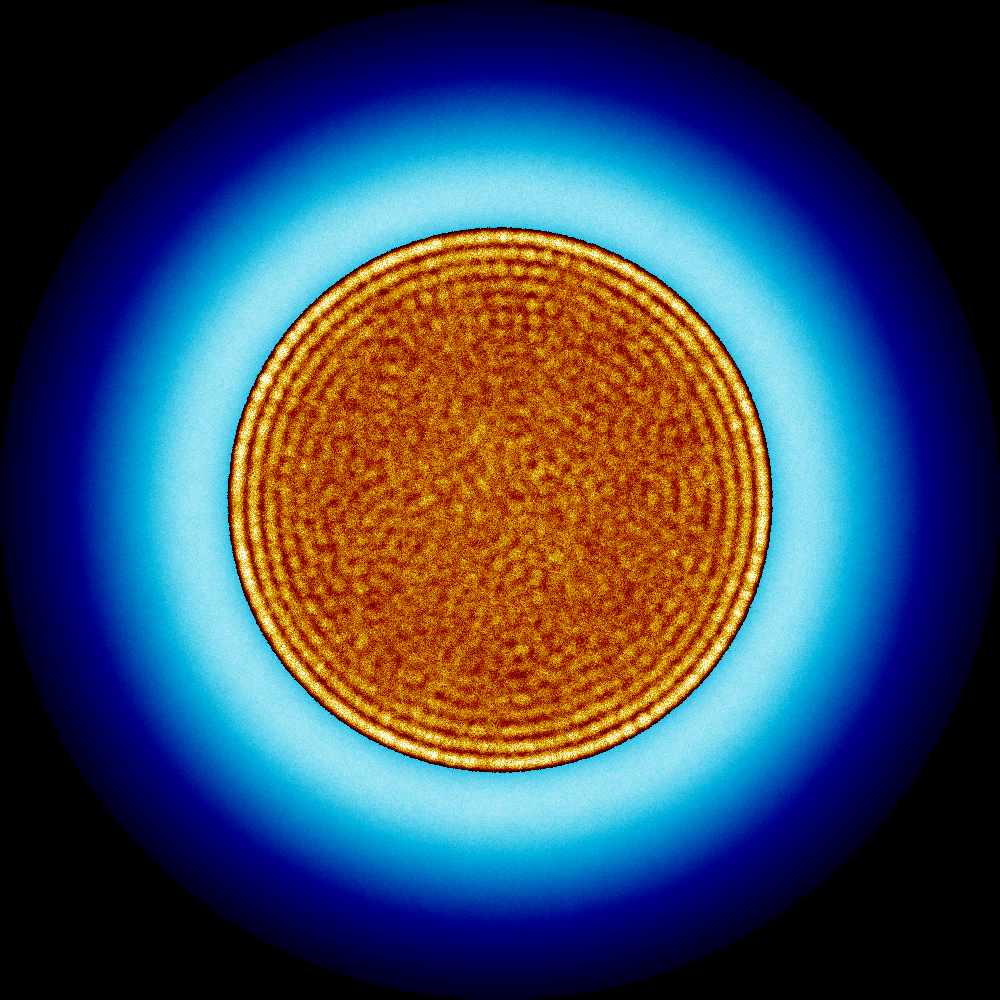
\includegraphics[width=0.95\linewidth]{figures/het/het-rm}
  \caption{Radial Mesh}
  \label{fig:hetb}
\end{subfigure}

\begin{subfigure}{0.45\textwidth}
  \includegraphics[width=0.95\linewidth]{figures/het/het-v}
  \caption{Axial Cross Section at z=0 }
  \label{fig:hetc}
\end{subfigure}
%
\begin{subfigure}{0.45\textwidth}
  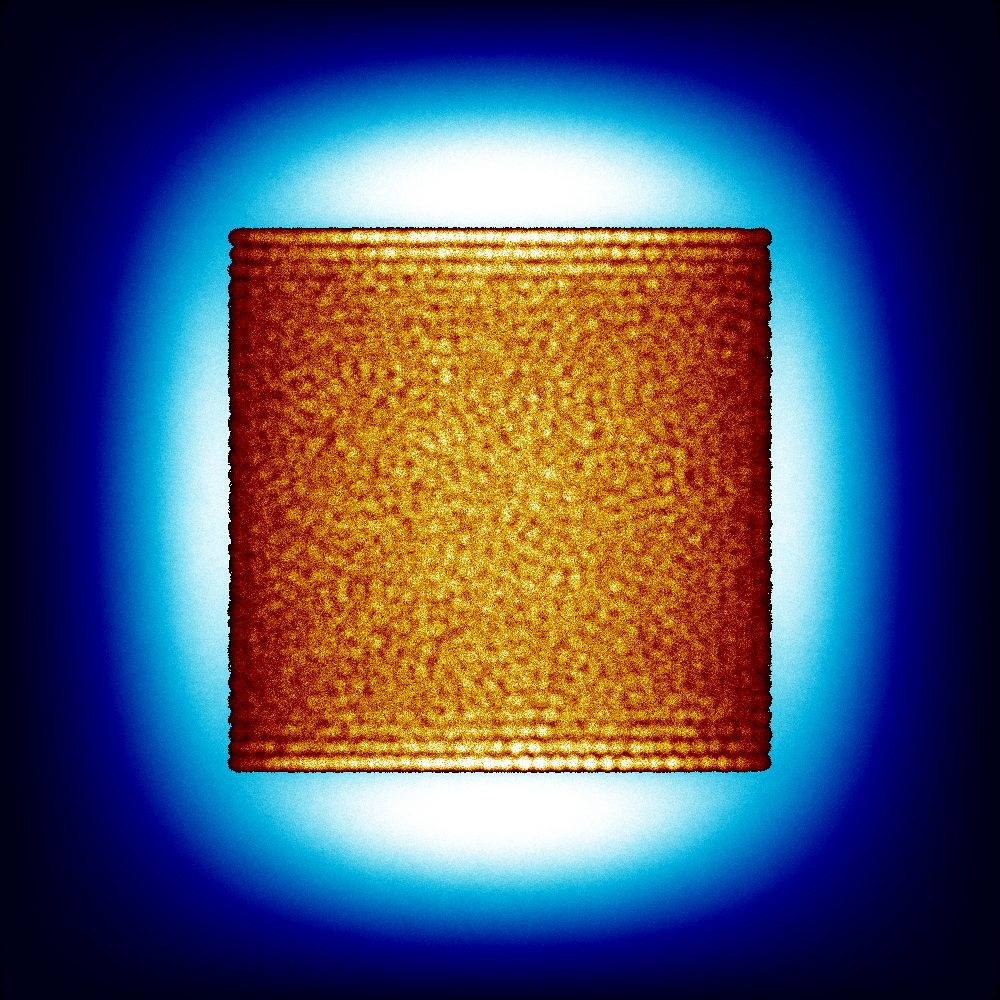
\includegraphics[width=0.95\linewidth]{figures/het/het-vm}
  \caption{Axial Mesh}
  \label{fig:hetd}
\end{subfigure}
%
\caption{Full Core Using Heterogenized Pebbles}
\label{fig:het}
\end{figure}

The heterogenized-TRISO model reported a $k_{eff}$ of $1.056 \pm 0.00033$.  This is significantly higher than the $k_{eff}$ reported for the control (homogenized-TRISO) model --- only $1.009 \pm 0.00055$.  In agreement with \cite{brown_stochastic_2005}, this is a difference of 4.45\%.  

In \ref{fig:het}, we can observe the axial and radial fission rates and thermal fluxes of the heterogeneous core.  Overall, the mesh result for the heterogenization test fission rate is much the same - the banding patterns are still present, if slightly less defined.  In \ref{table:cpu-params} below, the run time and CPU usage parameters are provided.  CPU usage is defined as the ratio of CPU time to total run time.

\begin{table}[h!]
\centering
\caption{Runtime and CPU Usage Between the Homogenized and Heterogenized Sangamon20 Models}
\begin{tabular}{ c  c  c  c }
\hline
Model & Total CPU Time $\left[ minutes \right]$ & Running Time $\left[ minutes \right]$ & CPU Usage \\
\hline
Homogeneous Pebbles & 615.61 & 273.83 & 2.24815  \\
Heterogeneous Pebbles & 915.96 & 240.75 & 3.80461 \\
\hline
\end{tabular}

\label{table:cpu-params}
\end{table}

Even though the homogeneous model had a run time that was around 30 minutes longer, it took significantly less CPU time than the heterogeneous model.  It is possible that this difference in total run time doesn't occur on average, but more runs are required to test this.

While Figure \ref{fig:het} best serves as a qualitative visualization aid, Figures \ref{fig:het-det-xy}, \ref{fig:het-det-z}, \ref{fig:het-plane-therm}, and \ref{fig:het-plane-fast} support this in a more quantitative manner.  These figures provide the shape and magnitude of the fluxes.


\begin{figure}[H]
\centering

\begin{subfigure}{0.9\textwidth}
  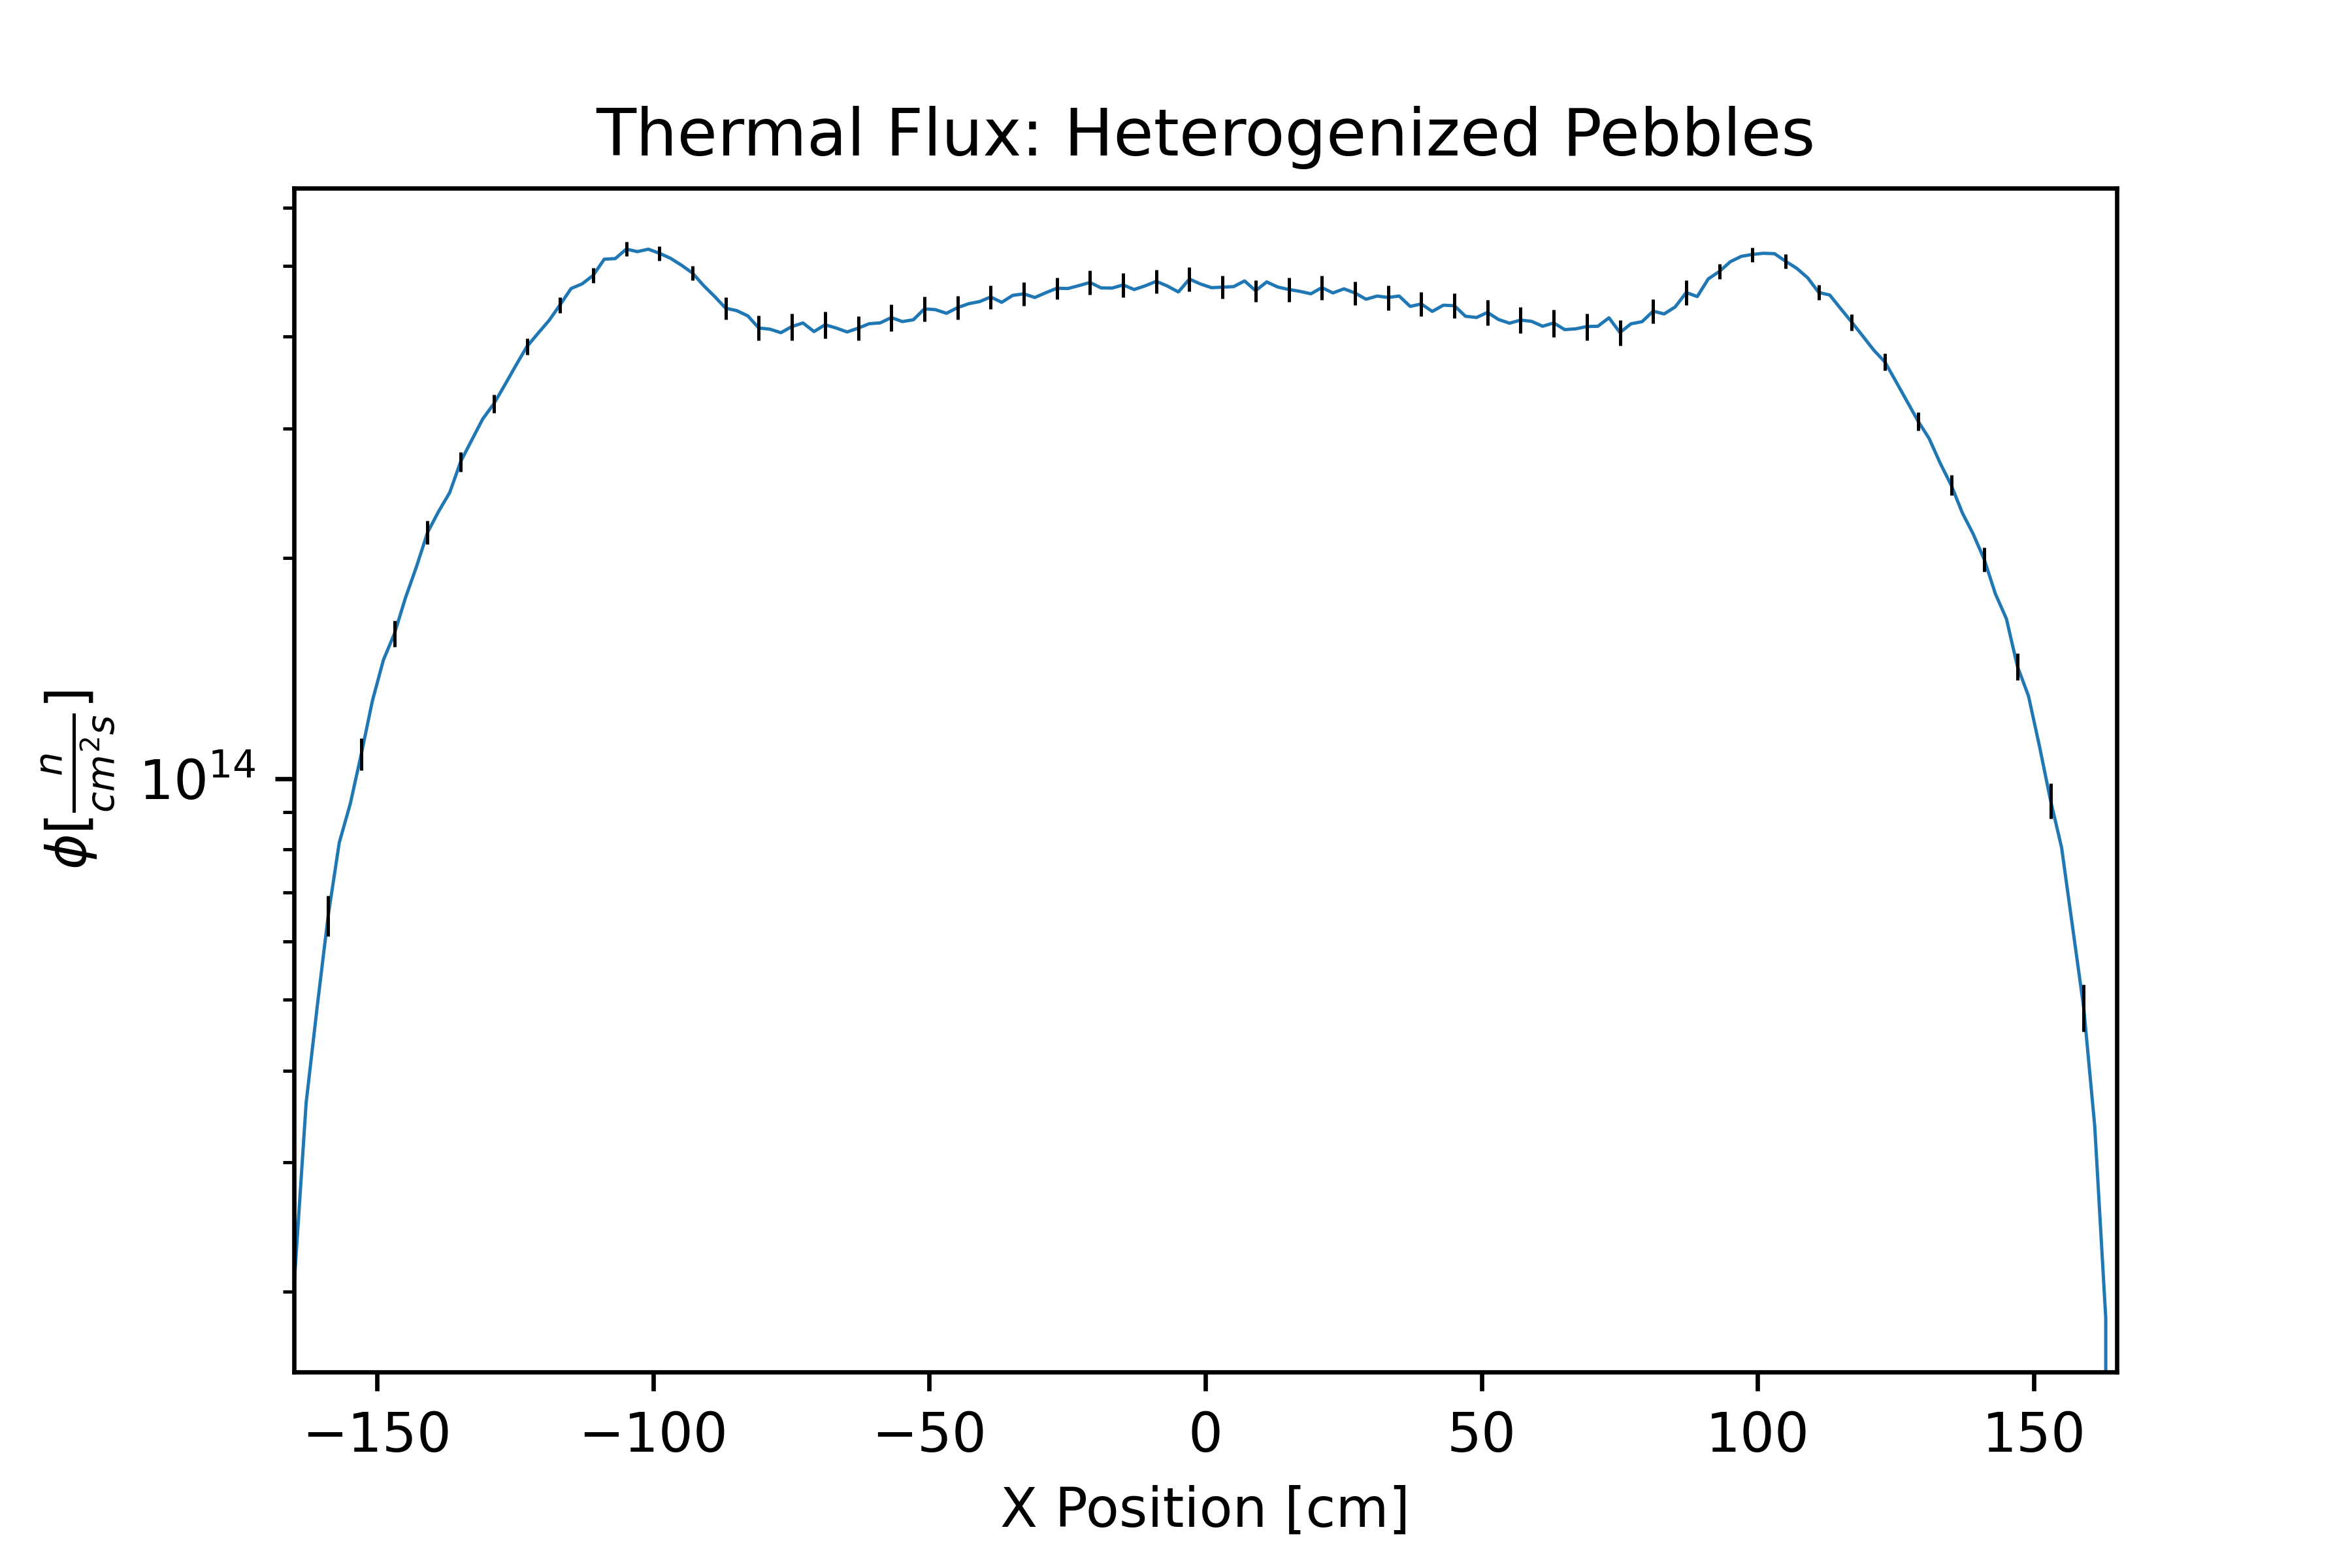
\includegraphics[width=0.95\linewidth]{figures/therm_flux_het.png}
  \caption{Thermal Flux}
  \label{fig:het-det-xy-therm}
\end{subfigure}%

\caption{Radial Thermal and Fast Flux Profiles: Heterogenized Pebbles}
\end{figure}

\begin{figure}[H]\ContinuedFloat
\centering

\begin{subfigure}{0.9\textwidth}
  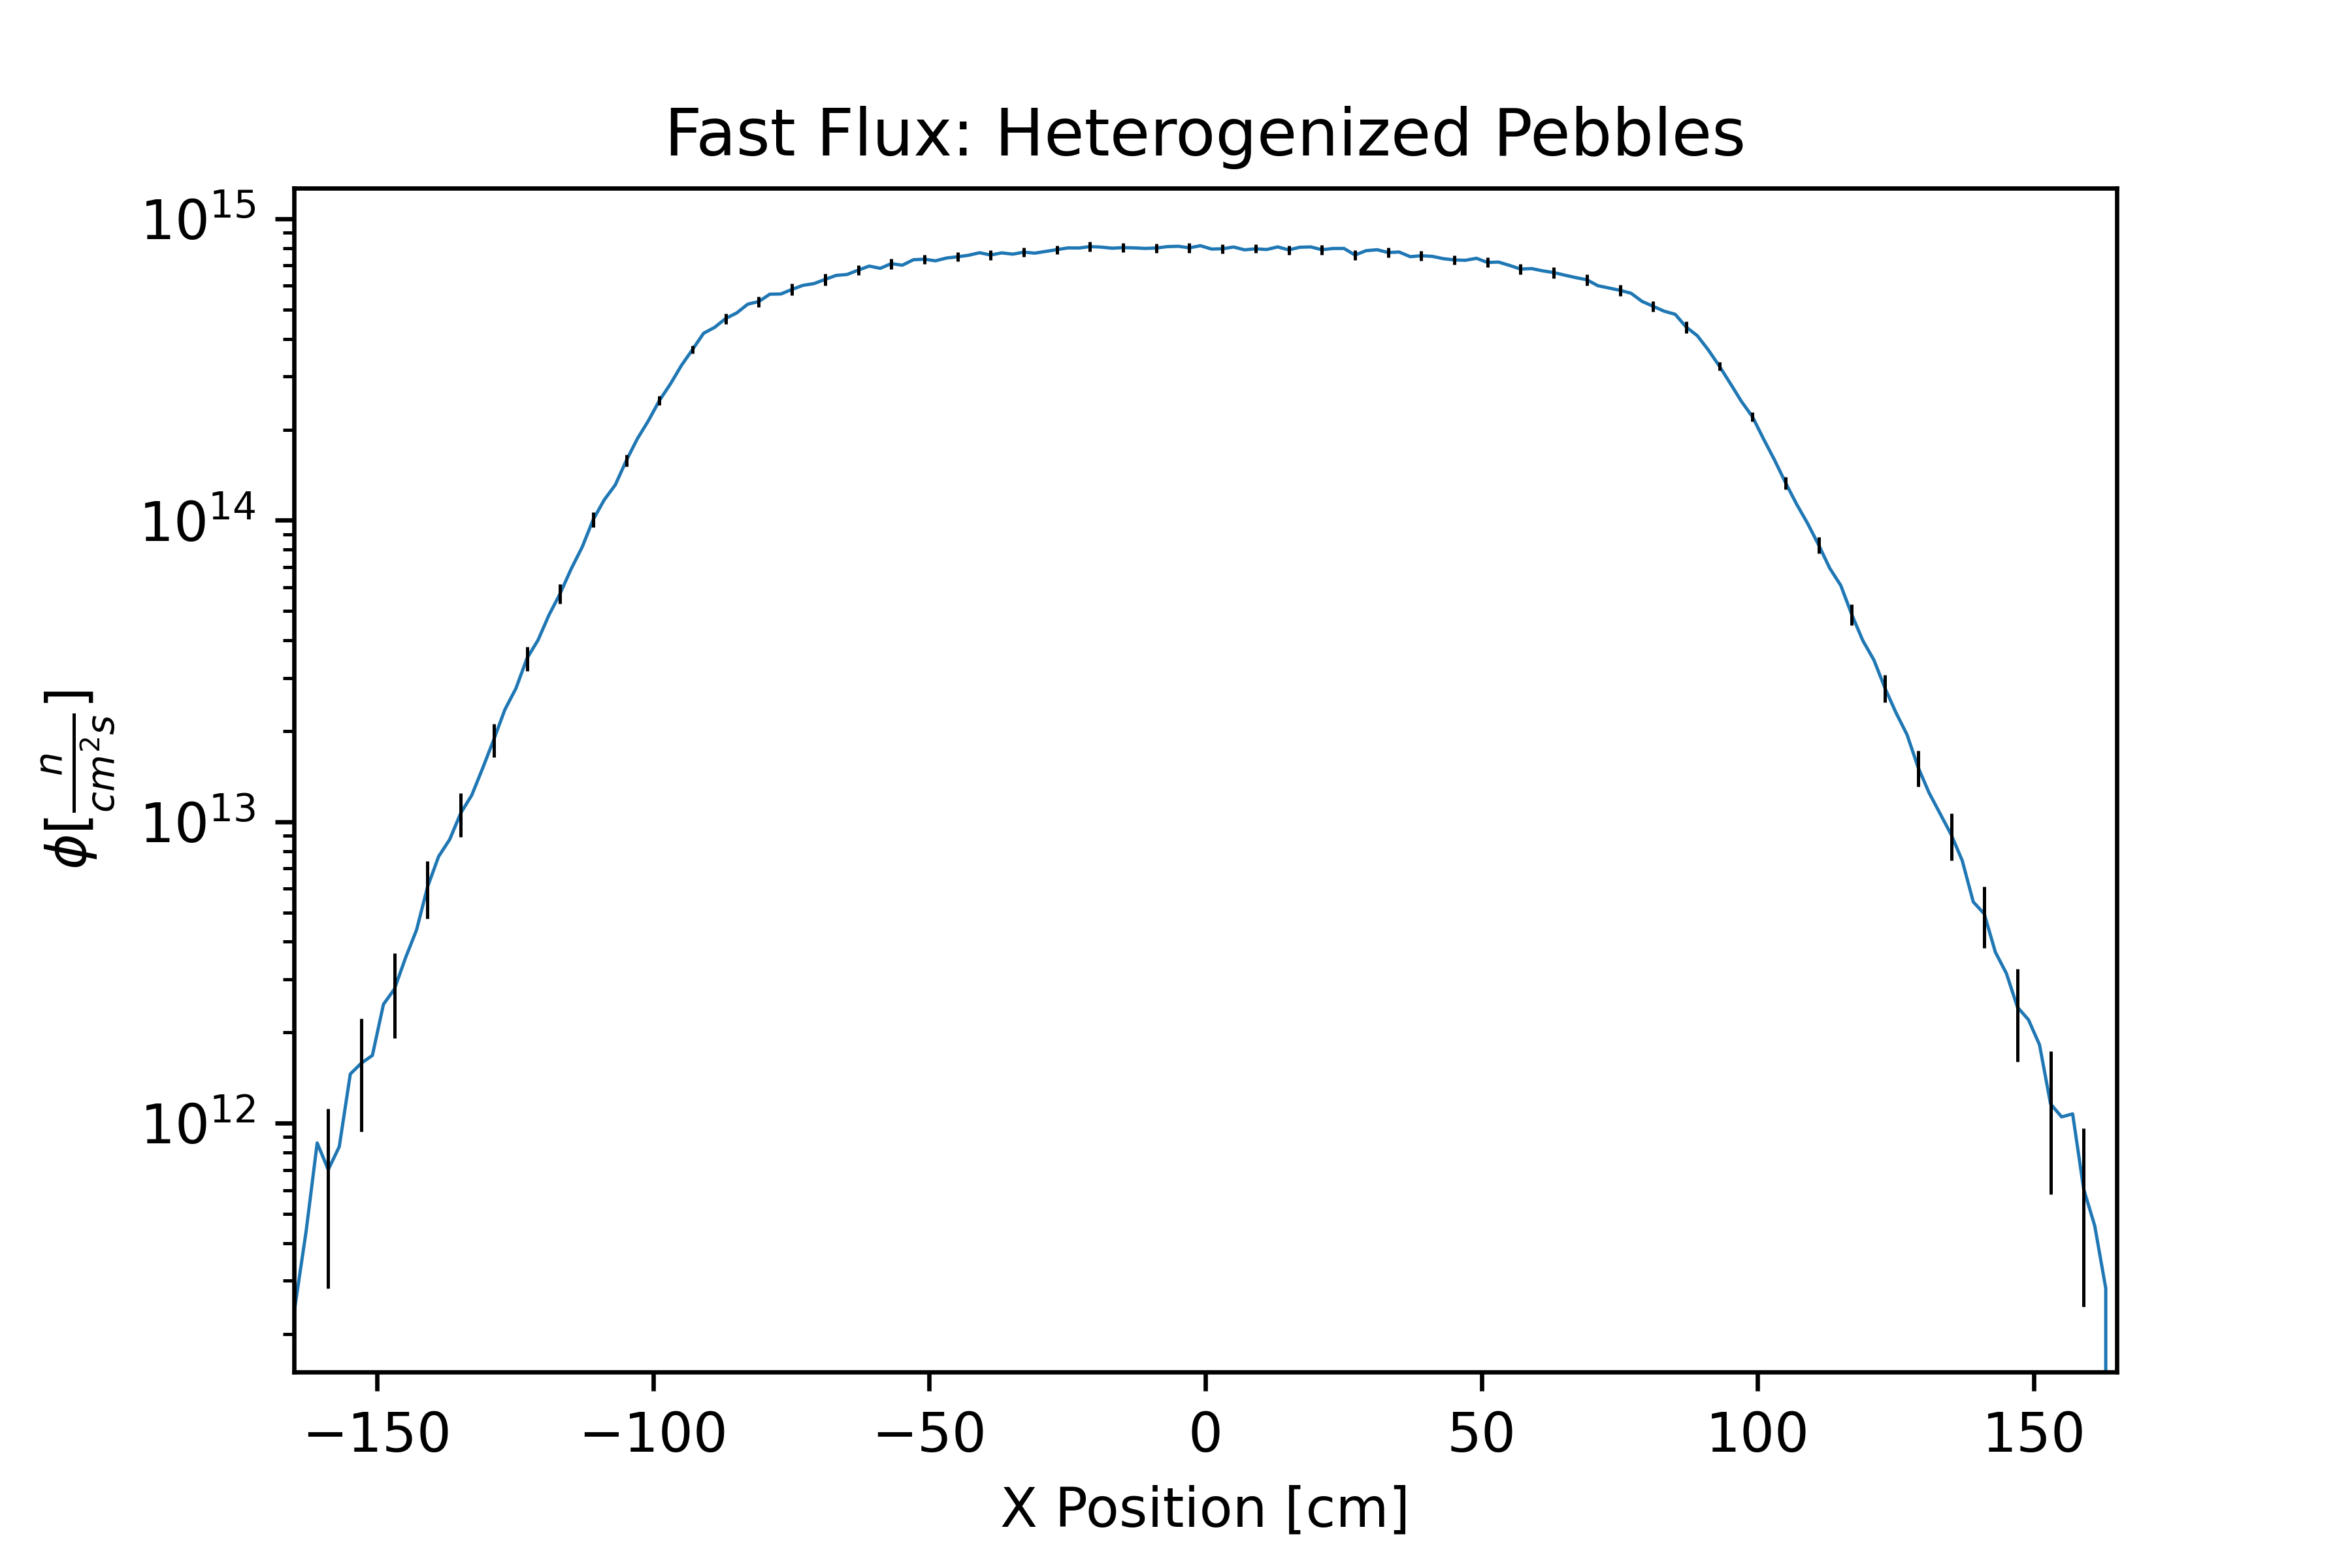
\includegraphics[width=0.95\linewidth]{figures/fast_flux_het.png}
  \caption{Fast Flux}
  \label{fig:het-det-xy-fast}
\end{subfigure}


\caption{Radial Thermal and Fast Flux Profiles: Heterogenized Pebbles (cont.)}
\label{fig:het-det-xy}
\end{figure}

Compared with the homogenized Sangamon20, the heterogenized core reports a slightly lower neutron current at the outer edge of the reflector, at $6.809\times10^{11} \pm 5.515\times10^{08}$, a relative difference of 2.85\%.  The heterogenized model otherwise shows a similar flux profile to the homogenized model (see Figure \ref{fig:diff-flux}), and experiences a similar level of uncertainty in the outer edges of the reflector for the fast flux profiles, likely due to the significant thermalization of neutrons by that point in the reflector --- which results in fewer fast neutrons contributing to outer region tallies.


\begin{figure}[H]
\centering

  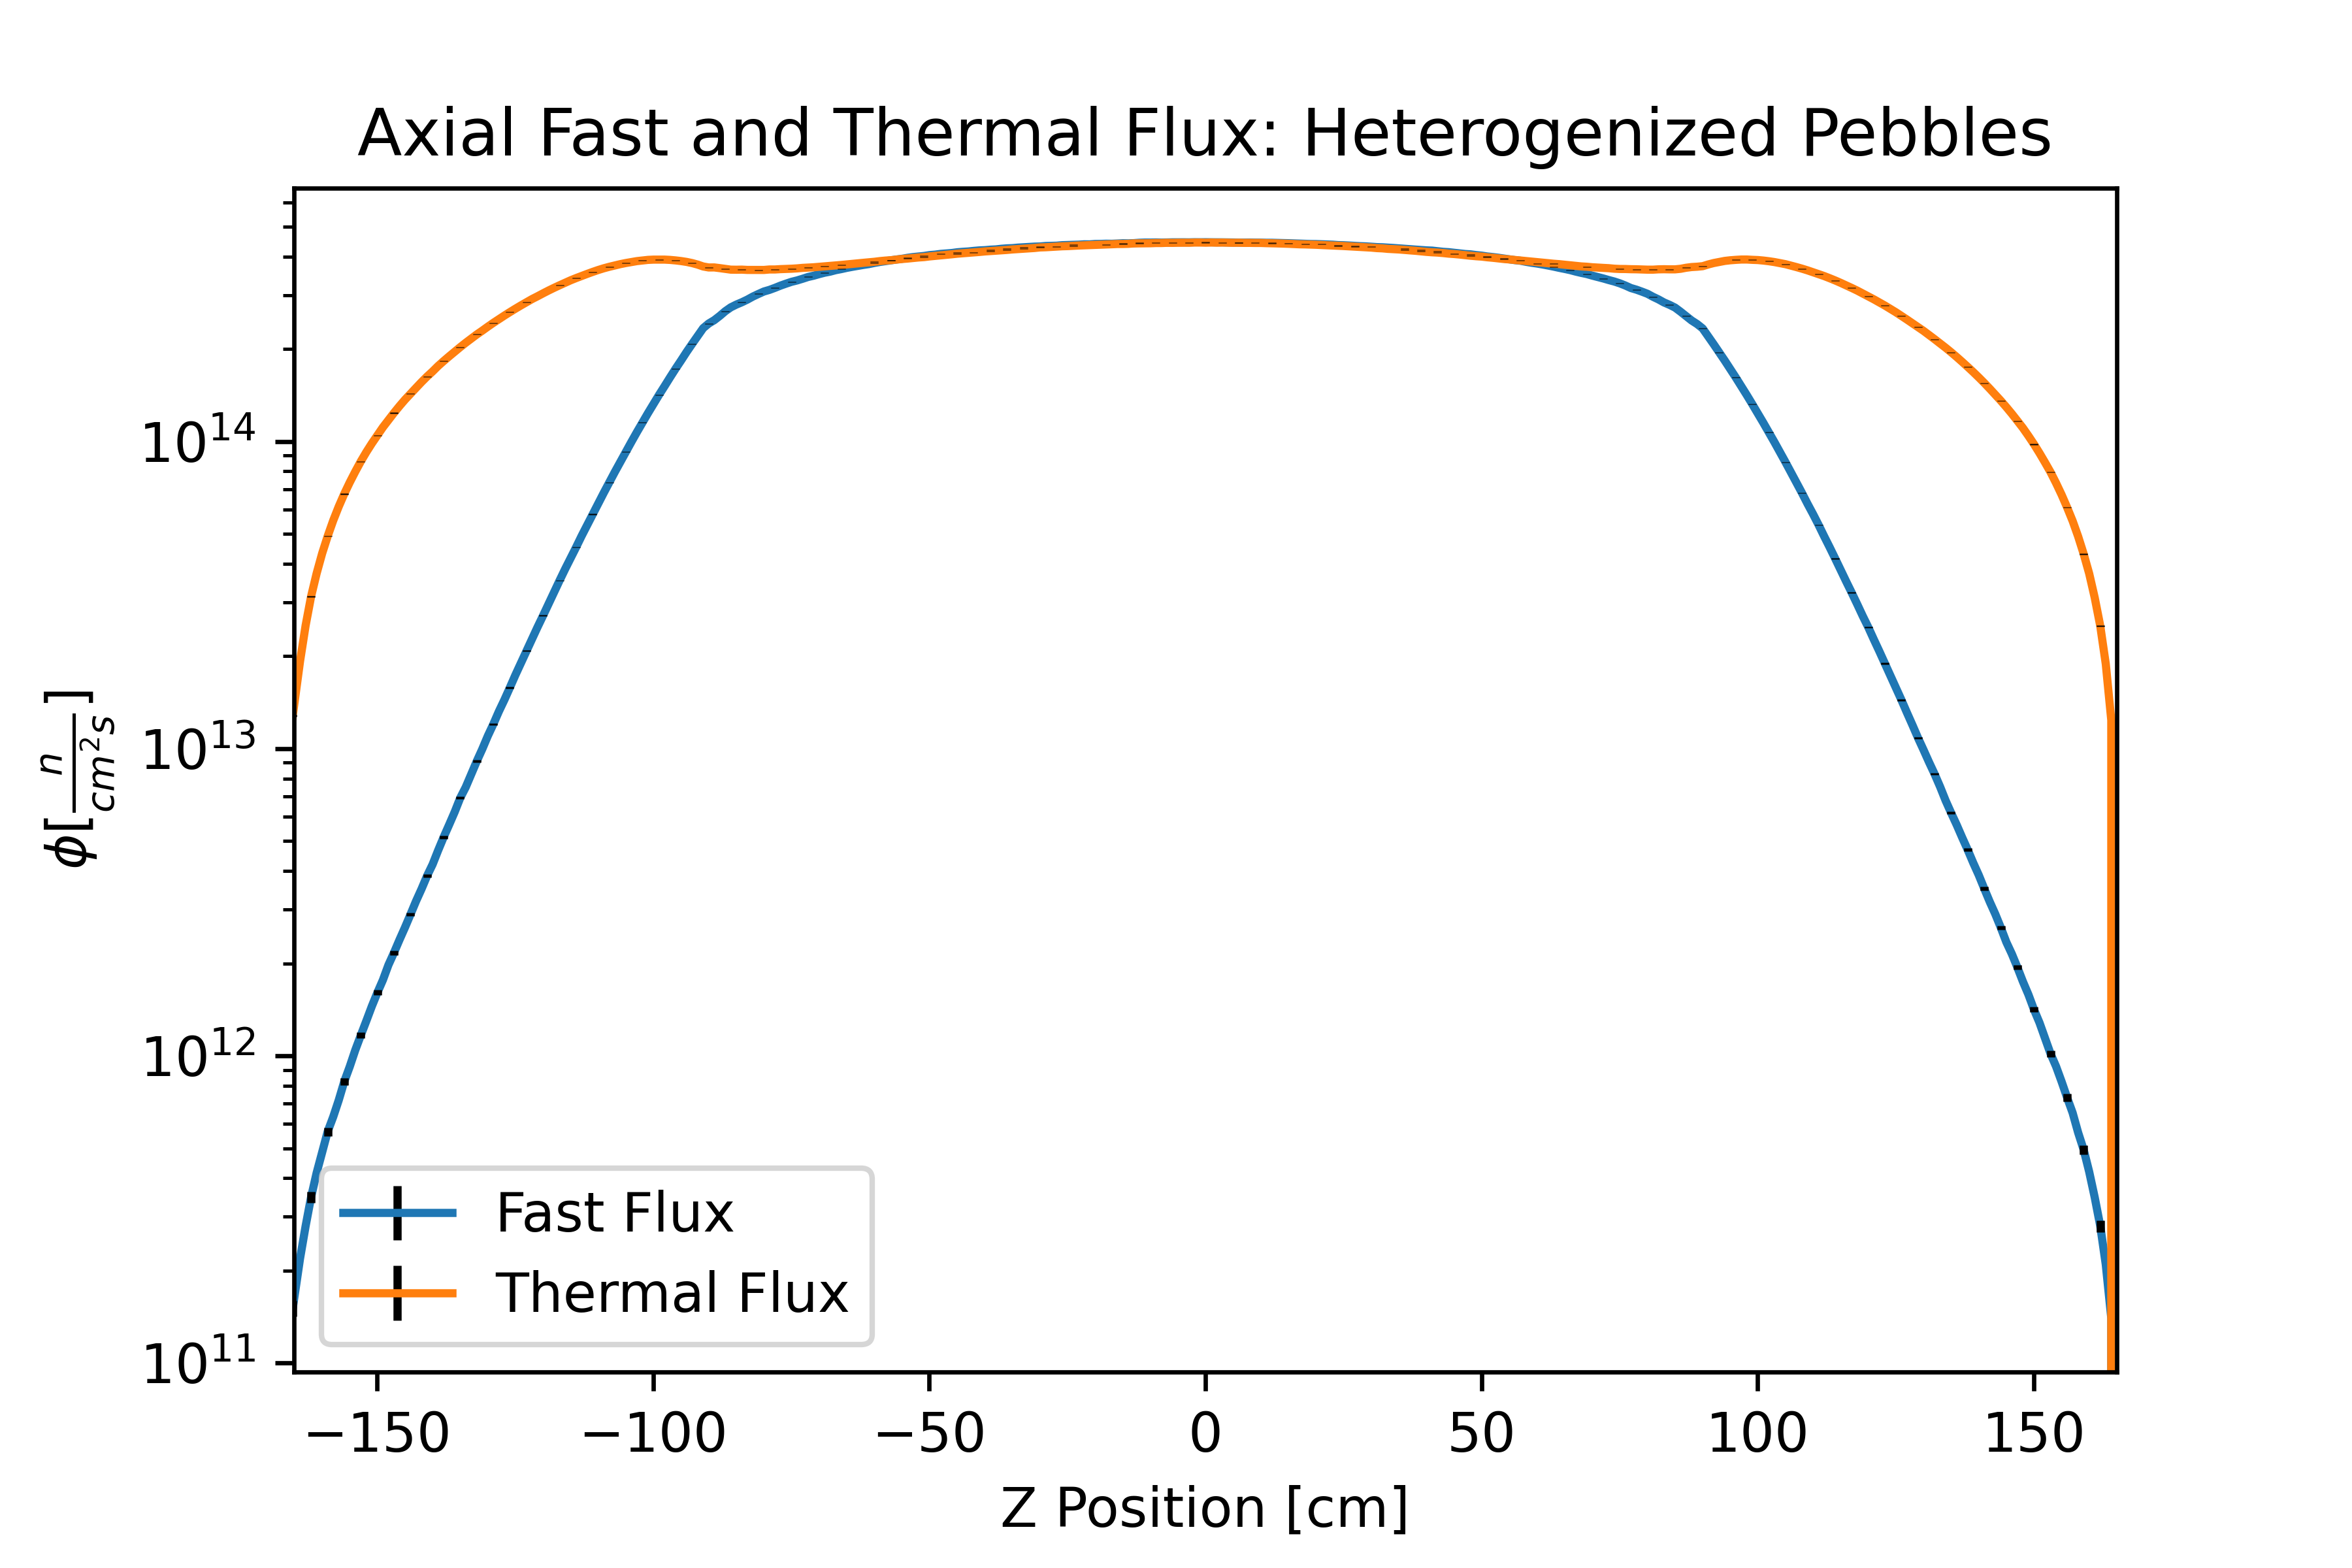
\includegraphics[width=0.95\linewidth]{figures/fast_therm_flux_het_z.png}

\caption{Axial Thermal and Fast Flux Profiles along the Centerline in Sangamon20: Heterogenized Pebbles}
\label{fig:het-det-z}
\end{figure}


\begin{figure}[H]
\centering


\includegraphics[width=0.95\linewidth]{figures/therm_xy_plane_het_er.png}
\caption{Thermal Flux in xy Plane in Sangamon20: Heterogenized Pebbles.  The dotted line annotation marks the boundary between the active core and the graphite reflector.}
\label{fig:het-plane-therm}

\end{figure}

\begin{figure}[H]
\centering

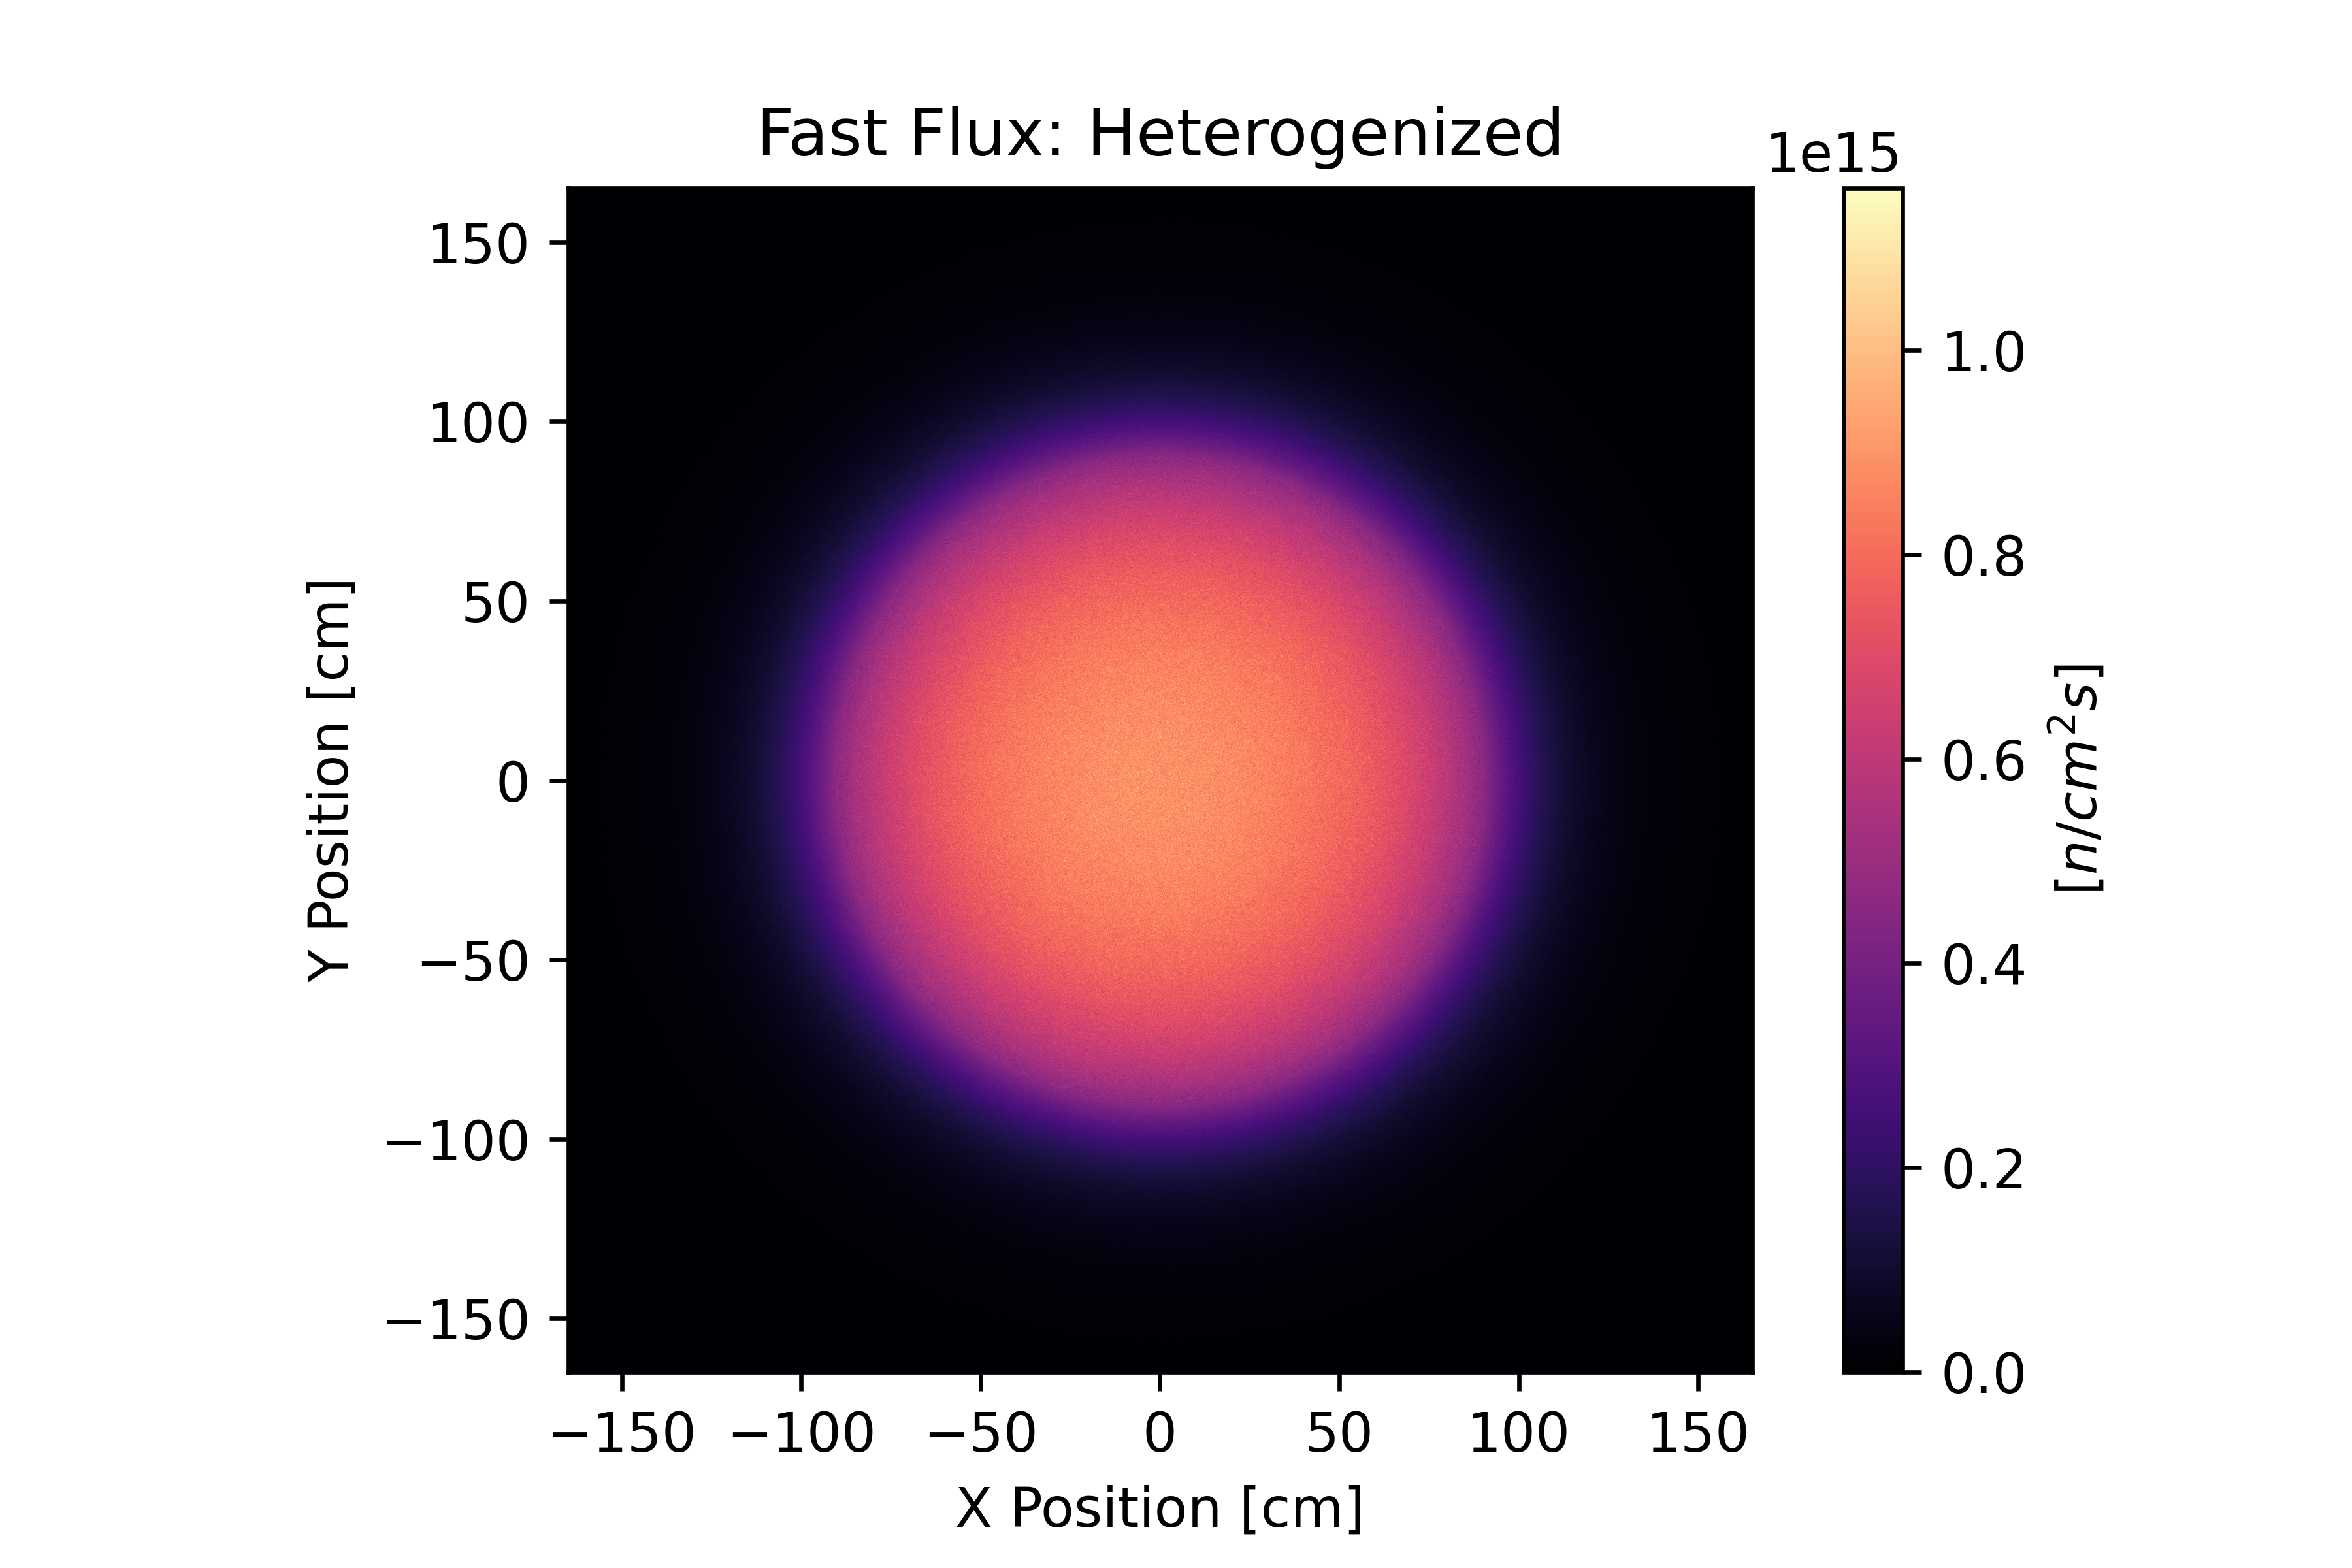
\includegraphics[width=0.95\linewidth]{figures/fast_xy_plane_het_er.png}
\caption{Fast Flux in xy Plane in Sangamon20: Heterogenized Pebbles.  The dotted line annotation marks the boundary between the active core and the graphite reflector.}
\label{fig:het-plane-fast}

\end{figure}

Compared with Figures  \ref{fig:het-plane-therm} and \ref{fig:het-plane-fast}, the edge pebble bands are much less distinct.  This is because the homogenized pebbles have the fissile material spread over the entirety of the 2.5 cm radius fueled center.  The heterogenized pebbles, meanwhile, may have the same number of fissile atoms, but they concentrate the regions capable of fission in the TRISO kernel.  The rest of the pebble consists of its graphite matrix.  This results in a self-shielding effect.  Because the fission reactions are not localized to the TRISO kernels, the entire fuel region is more clearly-defined visually in the homogeneous results.


\begin{figure}[H]
\centering

\begin{subfigure}{0.95\textwidth}
  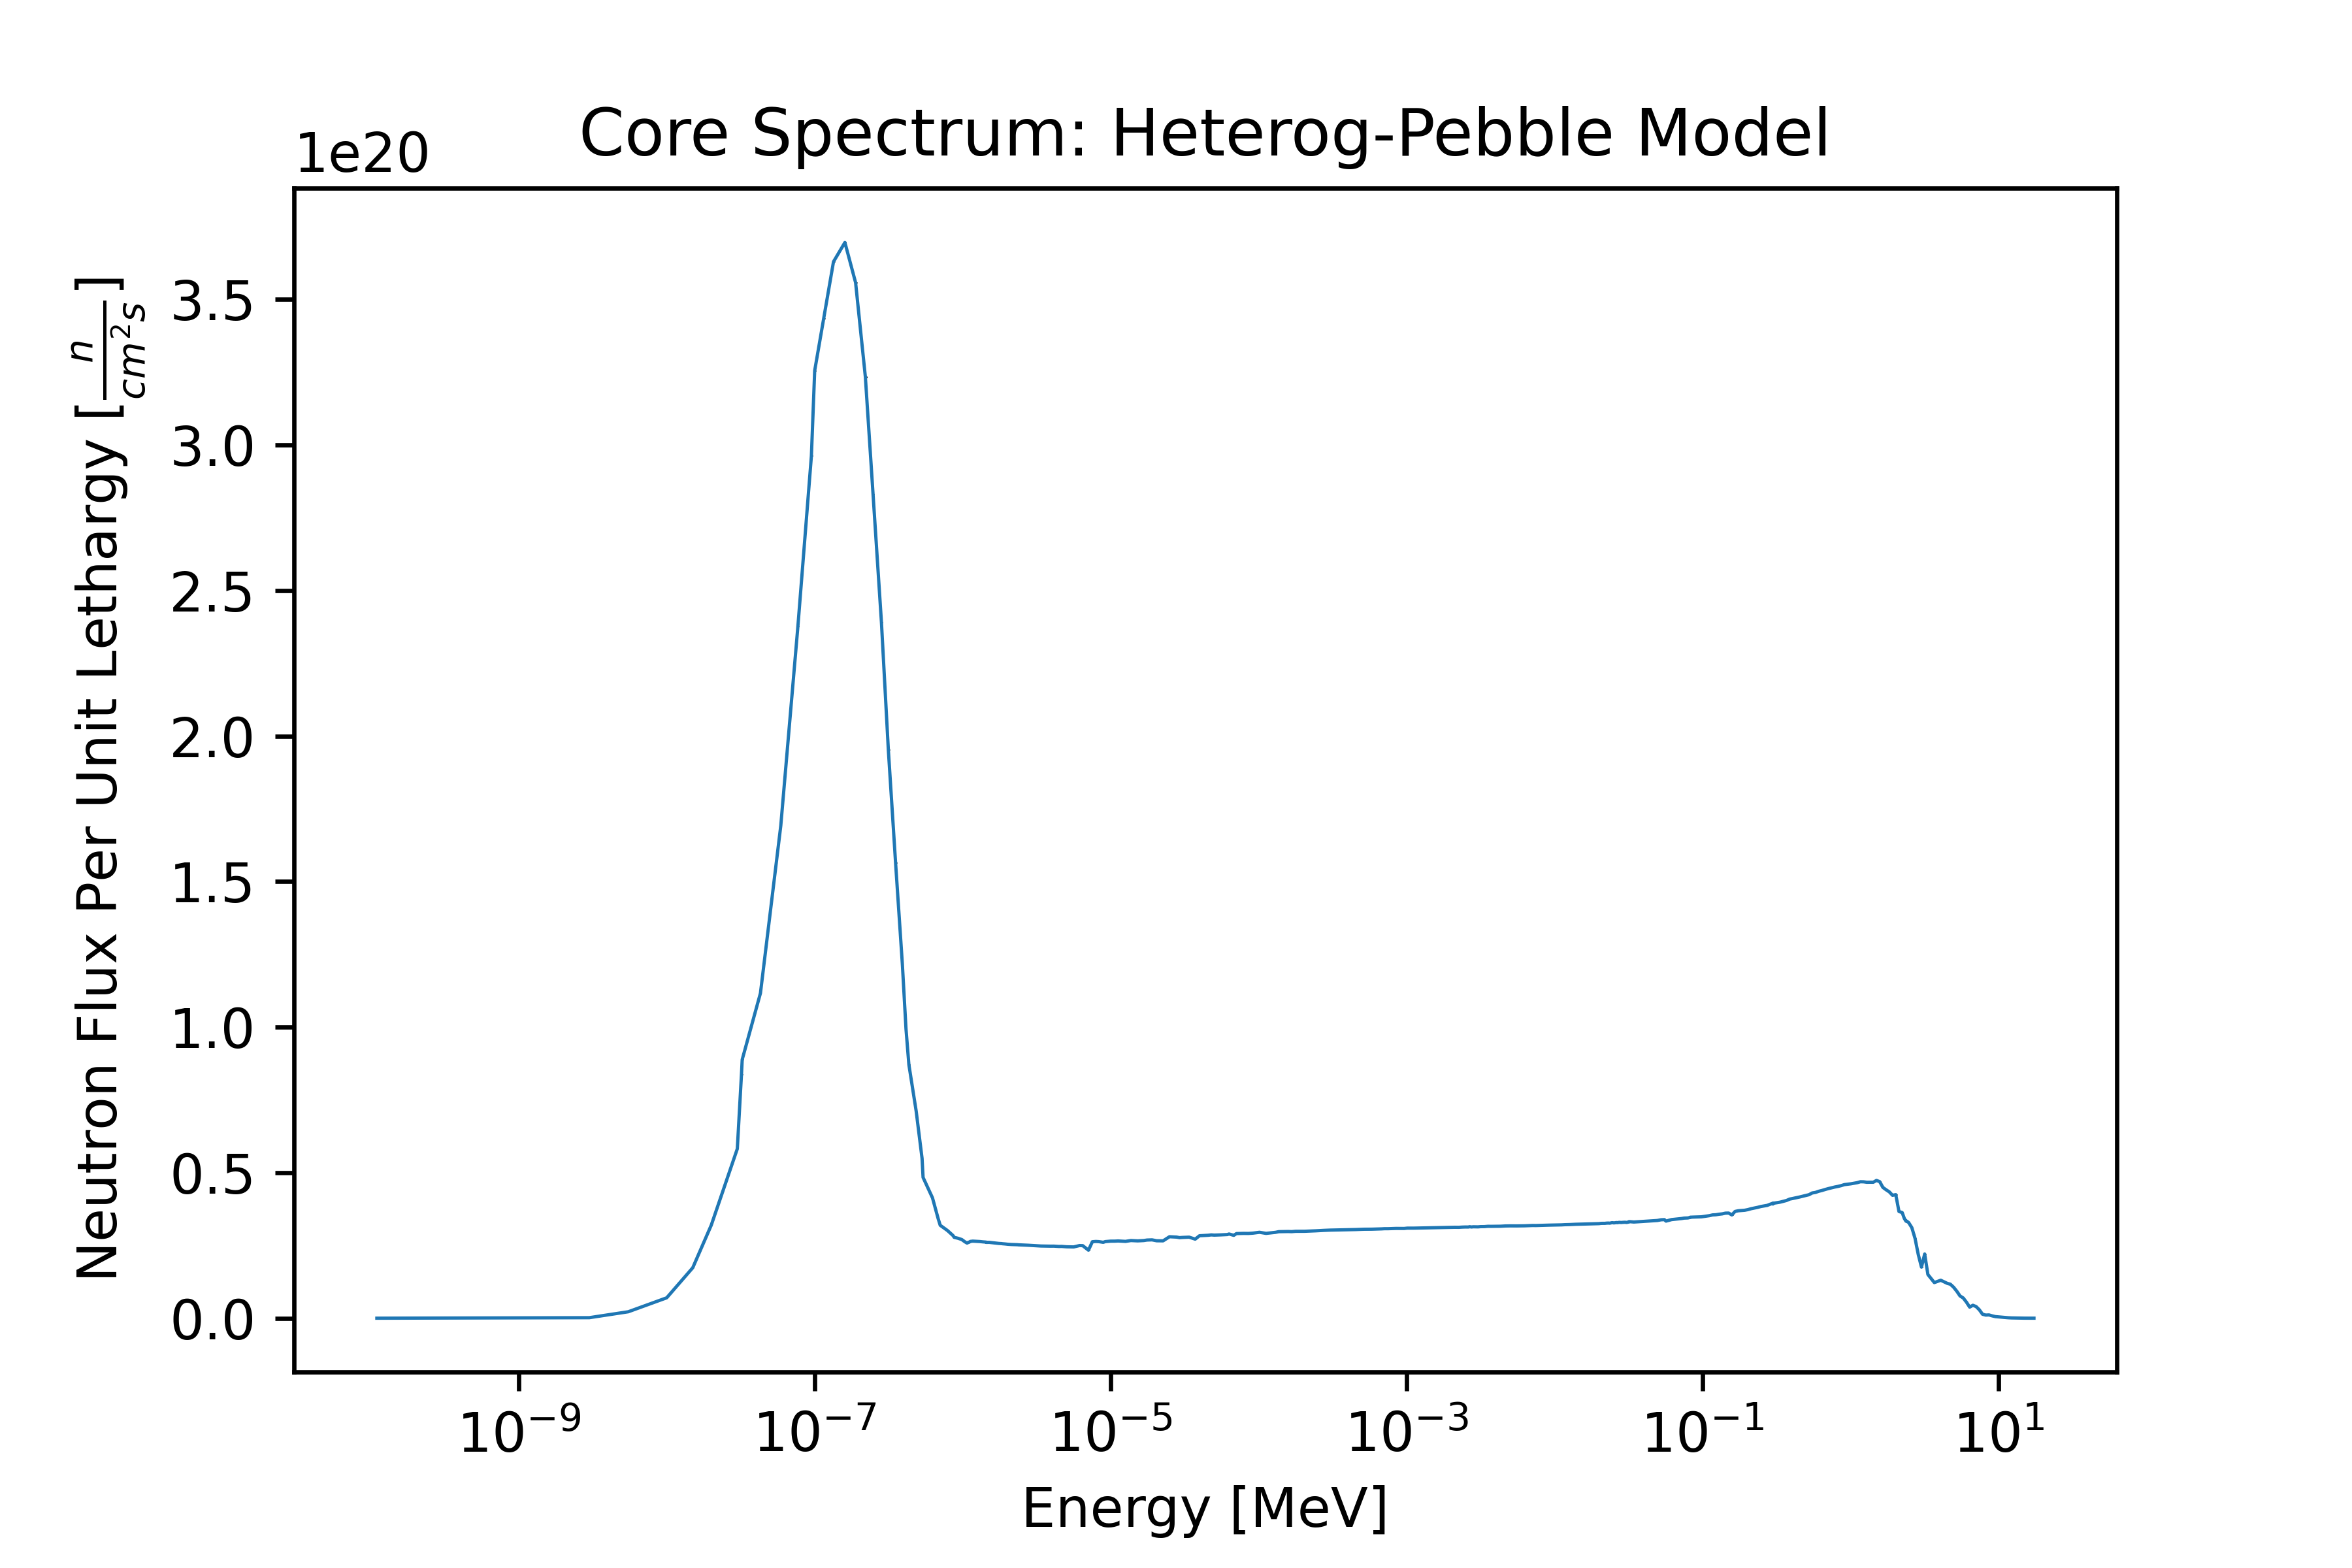
\includegraphics[width=0.95\linewidth]{figures/core_spec_het}
  \caption{Core Spectrum}
  \label{fig:het-core}
\end{subfigure}%

\caption{Lethargy Adjusted Neutron Flux Energy Spectra: Core Using Heterogenized Pebbles}
\end{figure}

\begin{figure}[H]\ContinuedFloat
\centering

\begin{subfigure}{0.95\textwidth}
  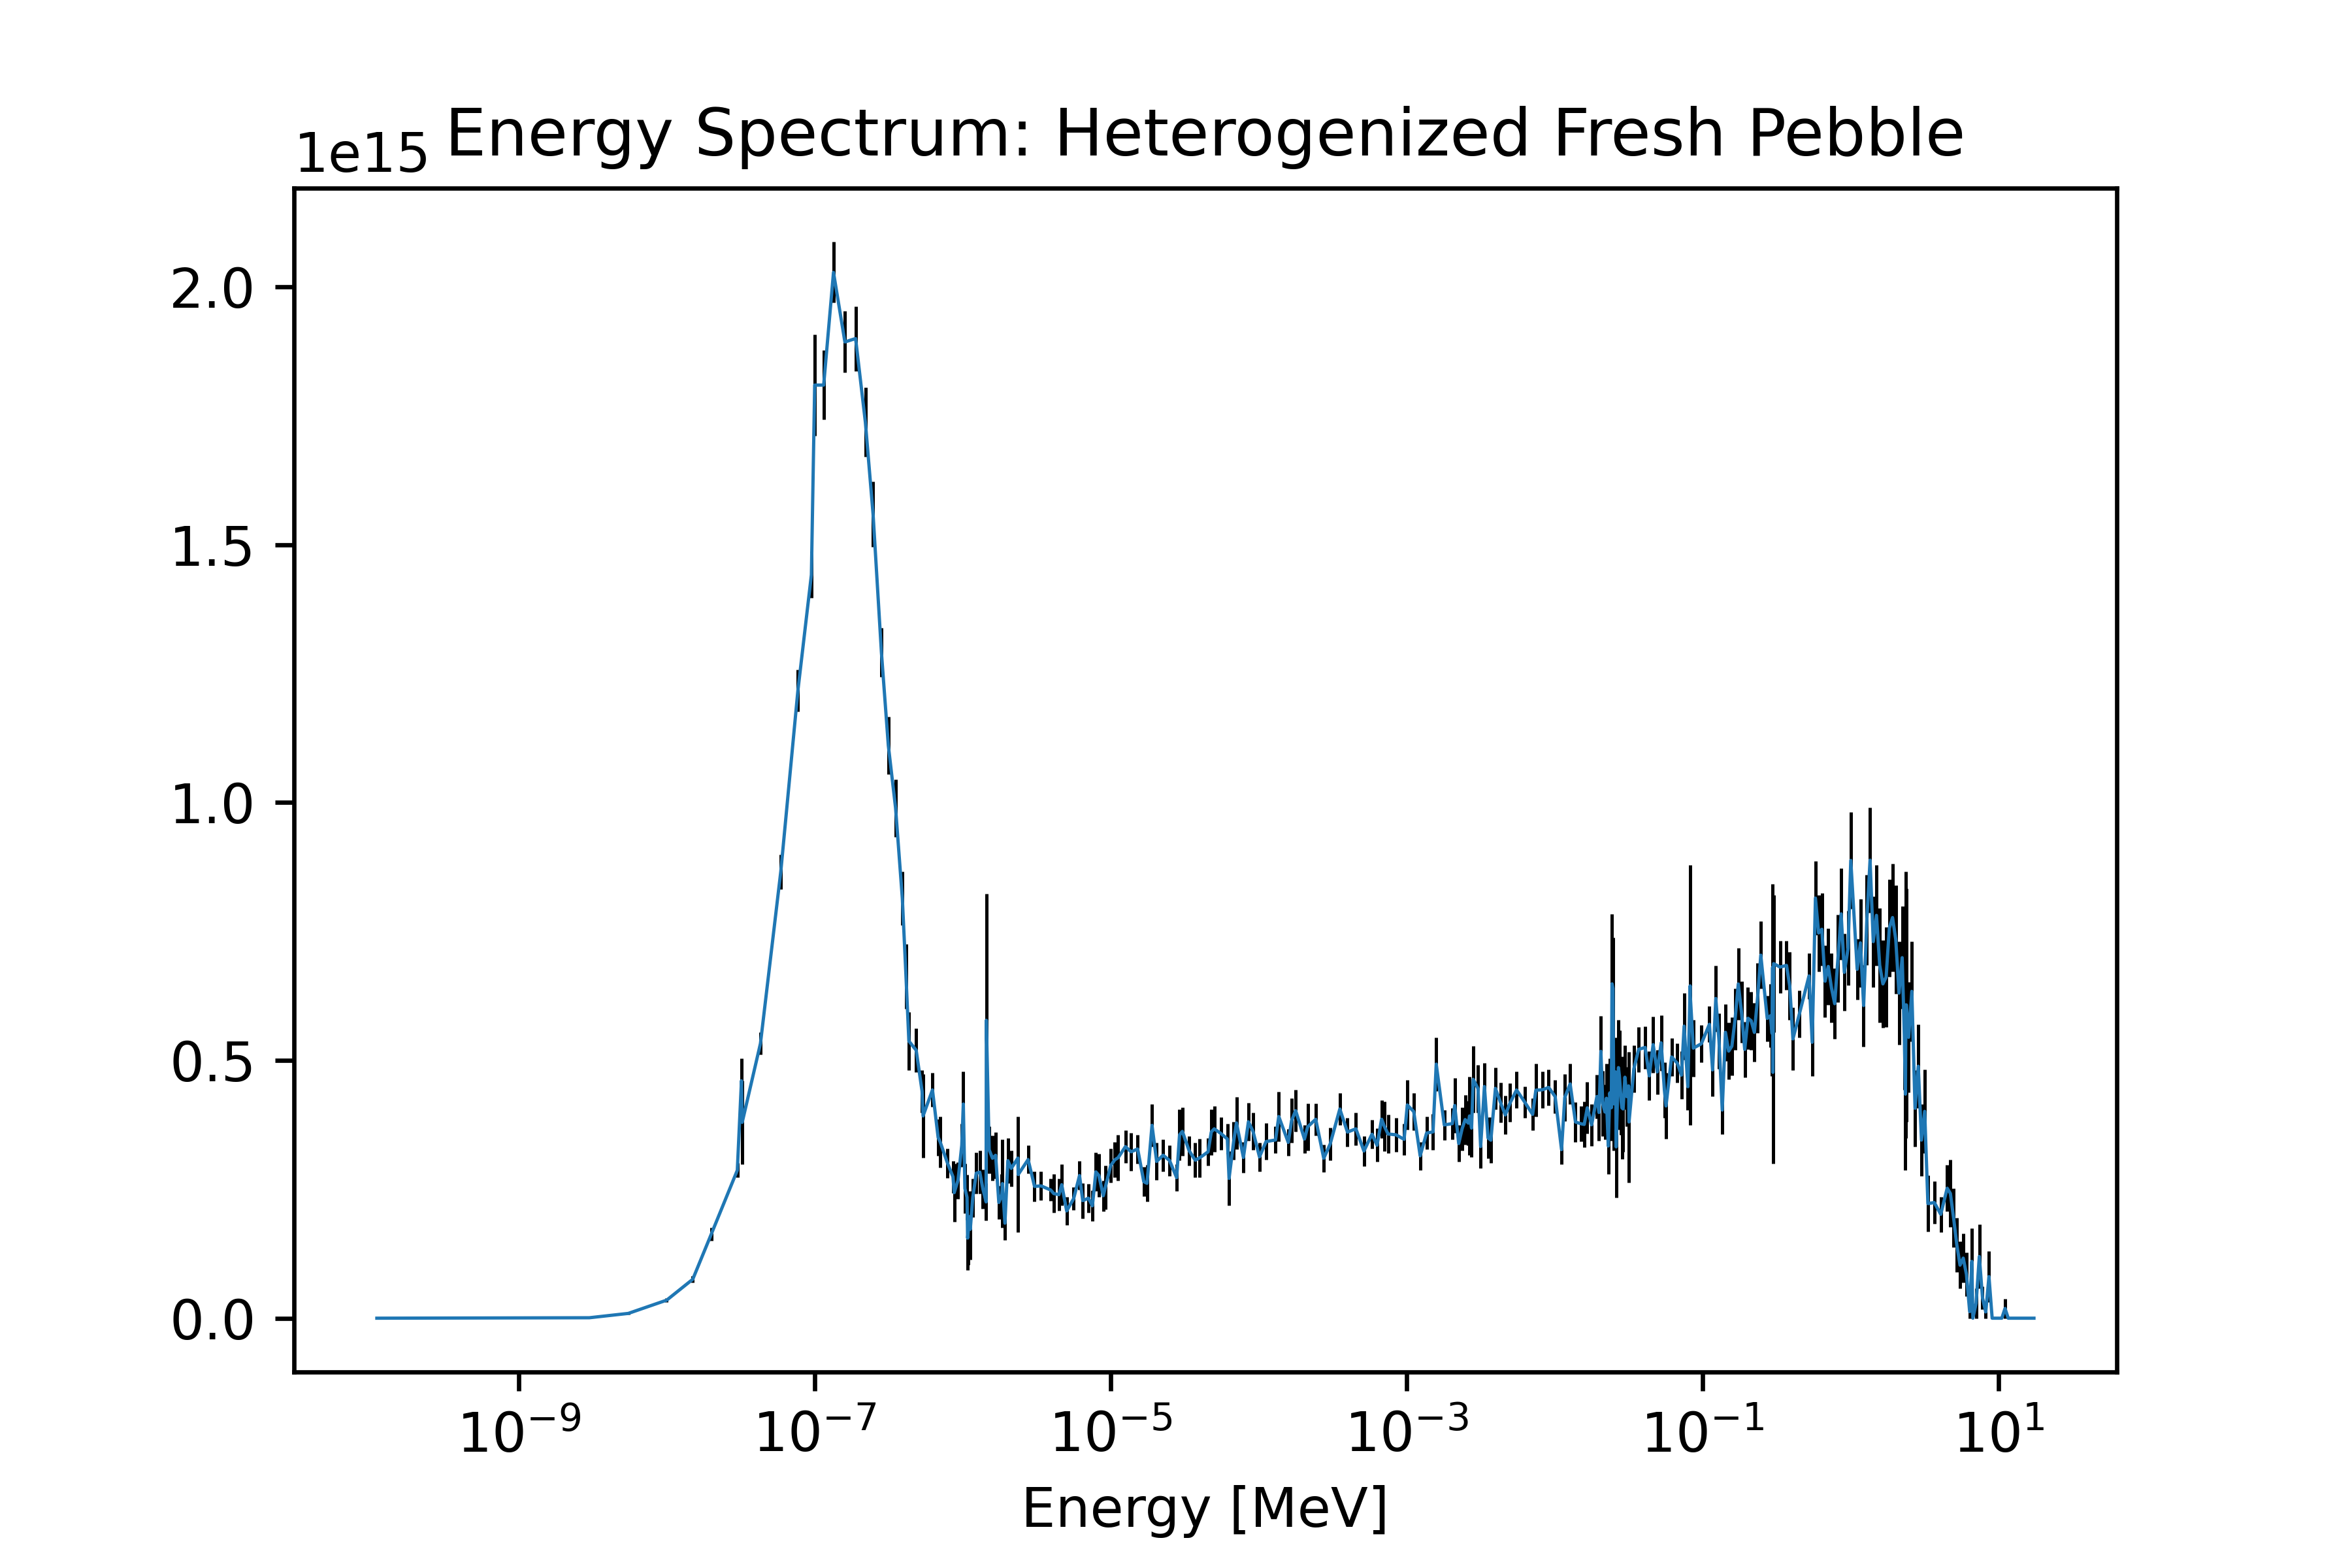
\includegraphics[width=0.95\linewidth]{figures/fresh_spec_het}
  \caption{Fresh Pebble Spectrum}
  \label{fig:het-fresh}
\end{subfigure}%


\begin{subfigure}{0.95\textwidth}
  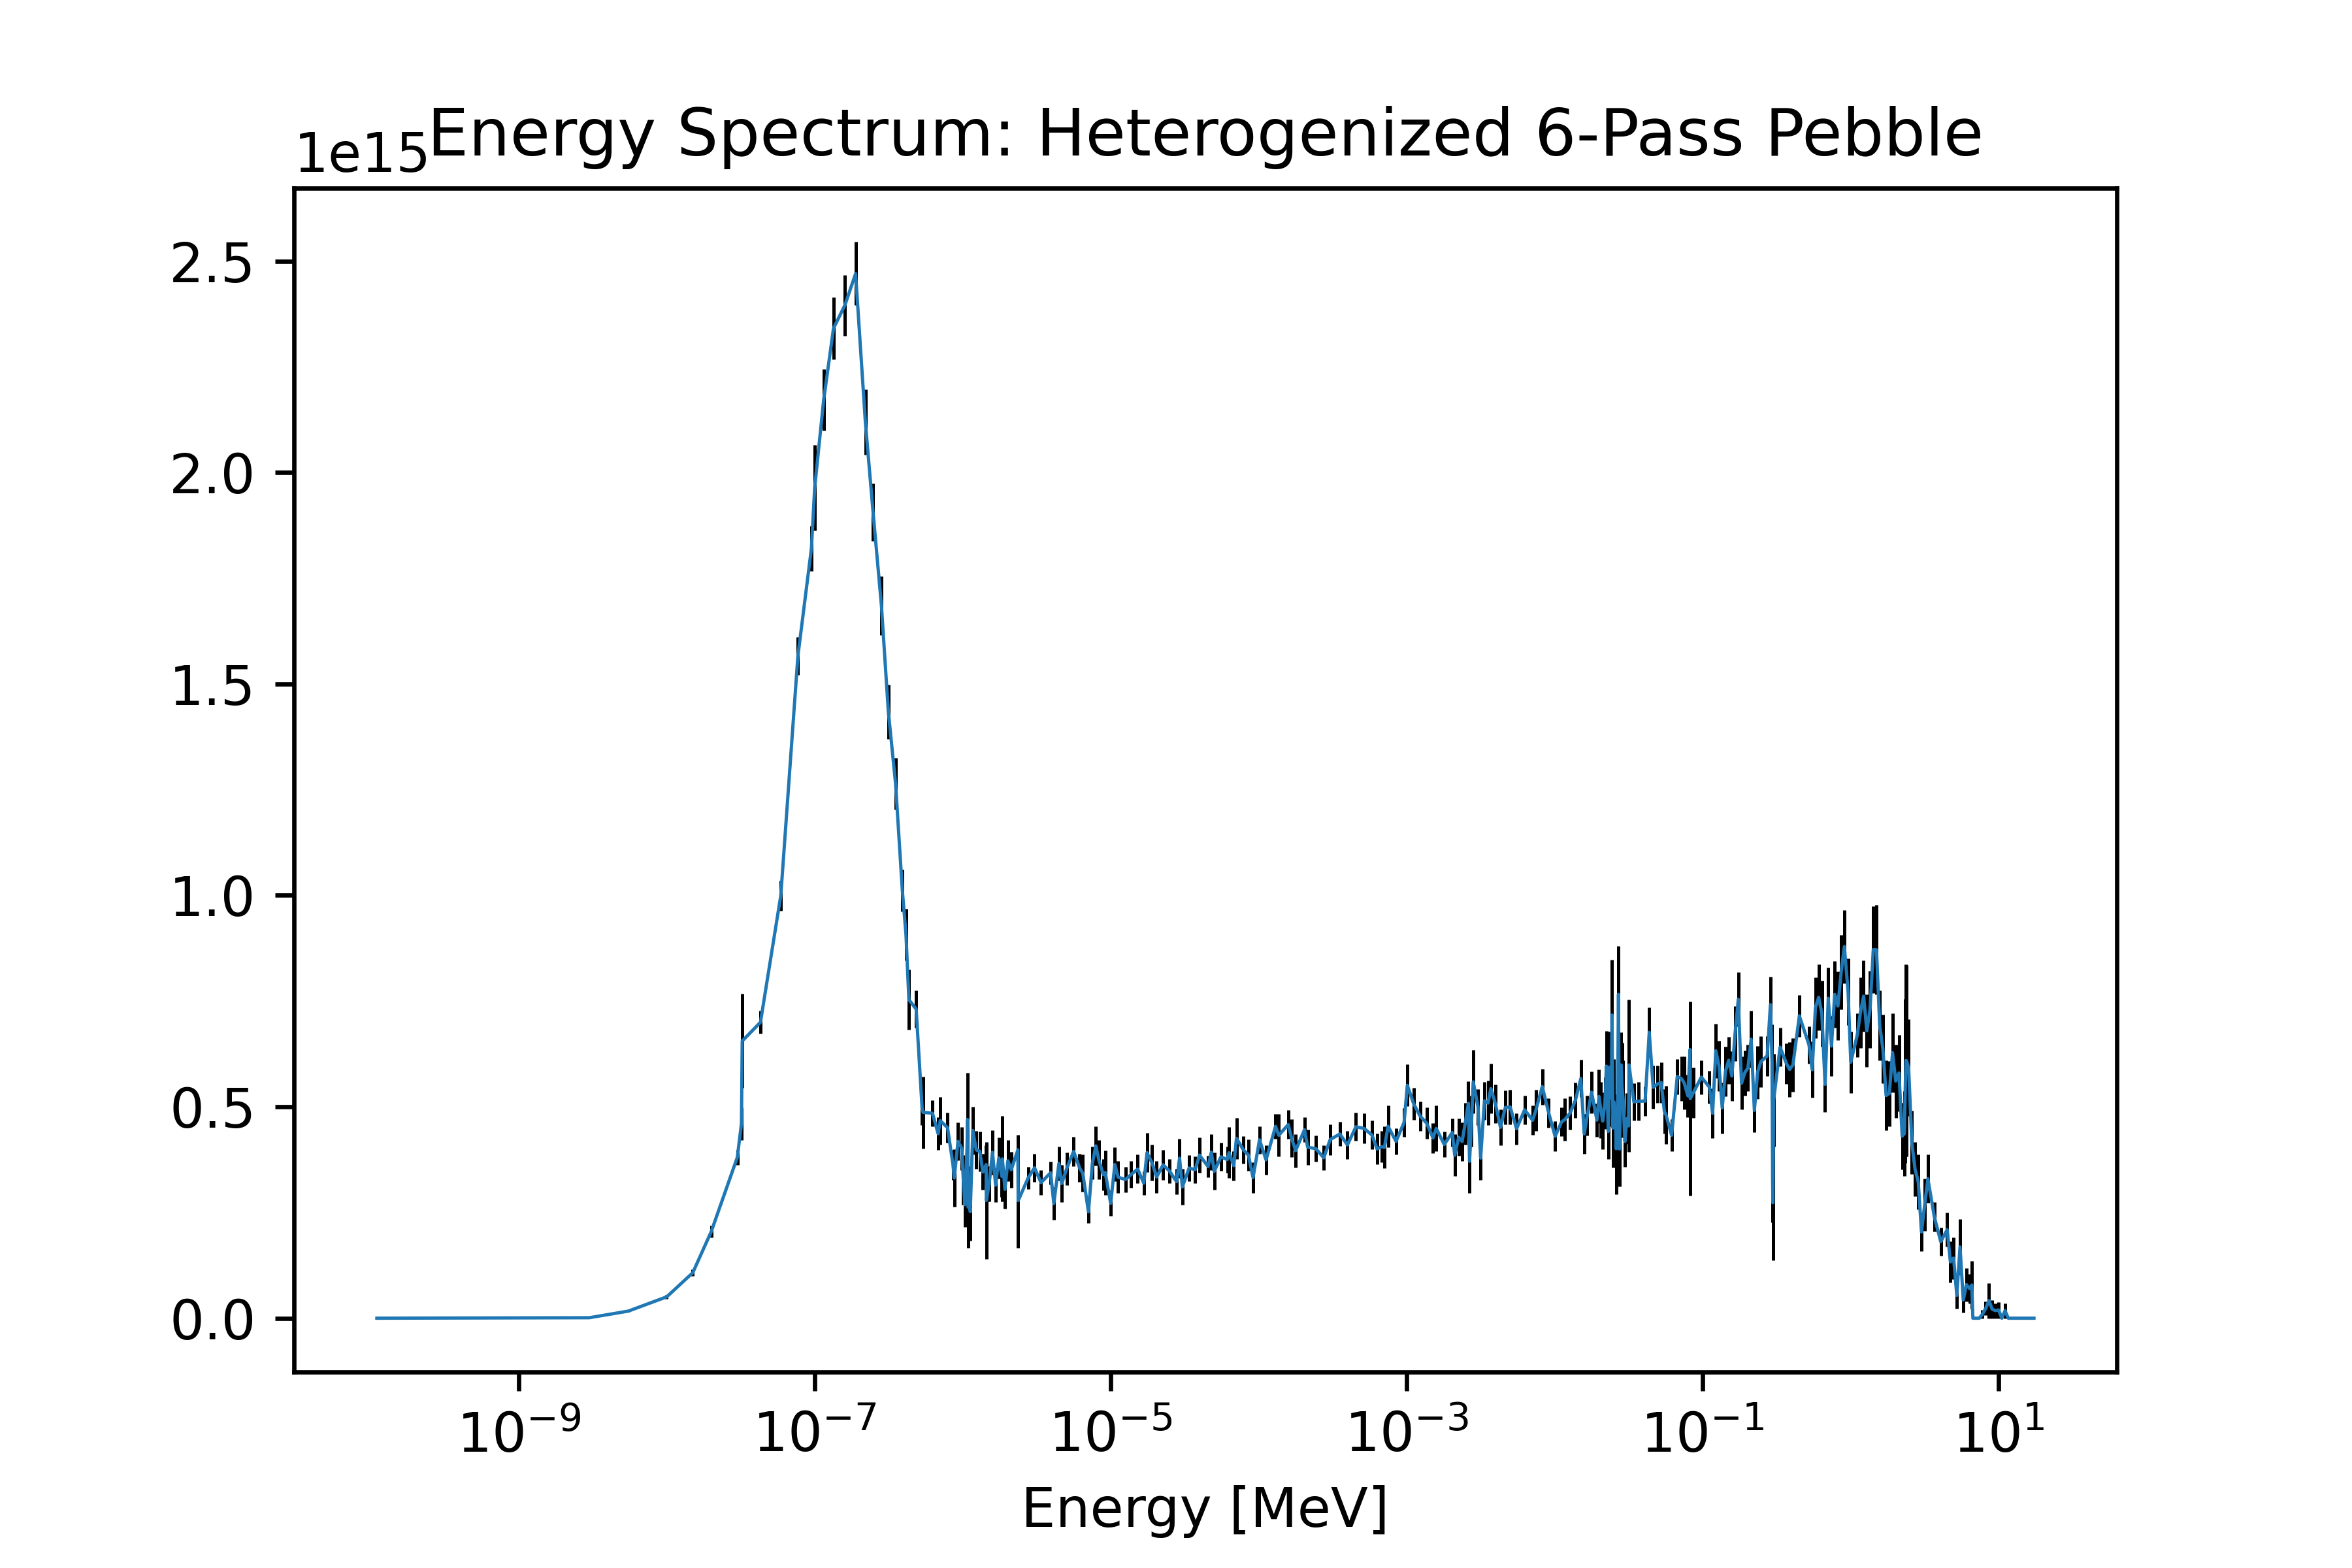
\includegraphics[width=0.95\linewidth]{figures/6_spec_het}
  \caption{Six-Pass Pebble Spectrum}
  \label{fig:het-six}
\end{subfigure}%

\caption{Lethargy Adjusted Neutron Flux Energy Spectra: Core Using Heterogenized Pebbles (cont.)}
\end{figure}

\begin{figure}[H]\ContinuedFloat
\centering

\begin{subfigure}{0.95\textwidth}
  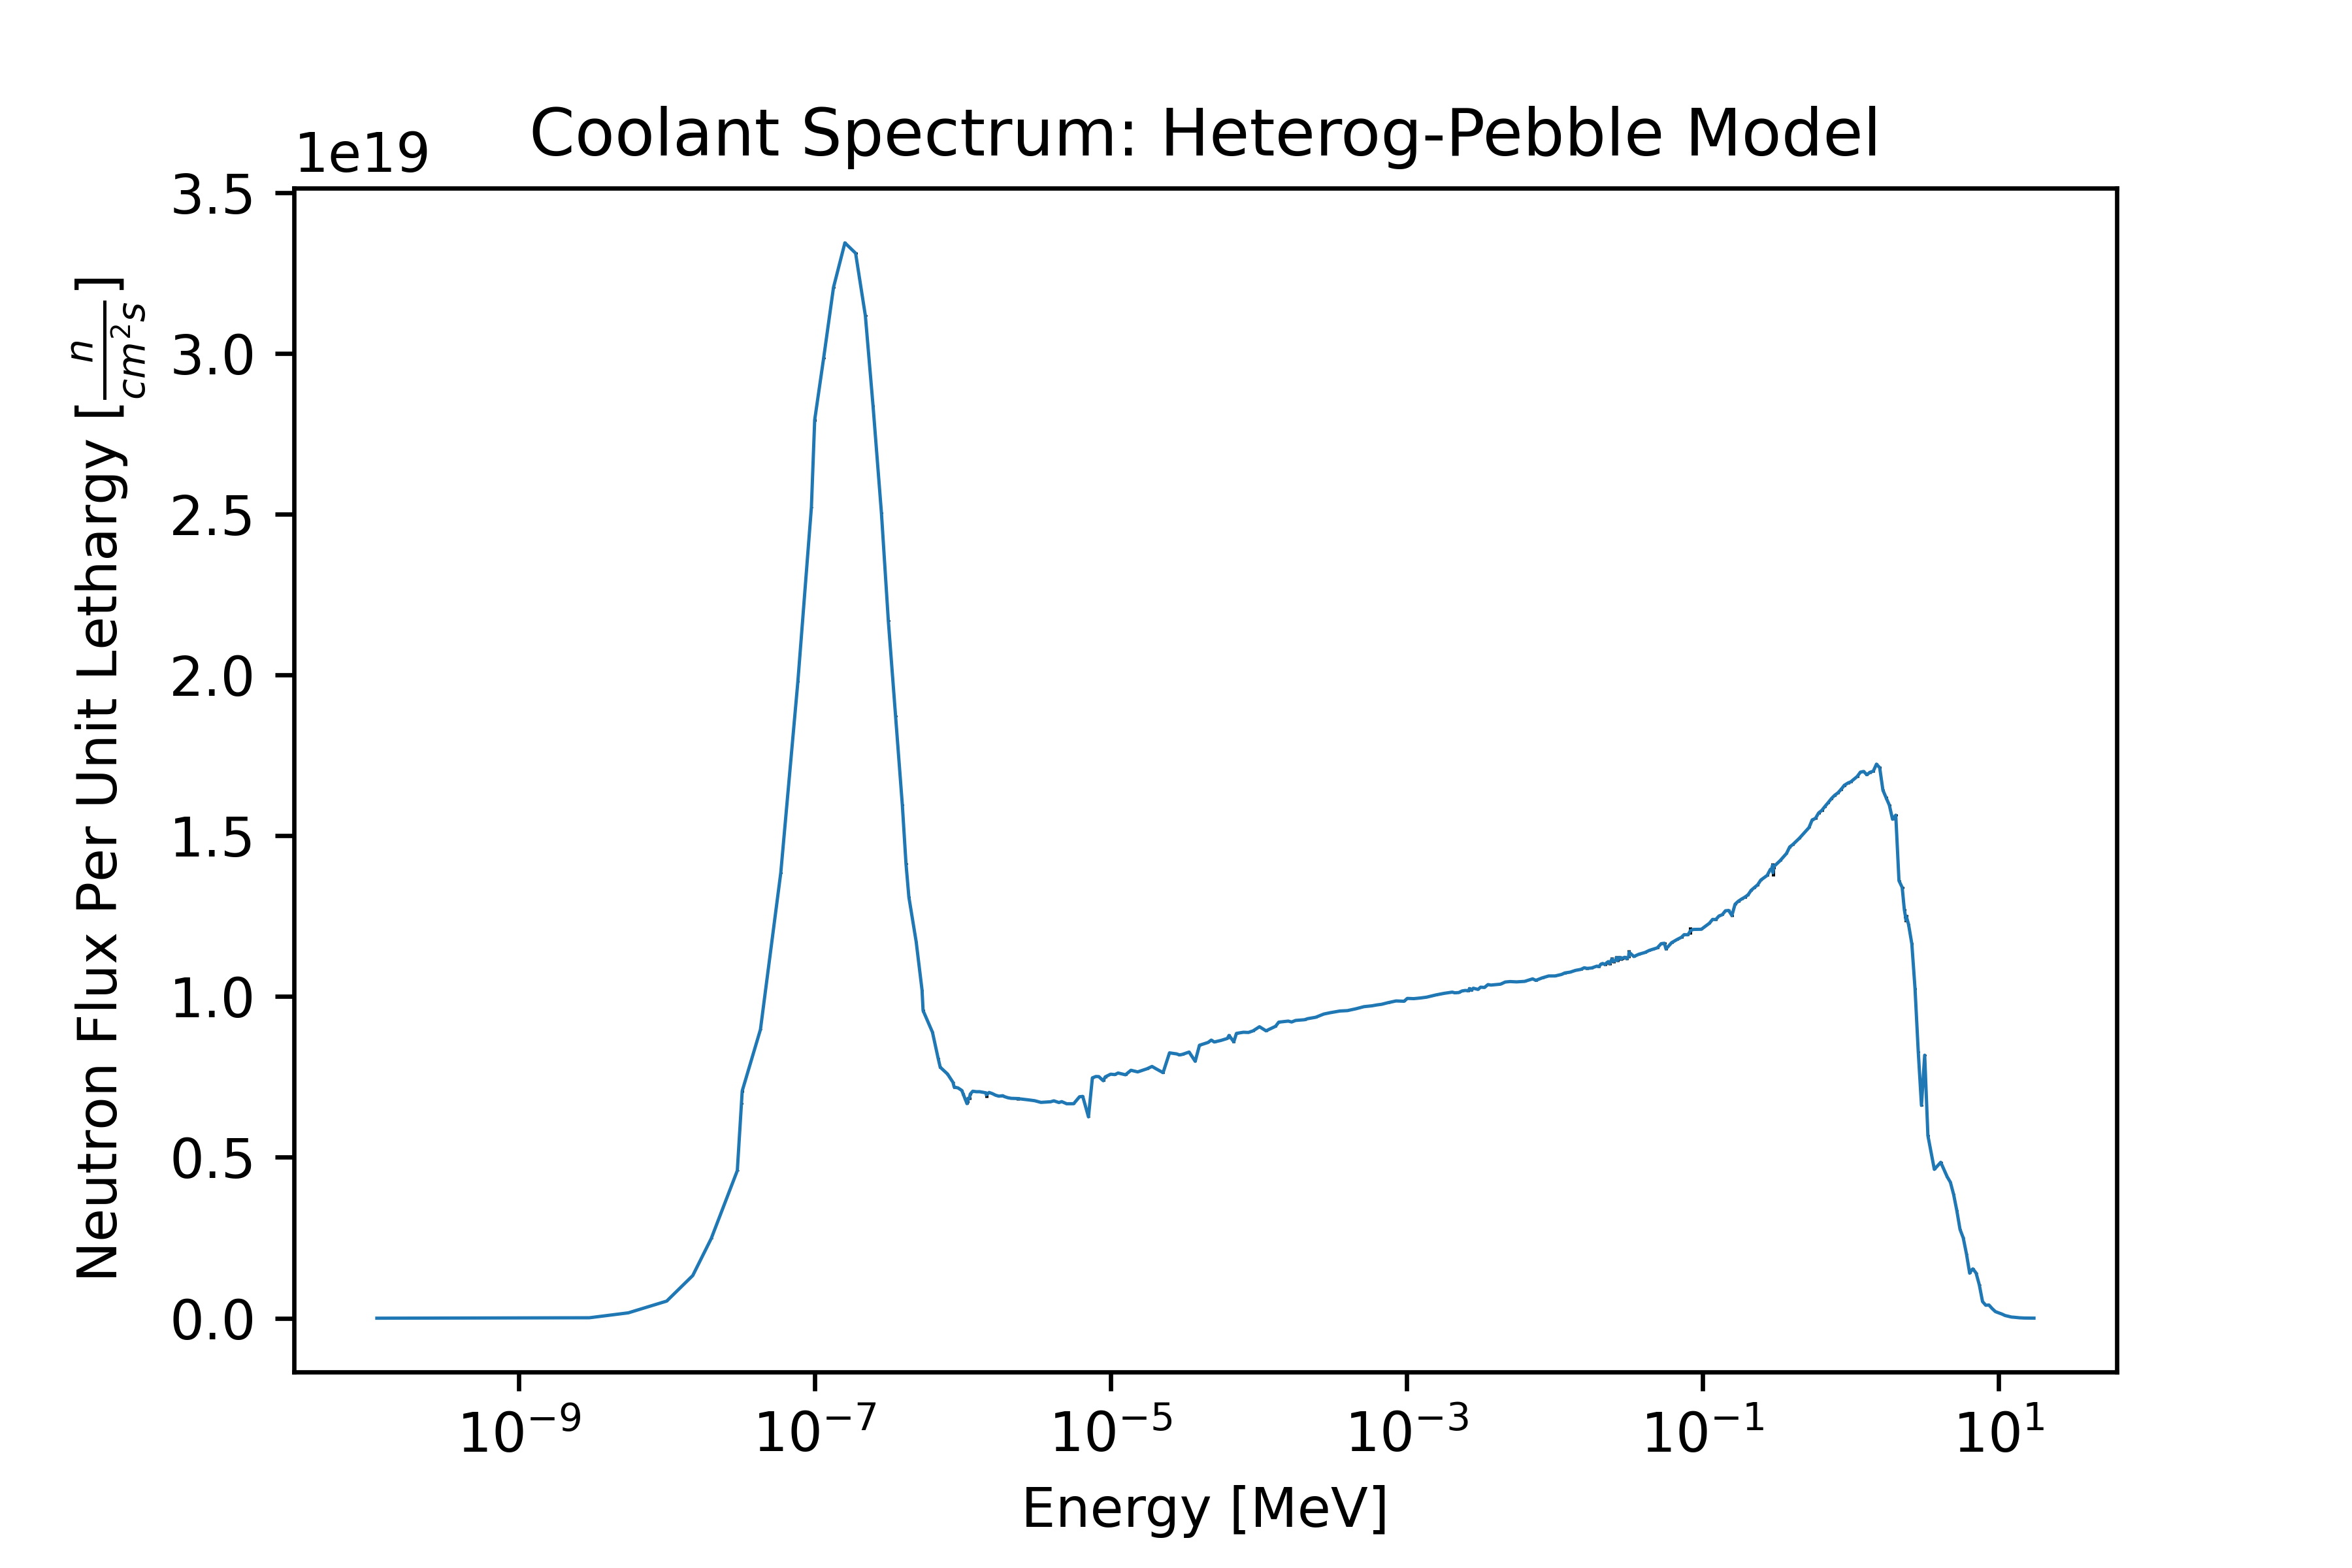
\includegraphics[width=0.95\linewidth]{figures/cool_spec_het}
  \caption{Coolant Spectrum}
  \label{fig:het-cool}
\end{subfigure}%


\begin{subfigure}{0.95\textwidth}
  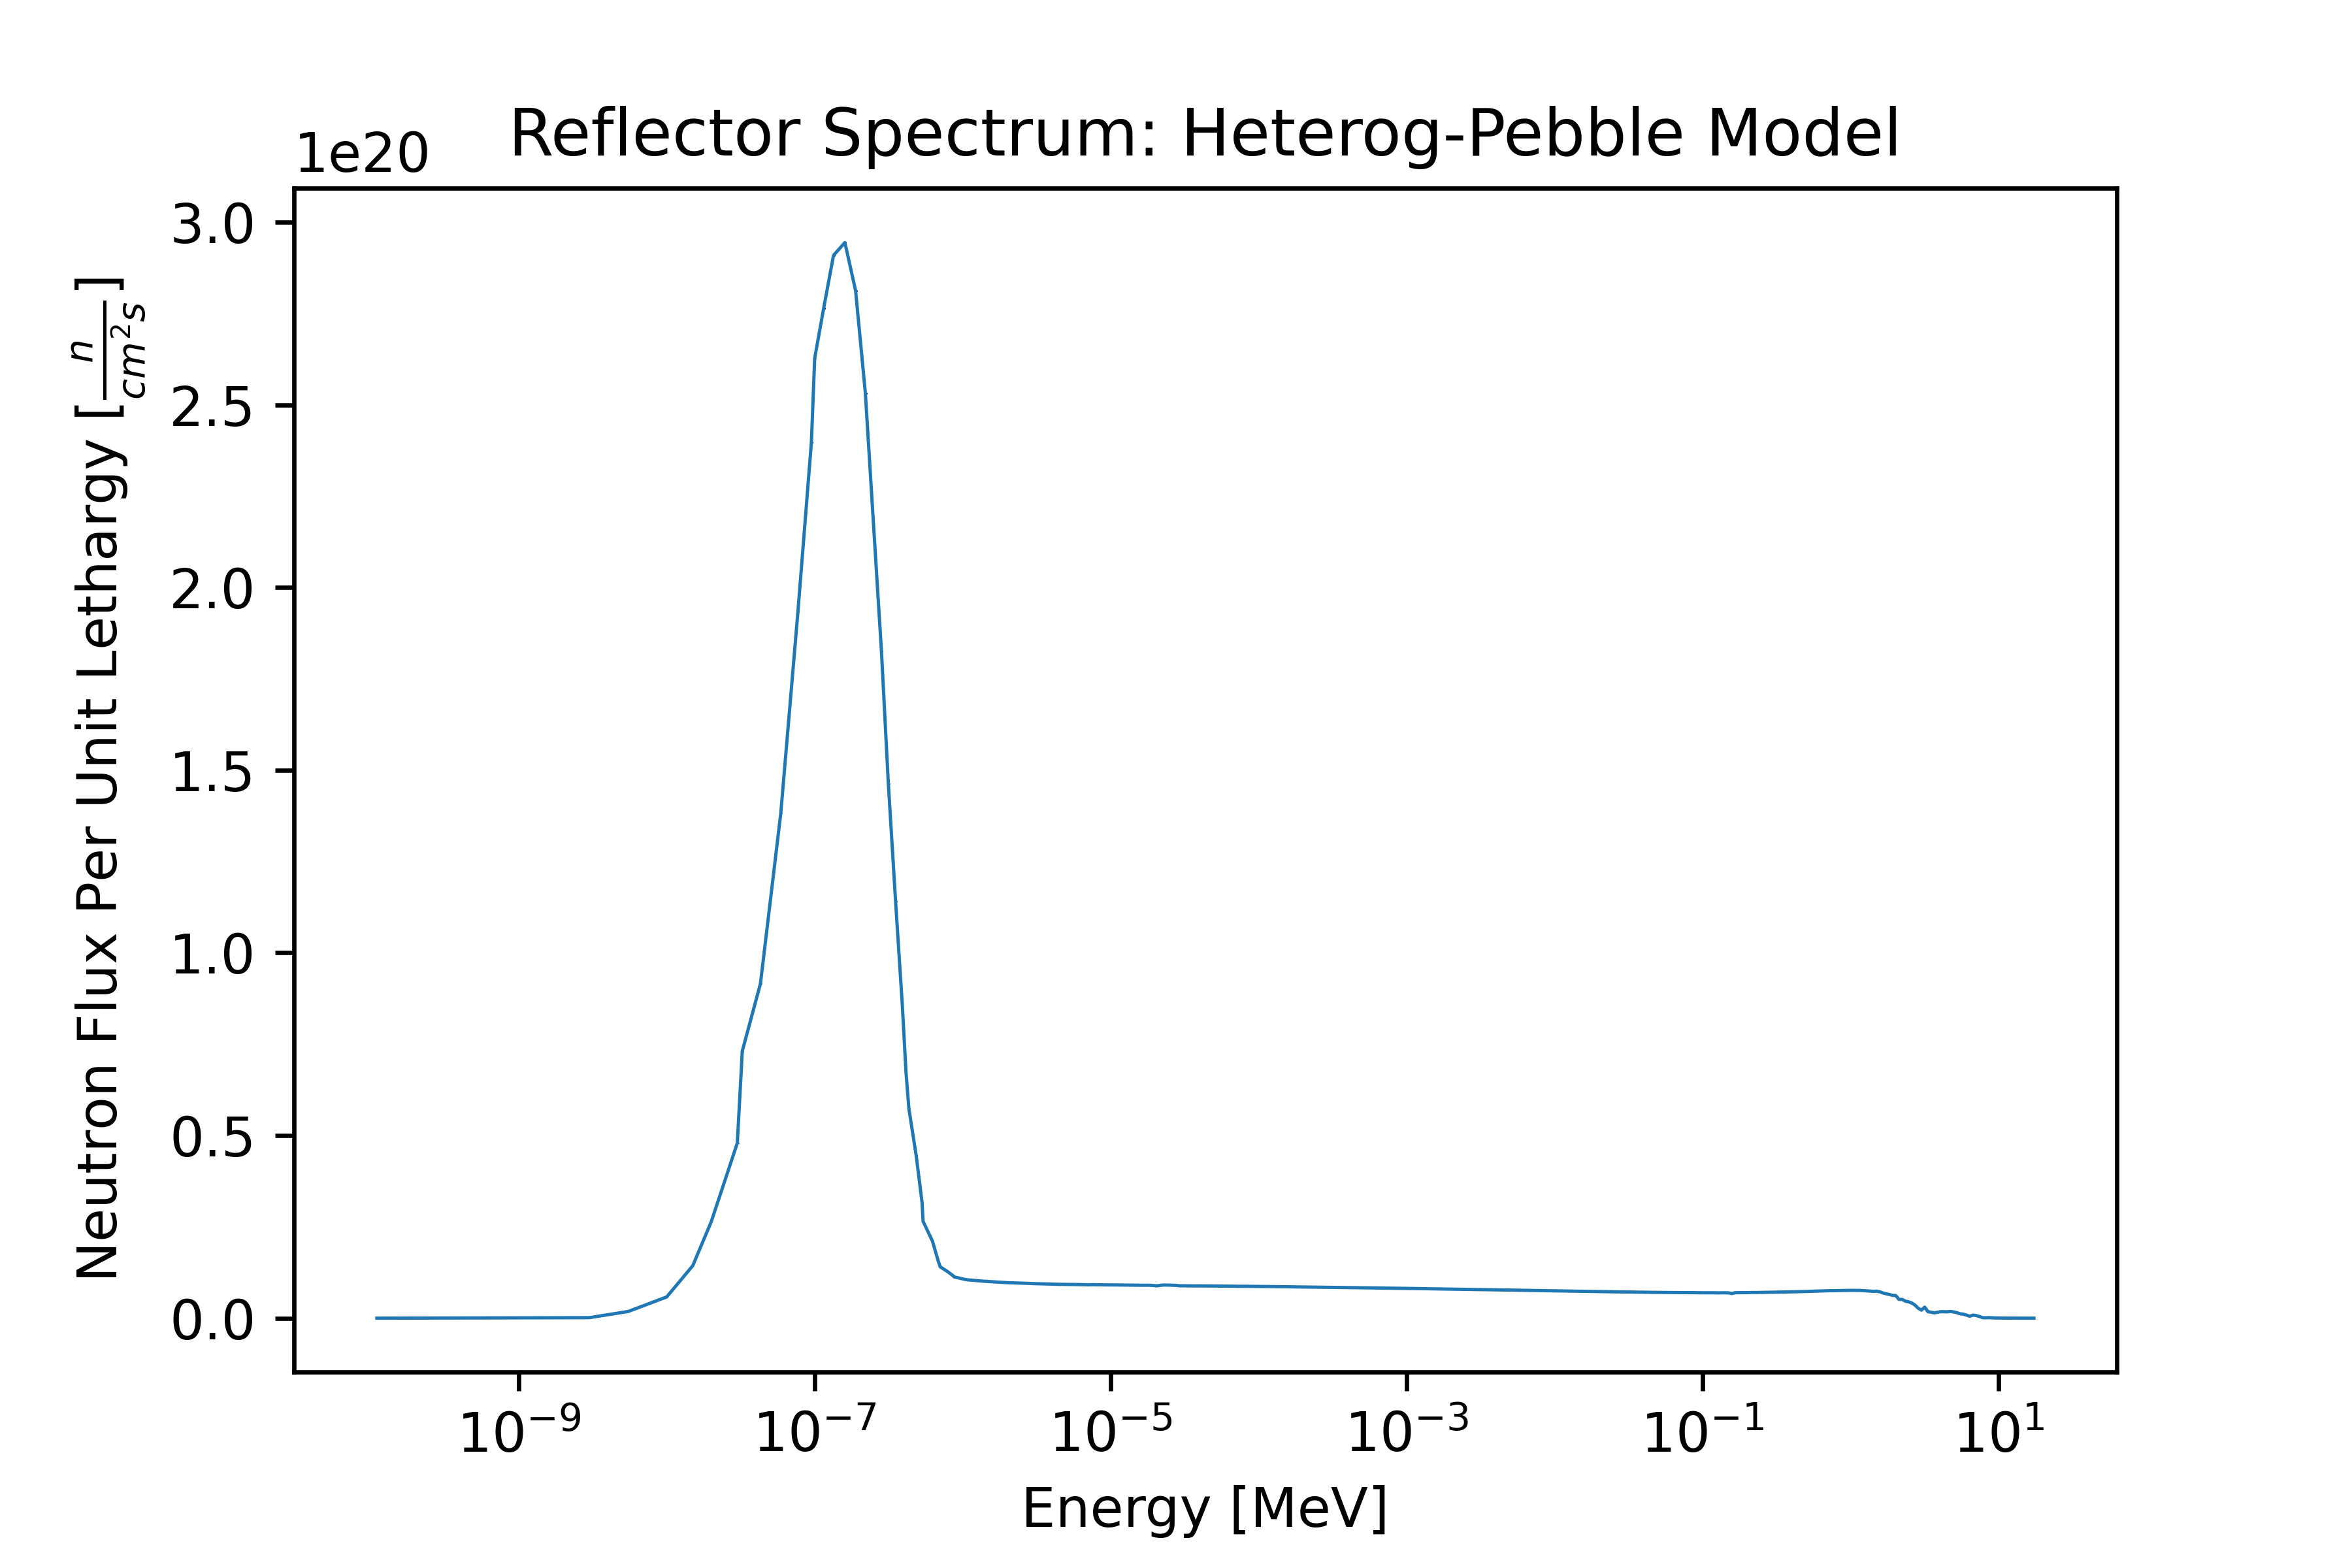
\includegraphics[width=0.95\linewidth]{figures/reflect_spec_het}
  \caption{Reflector Spectrum}
  \label{fig:het-reflec}
\end{subfigure}%


\caption{Lethargy Adjusted Neutron Flux Energy Spectra: Core Using Heterogenized Pebbles (cont.)}
\label{fig:hom-spec}
\end{figure}
\begin{figure}[H]
\centering
  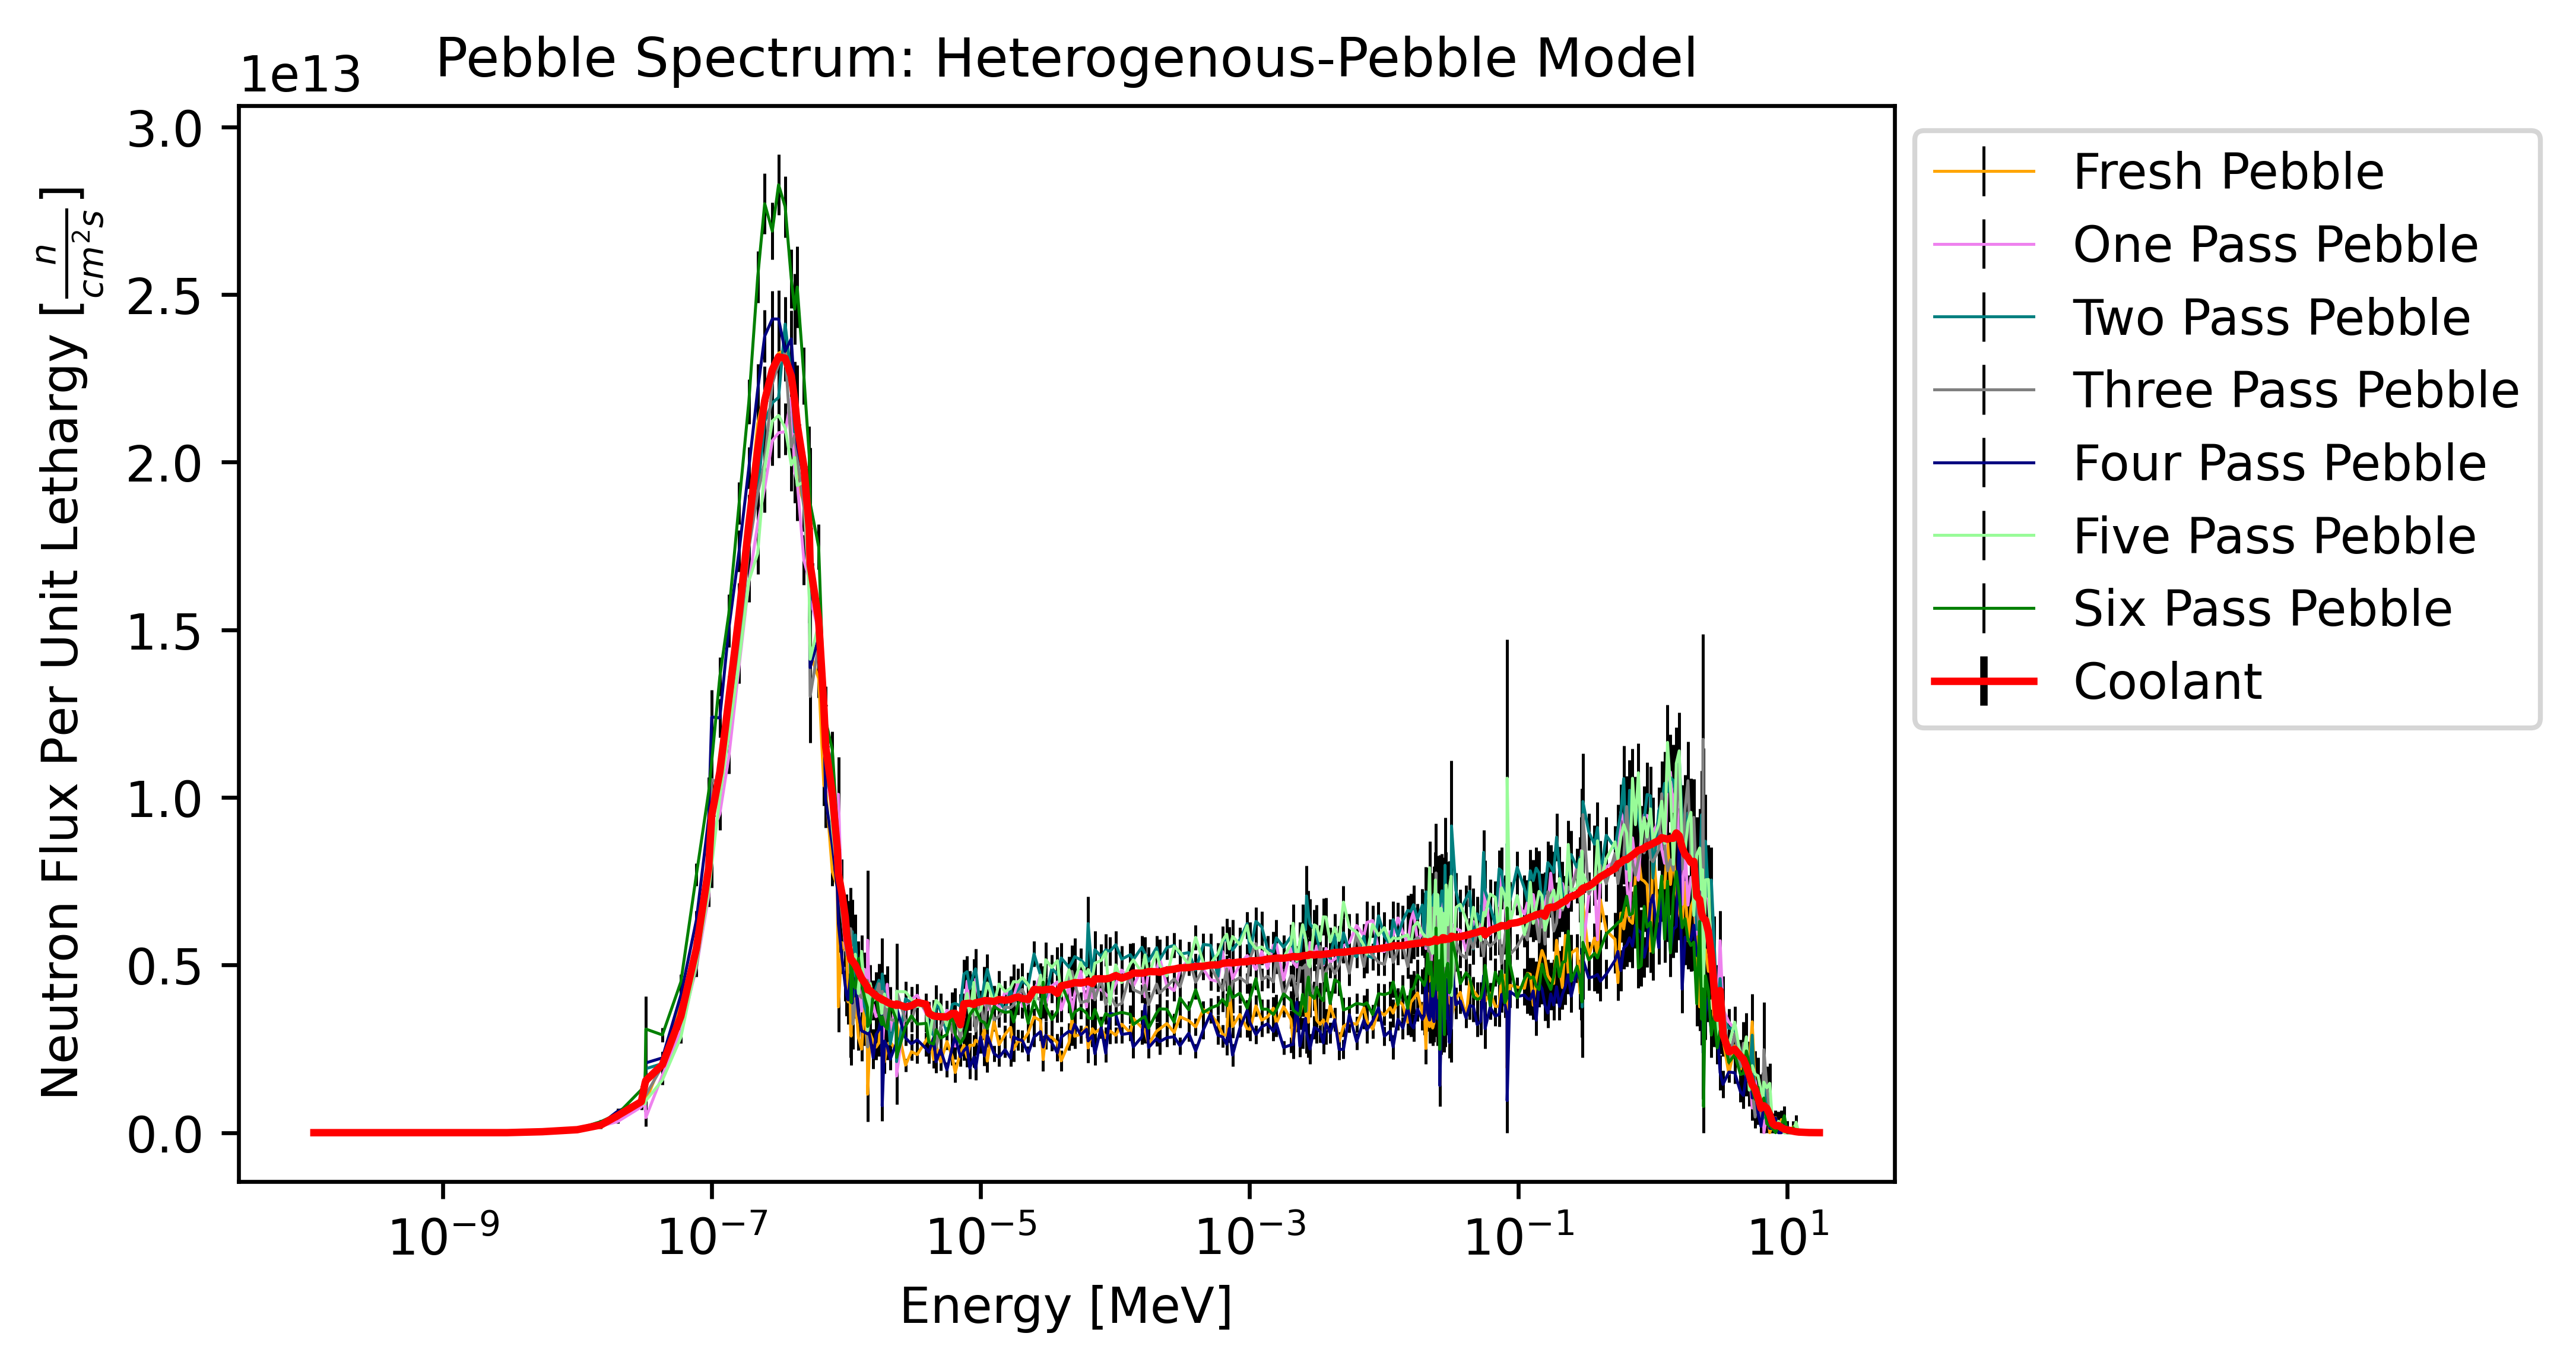
\includegraphics[width=0.95\linewidth]{figures/pebs_spec_het_er}
  \caption{Lethargy Adjusted Neutron Flux Energy Spectrum in the Each Pebble Burnup and Coolant for the Heterogenous-Pebble Sangamon20}
  \label{fig:het-peb}
\end{figure}


The spectra for the Sangamon20 core using heterogenized TRISO particles are shown in Figure \ref{fig:het-all}.  Much like the flux profiles in \ref{fig:het-det-xy} and \ref{fig:het-det-z}, the heterogeneous model's spectra are of a similar morphology to the homogenized spectra.  Figure \ref{fig:het-peb} shows the pebble spectra for the heterogeneous pebble model, and, much like the combined pebble and coolant spectra in \ref{fig:hom-peb}, the coolant spectrum roughly follows the average of the pebble spectra.

In order to better examine the differences between the homogenized and heterogenized versions, Figures \ref{fig:diff-flux} and \ref{fig:diff-spec} plot the simple relative difference for all spectra, and the radial fast and thermal profiles.  The relative difference calculation used the following:

\begin{align}
\Delta i &= \frac{i_{hom} - i_{het}}{i_{het}}
\intertext{where}
\Delta i&= \mbox{ relative difference for parameter i between homogenized and heterogenized model }\nonumber\\
i_{hom}&= \mbox{ homogenized parameter i}\nonumber\\
i_{het}&= \mbox{ heterogenized parameter i}\nonumber\\
\end{align}

And error calculation followed error propagation rules as shown in  \cite{taylor_chapter_1997}.


\begin{figure}[H]
\centering

\begin{subfigure}{0.9\textwidth}
  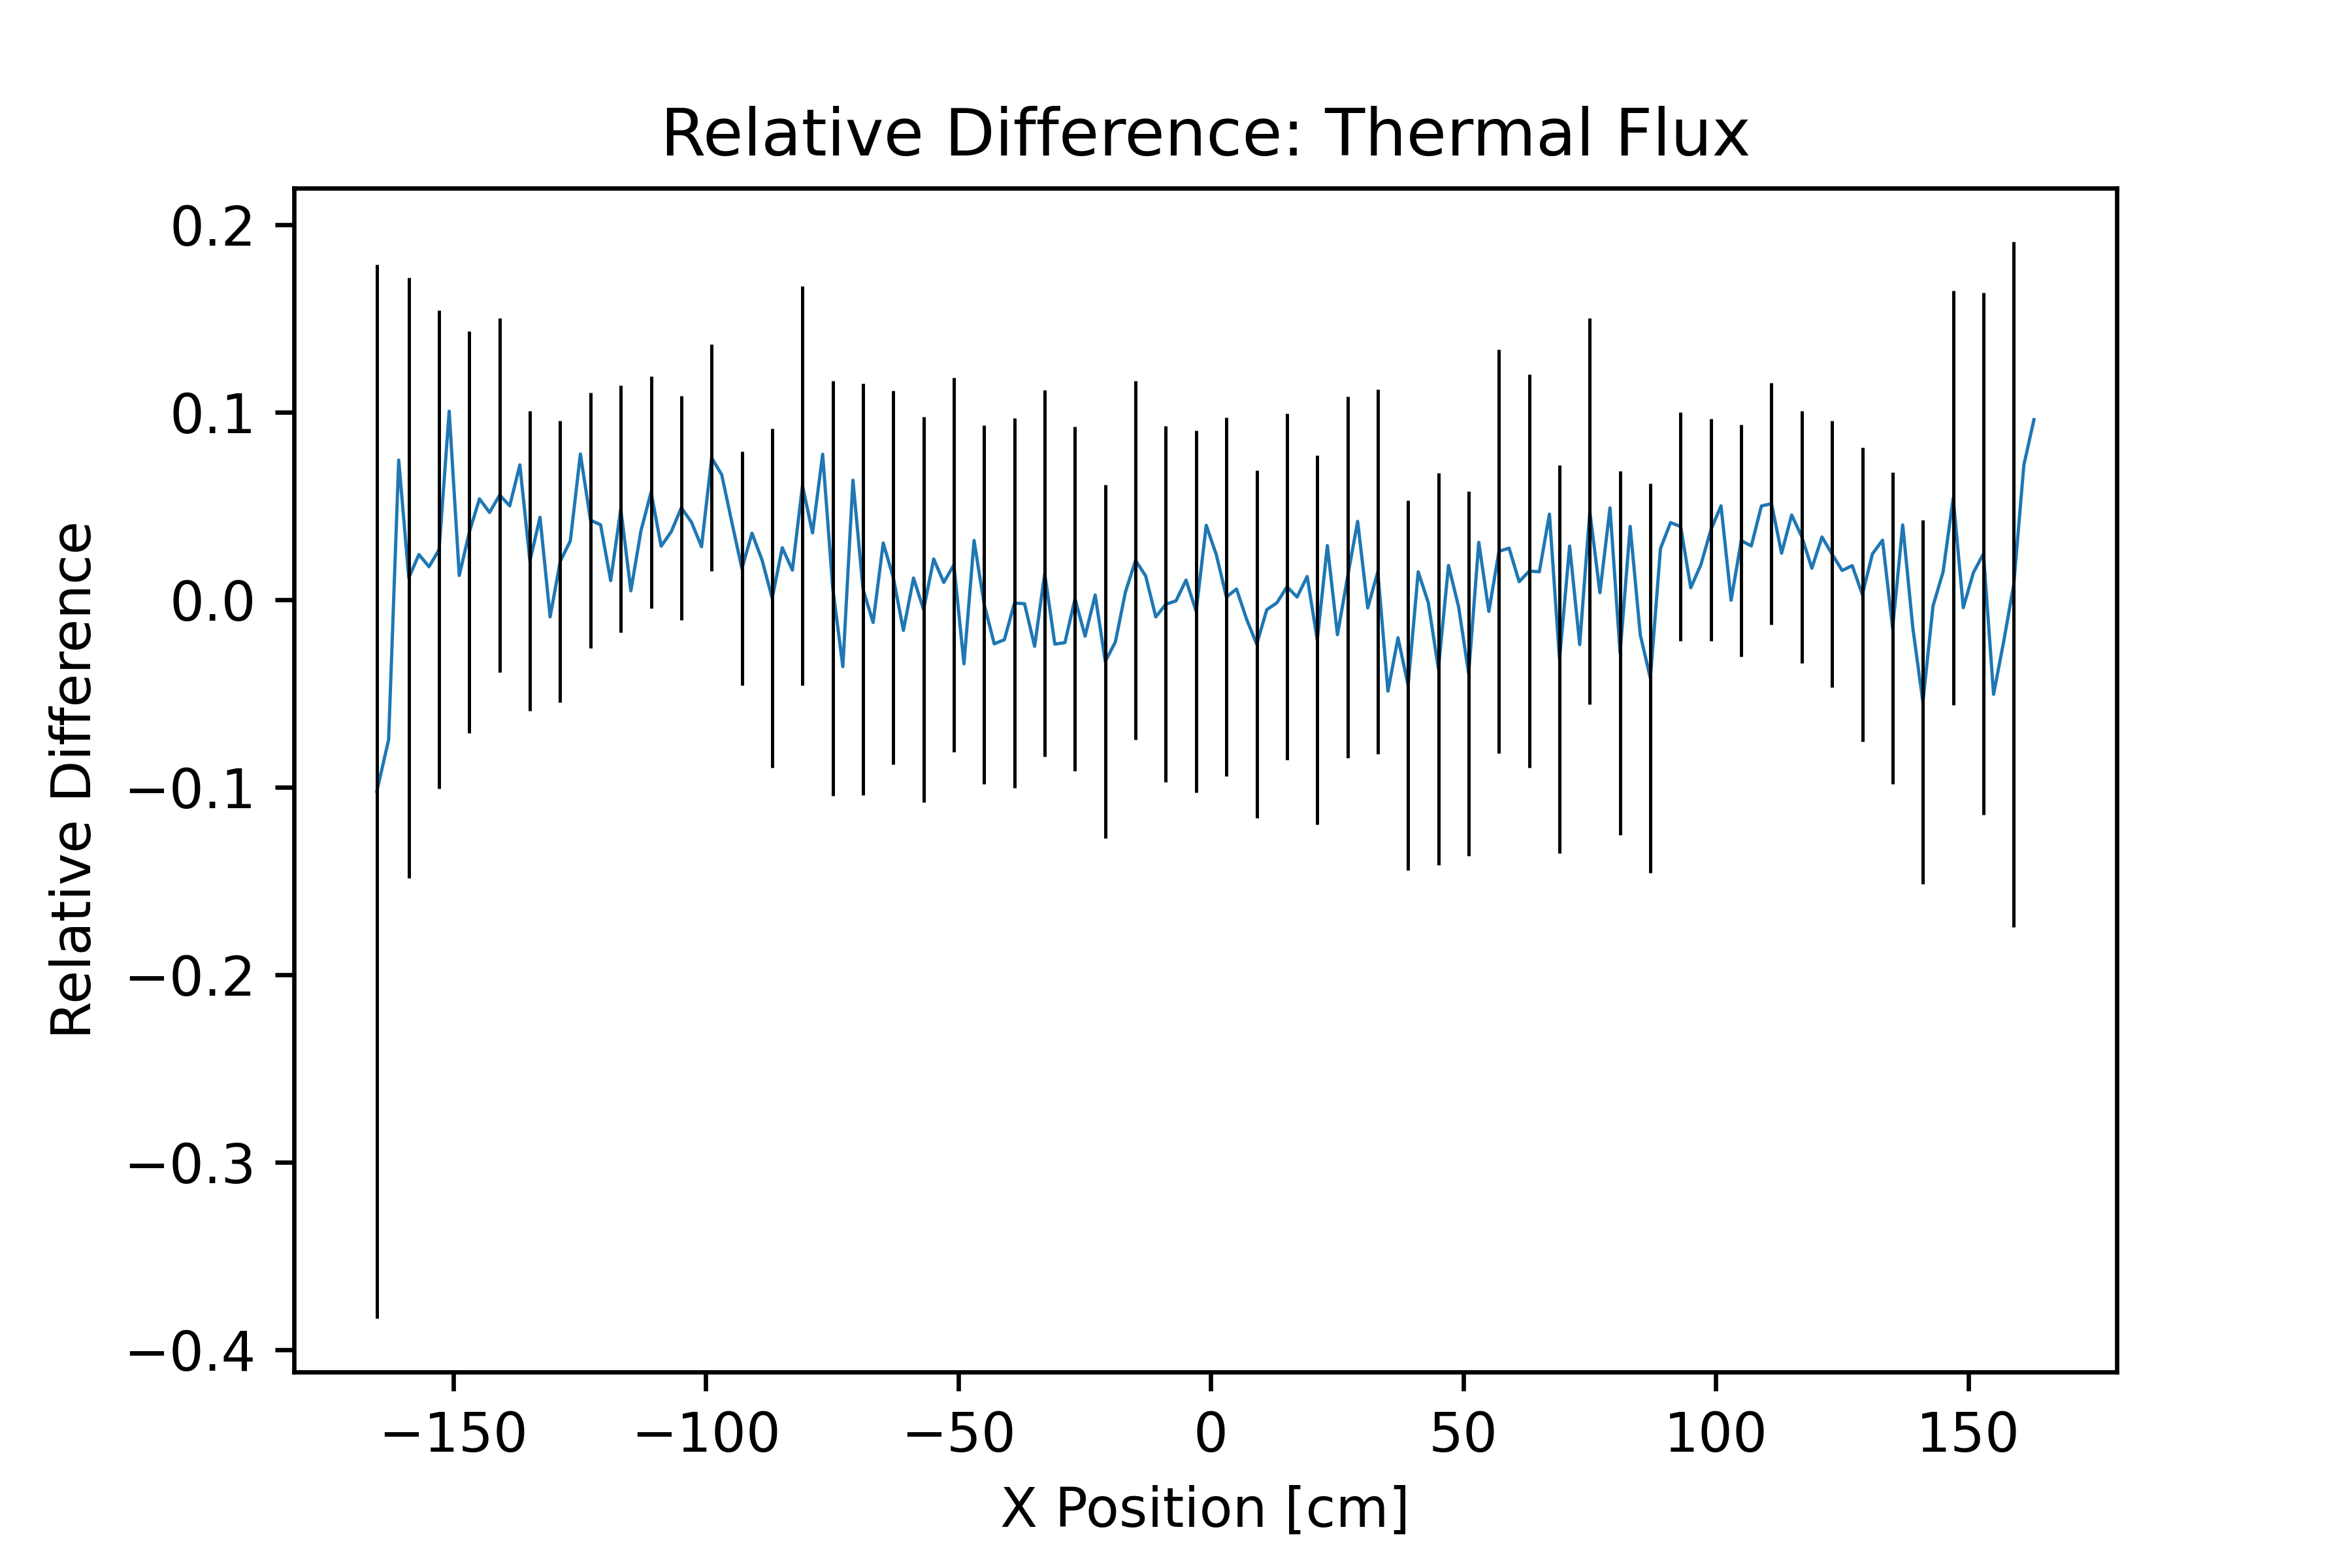
\includegraphics[width=0.9\linewidth]{figures/reldiff_therm_flux.png}
  \caption{Thermal Flux}
  \label{fig:diff-therm}
\end{subfigure}%

\caption{Relative Difference in Radial Thermal and Fast Flux Profiles Between Cores Using Homogenized and Heterogenized Pebbles}
\end{figure}

\begin{figure}[H]\ContinuedFloat
\centering

\begin{subfigure}{0.9\textwidth}
  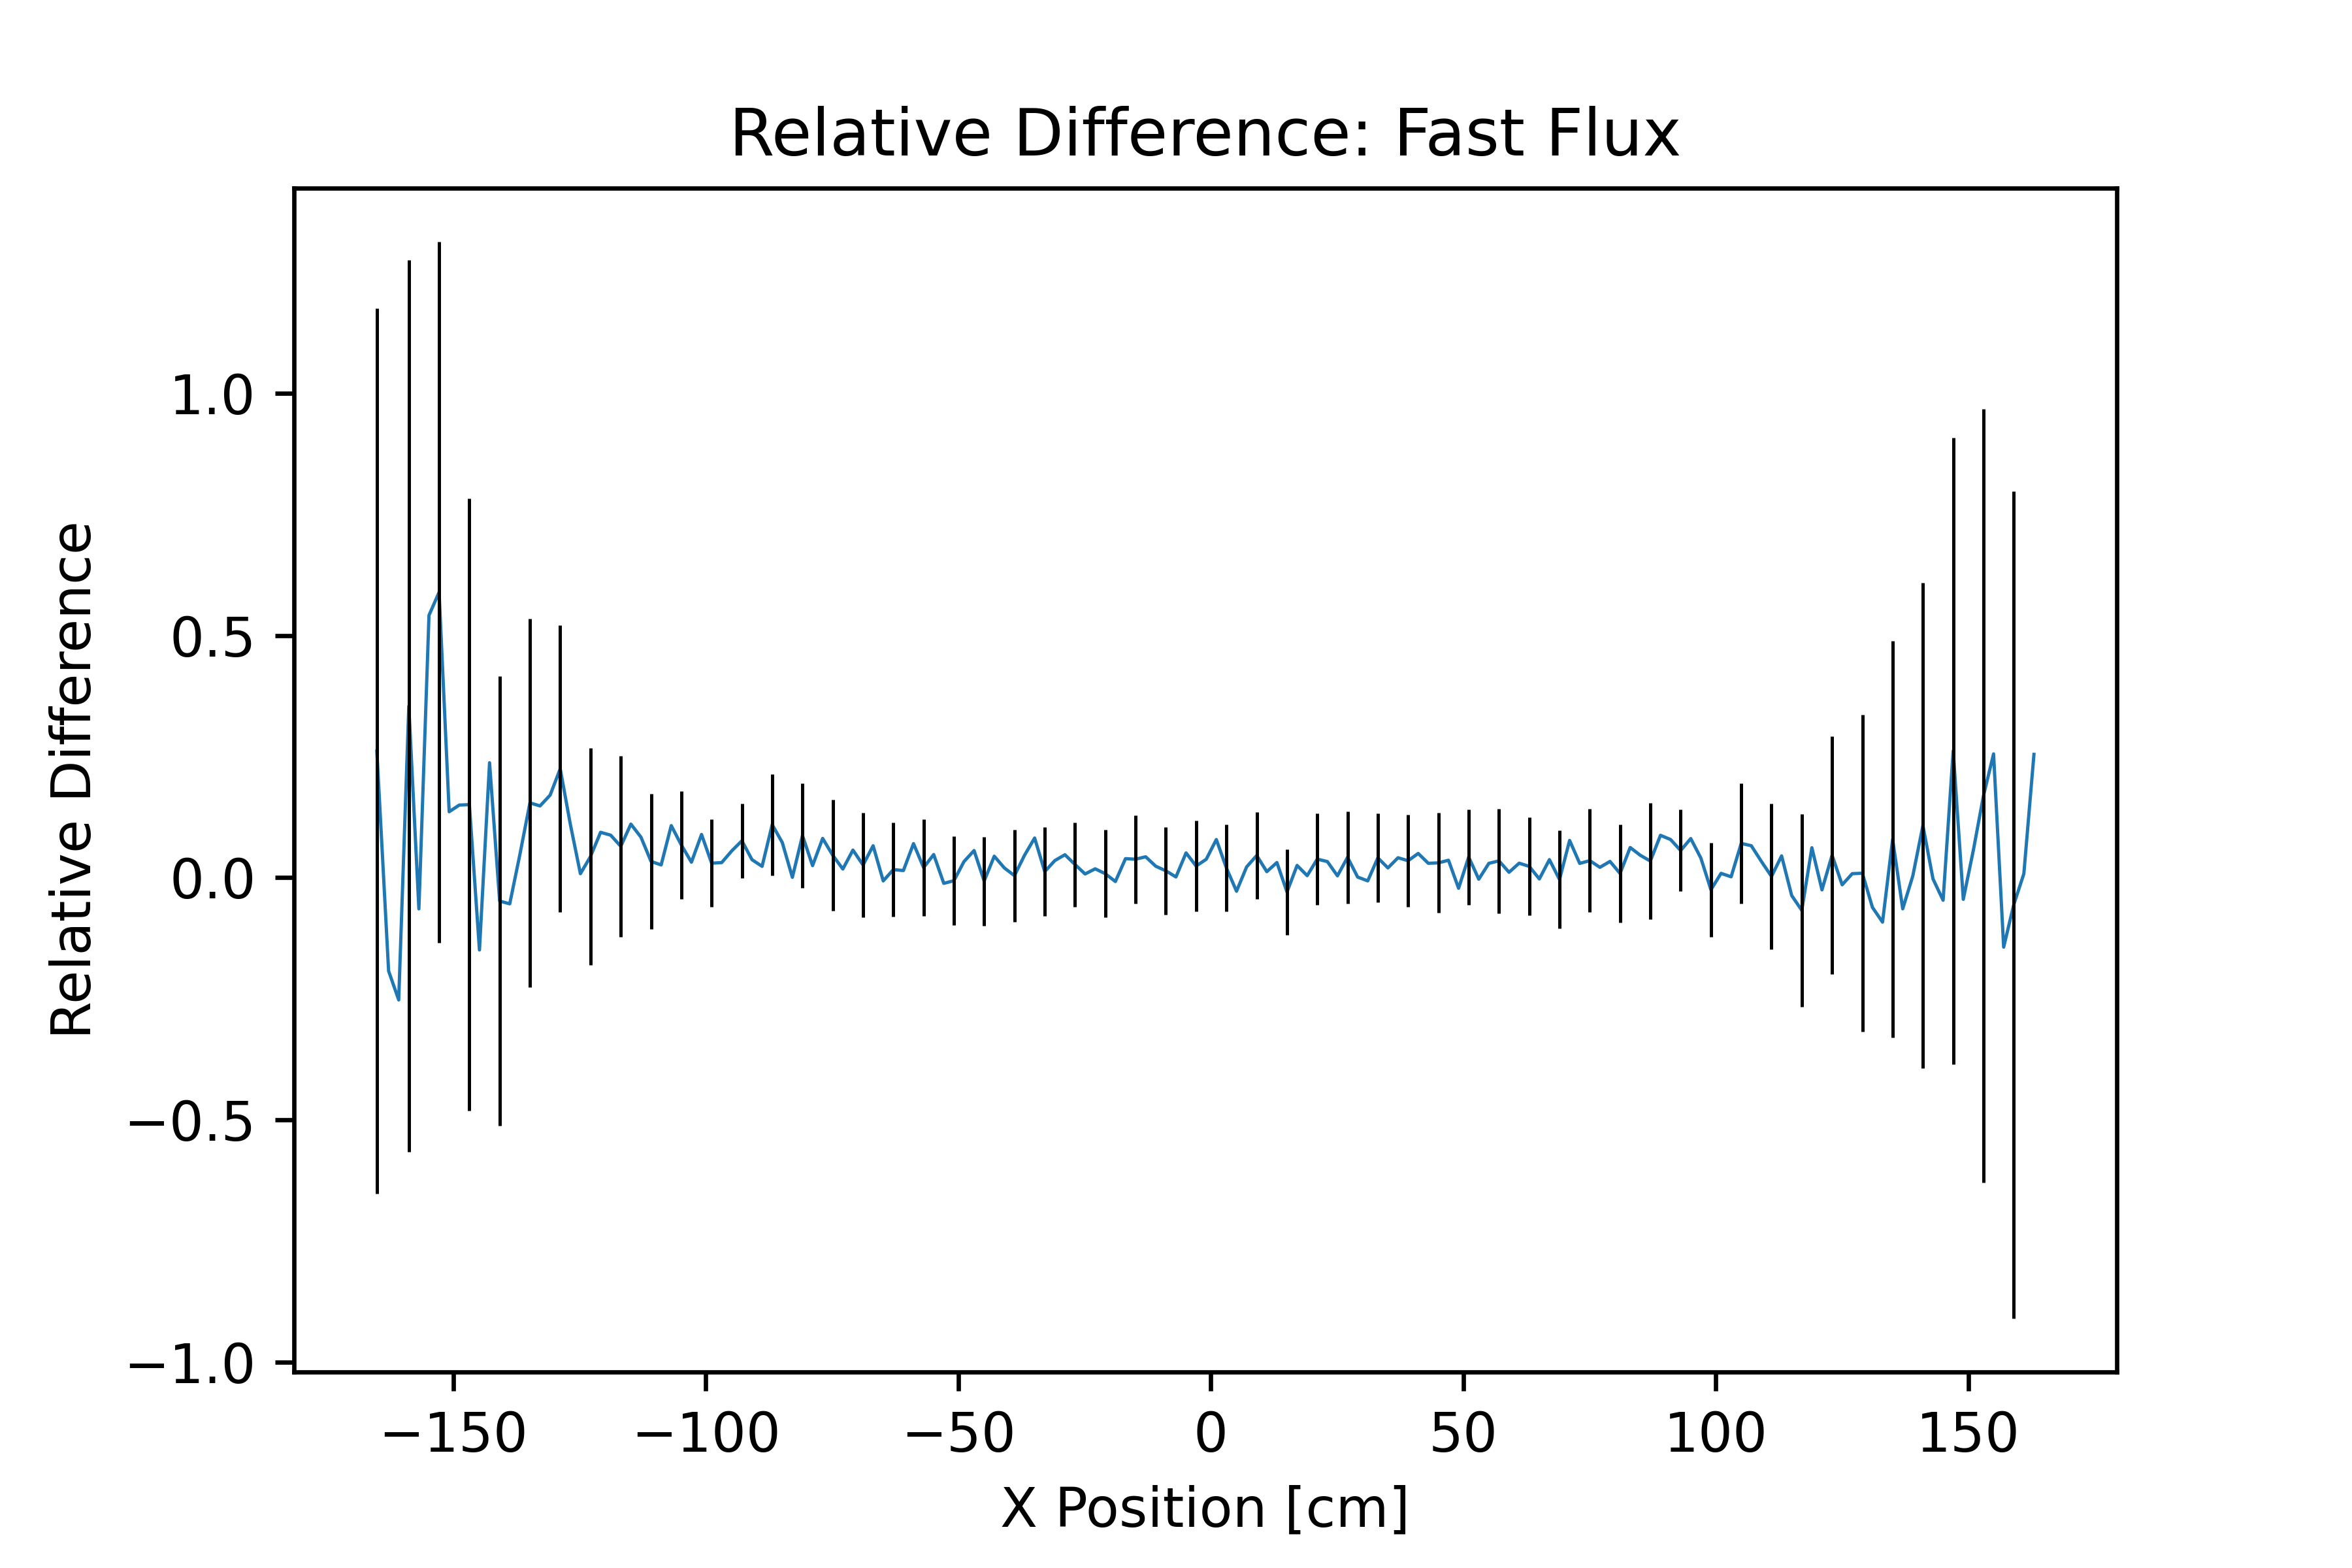
\includegraphics[width=0.9\linewidth]{figures/reldiff_fast_flux.png}
  \caption{Fast Flux}
  \label{fig:diff-fast}
\end{subfigure}

%
\caption[]{(cont.)}
\label{fig:diff-flux}
\end{figure}

The relative difference in the thermal flux is generally between $\pm 10\%$ for the entire span of the reactor.  However, once one accounts for error, it is entirely possible that these differences are wholly accounted for with error alone.  The magnitude of the error is fairly constant --- except at the edges, where it is much larger.  For the fast flux spectrum, the active core region containing the fuel pebbles has a range of $\pm 10-20\%$ relative difference, which is once again accounted for by error.  The error on the outer edges in the fast flux plot is much greater than that in the thermal flux, but this is to be expected --- as said before, the reflector causes significant thermalization of neutrons entering it, and this means that there are fewer fast neutrons in the reflector to contribute to tallies.  For both the thermal and fast fluxes, the value of the relative difference tends to oscillate from one data point to the next.  Additionally, the thermal flux's relative difference has two small peaks, each corresponding with the reflector region.  These peaks, as shown before, coincide with the actual peaks in the thermal flux ~10 cm into the reflector.  This is in contrast to the fast flux relative difference profile, which, although it oscillates like the thermal flux, is generally a flat line, and does \emph{not} feature the same center peak that the fast flux does.

For both the thermal and fast flux profiles, relative difference worsens on the outermost edges.  Overall, Figures \ref{fig:diff-therm} and \ref{fig:diff-fast} suggest that the homogenized simulation is slightly over-predicting the magnitude of the flux when compared to the heterogenized core; however, given the size of the error, these differences do not exist with certainty.


\begin{figure}[H]
\centering
%
\begin{subfigure}{0.95\textwidth}
  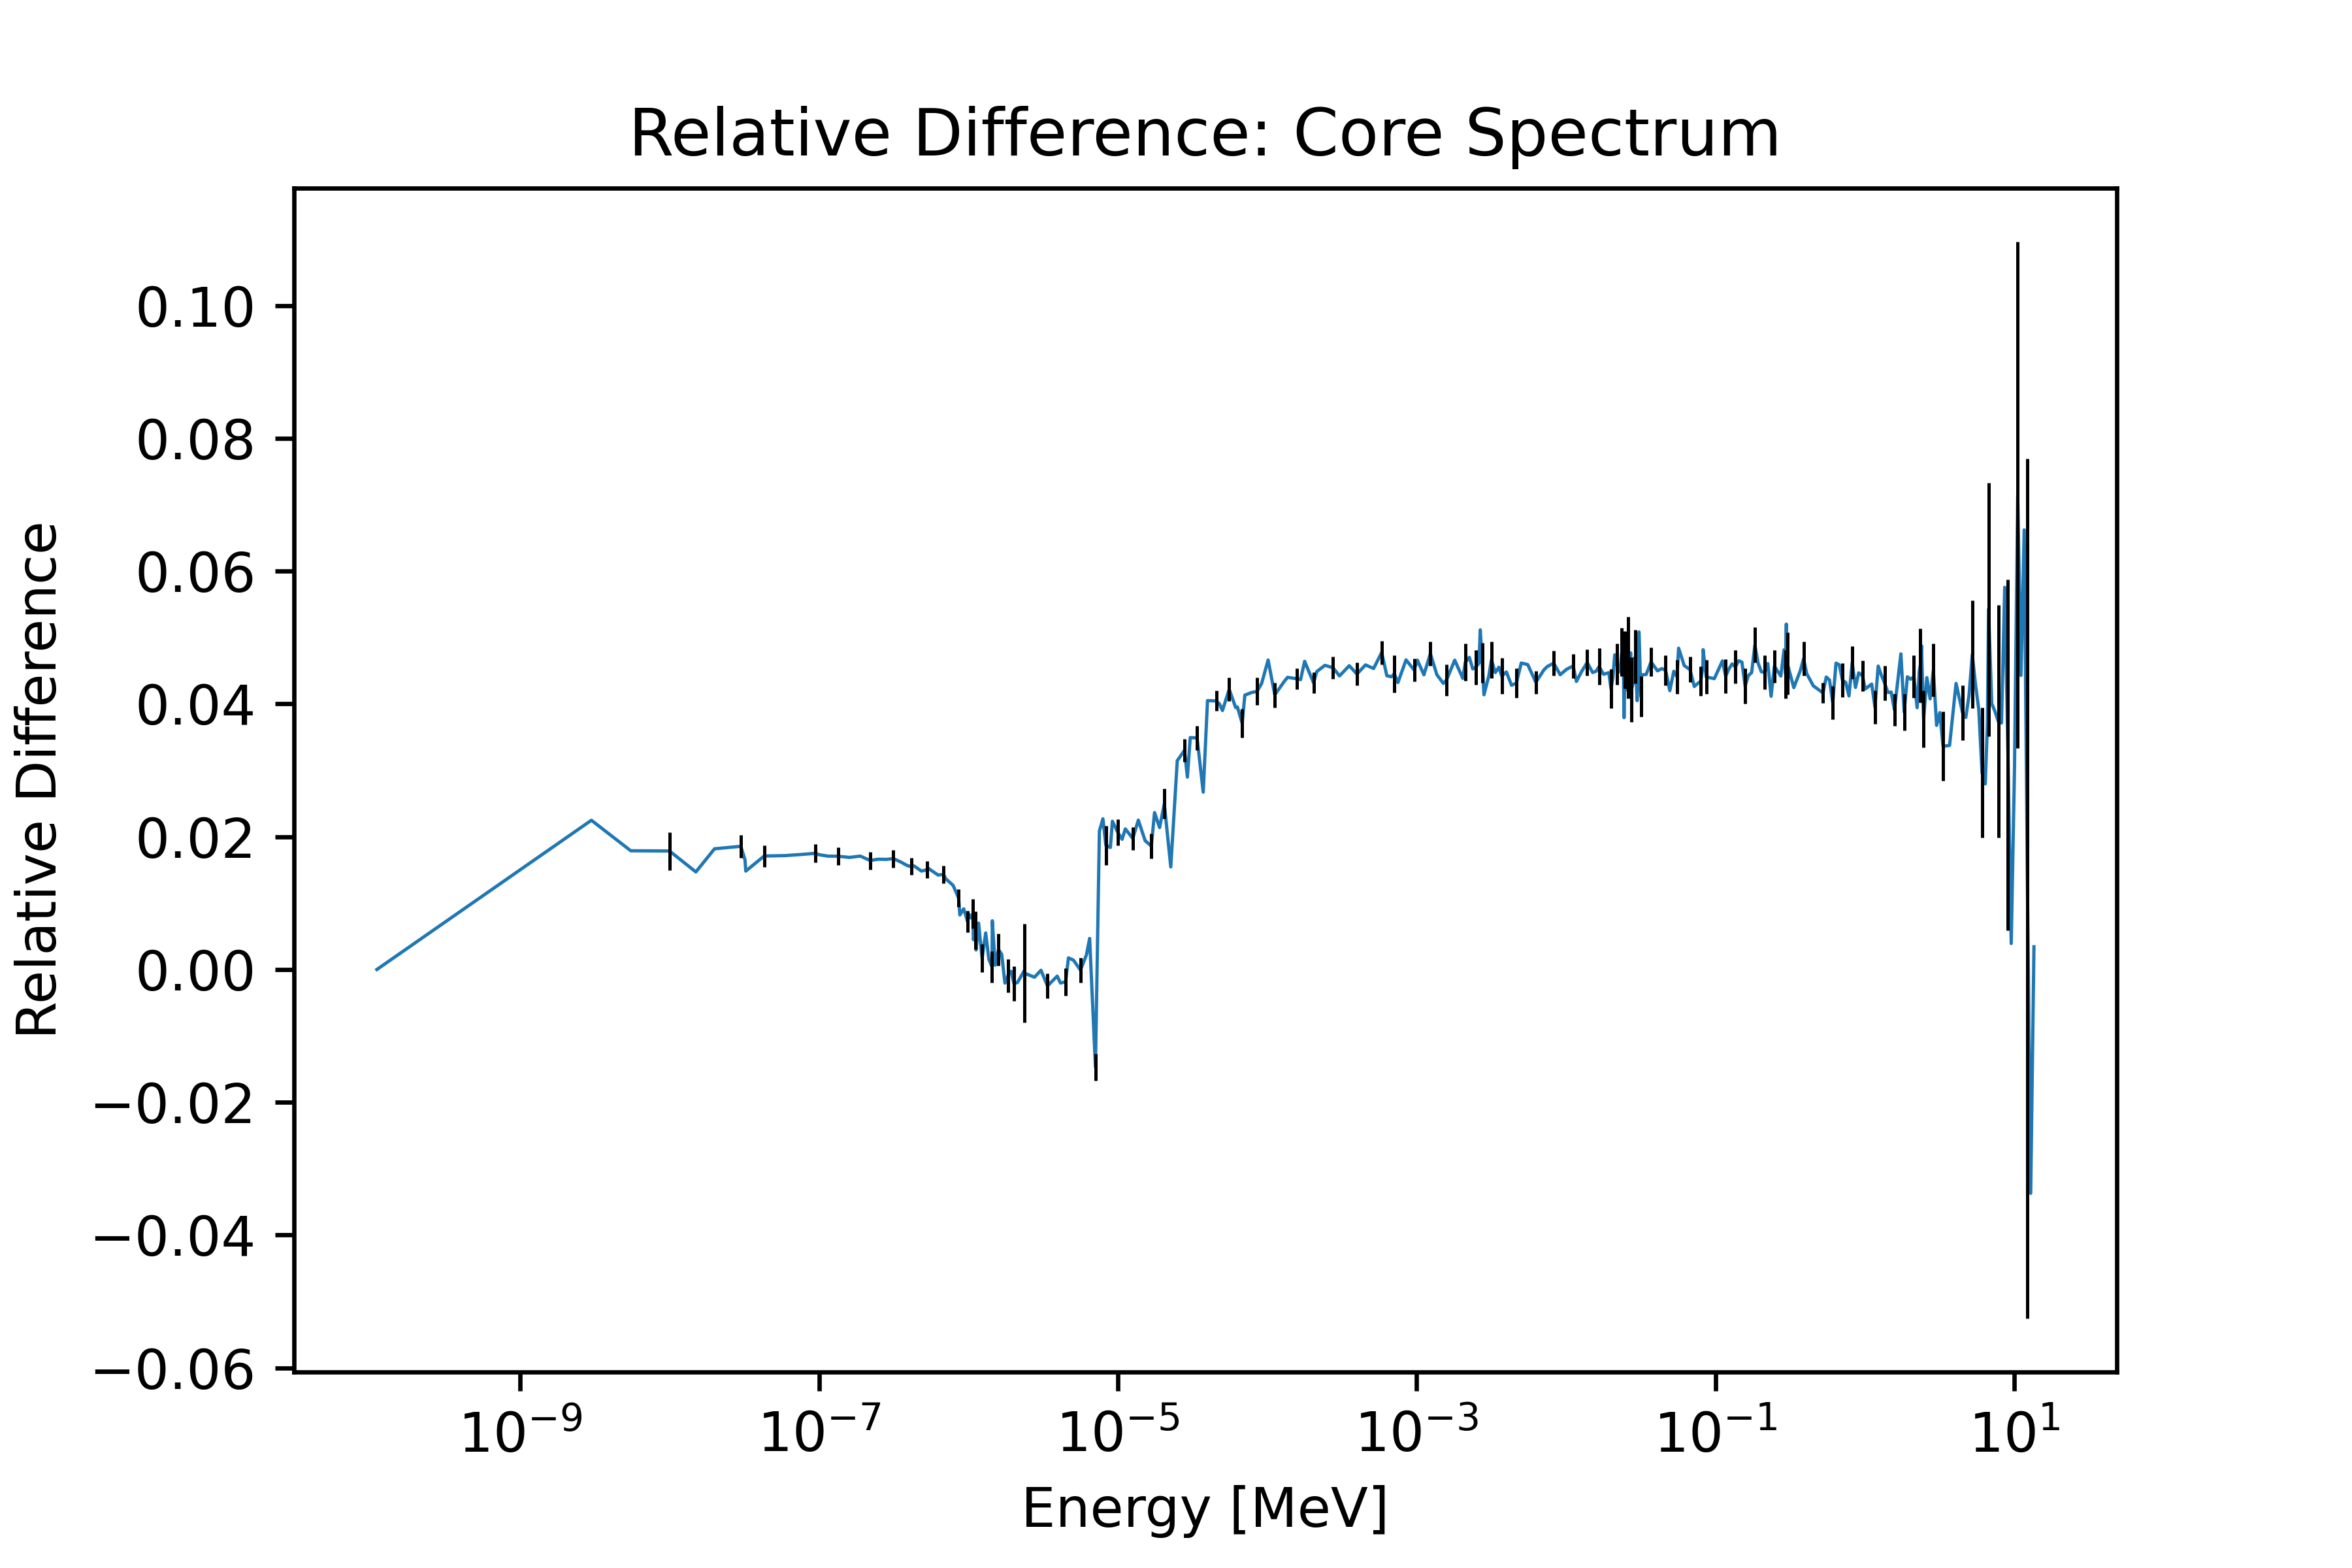
\includegraphics[width=0.95\linewidth]{figures/reldiff_core_spec_er}
  \caption{Core}
  \label{fig:diff-core}
\end{subfigure}%


\begin{subfigure}{0.95\textwidth}
  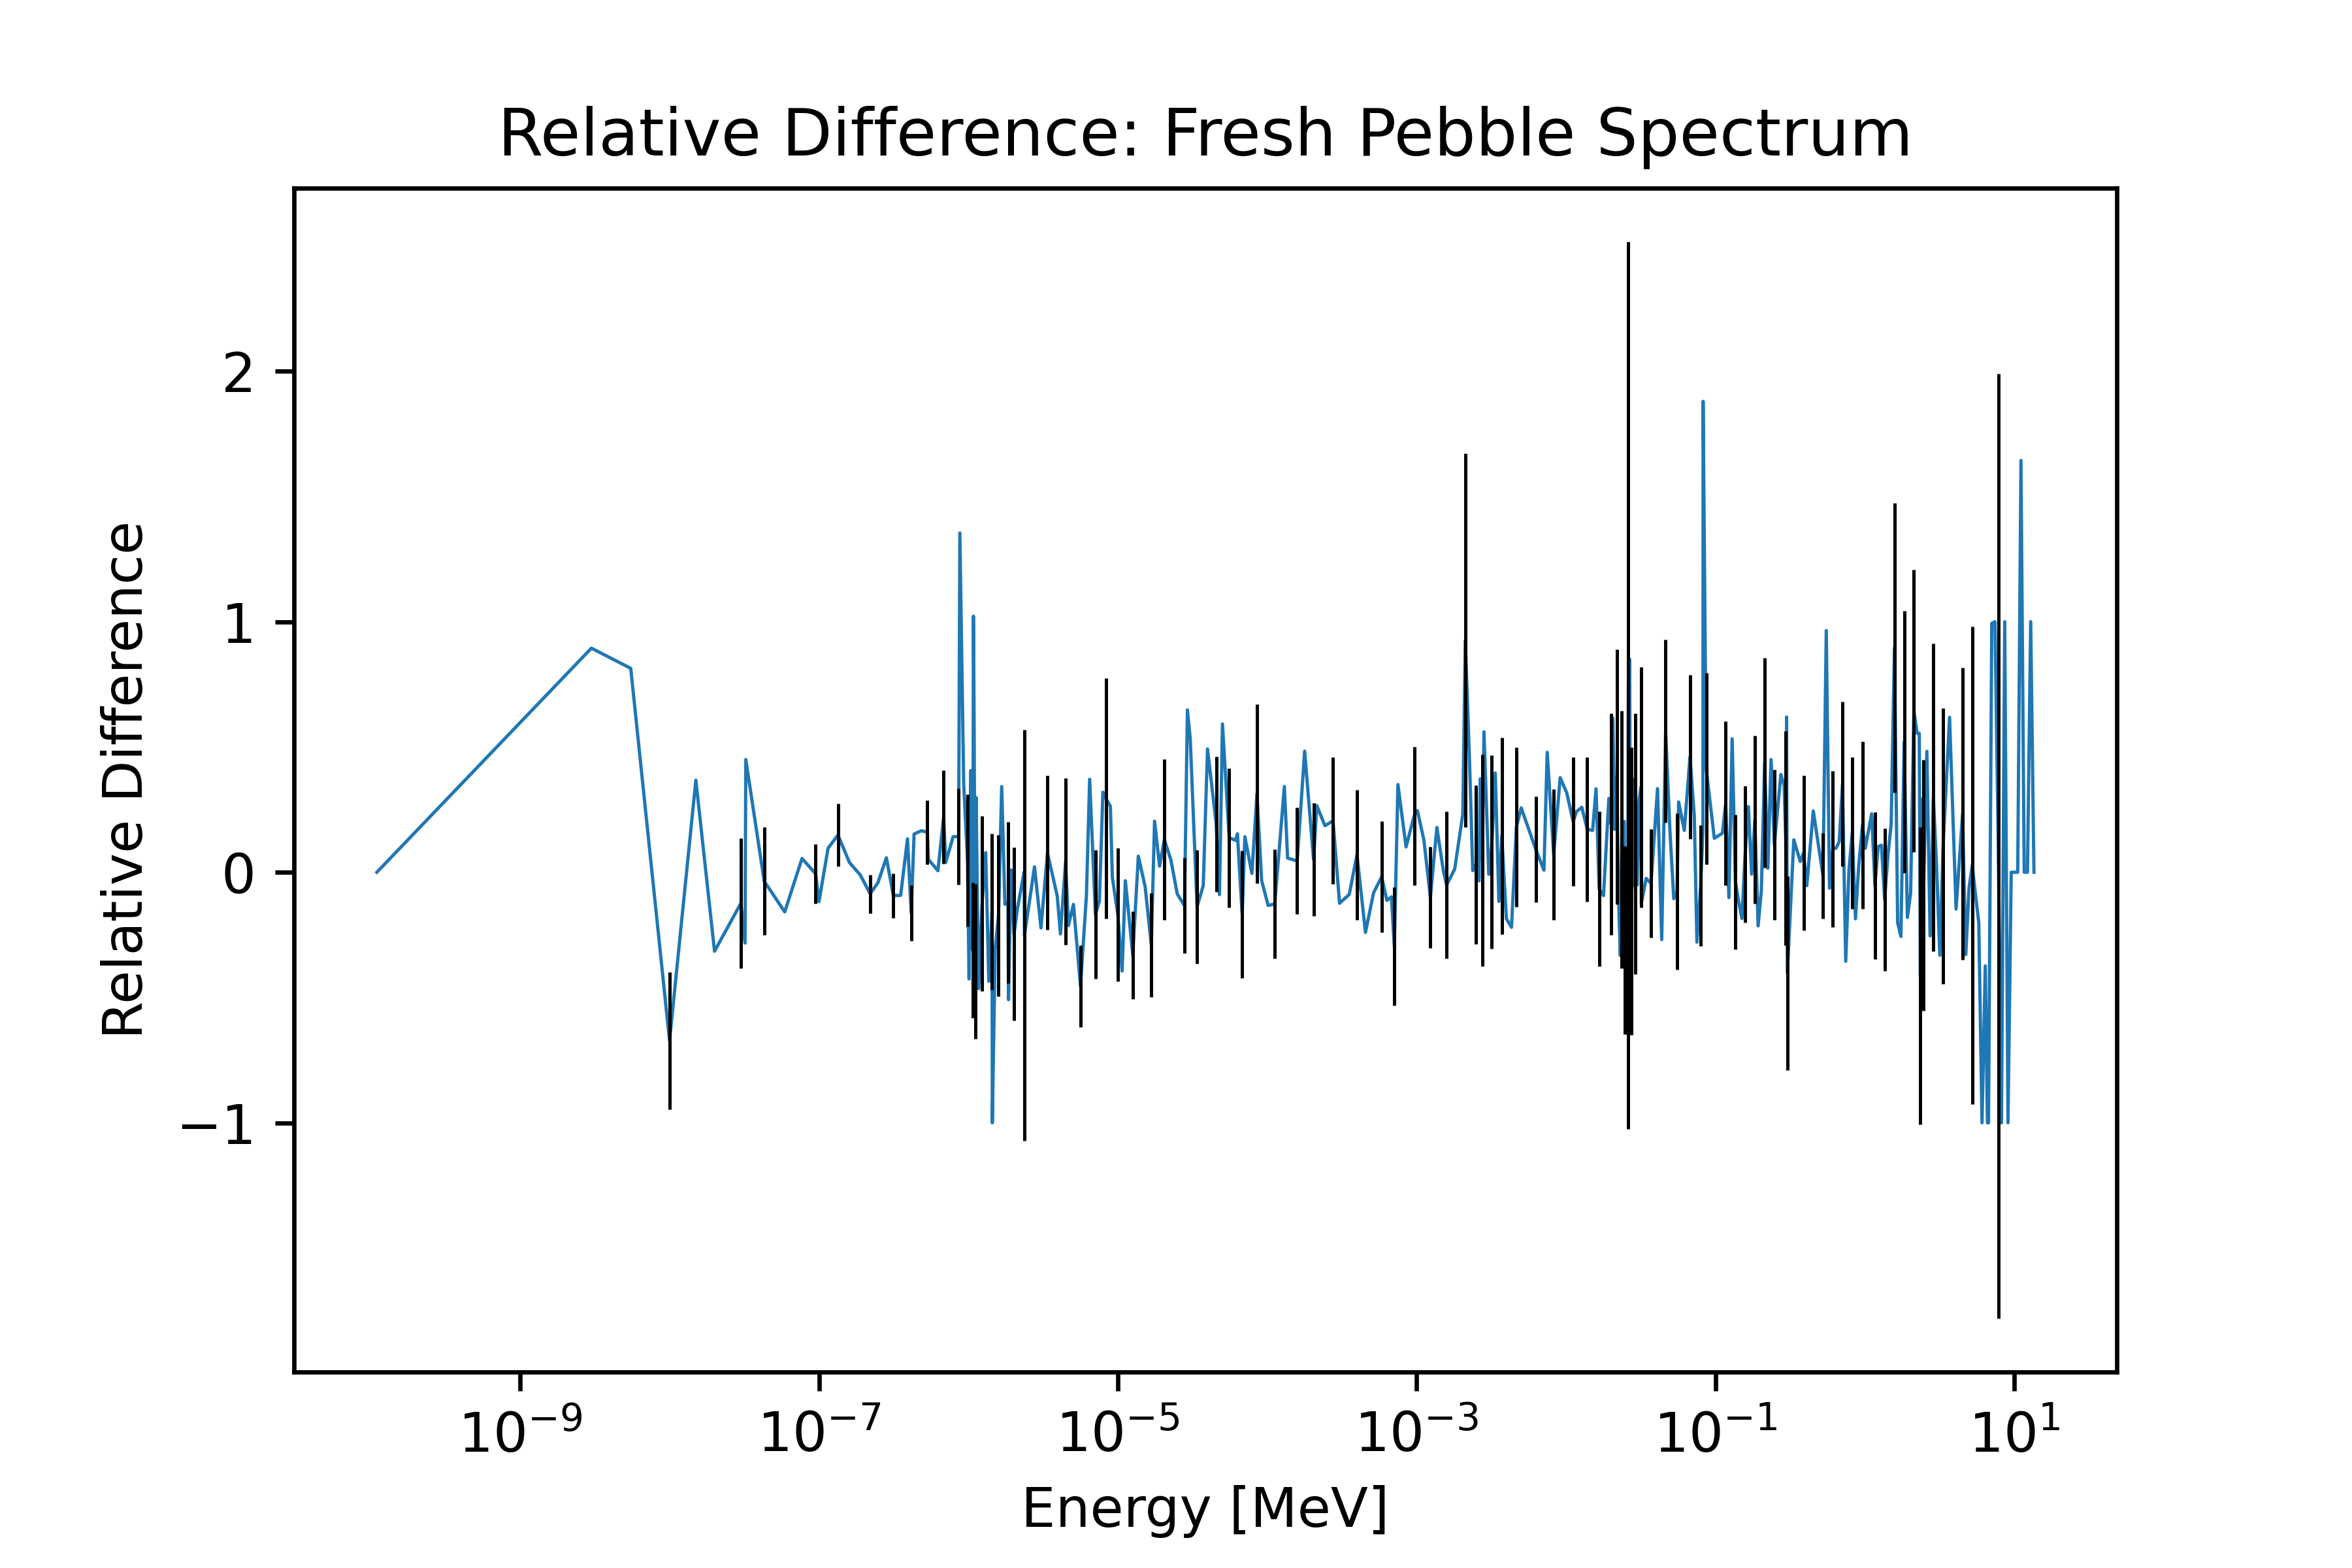
\includegraphics[width=0.95\linewidth]{figures/reldiff_fresh_spec_er}
  \caption{Fresh Pebble}
  \label{fig:diff-fresh}
\end{subfigure}%

\caption{Relative Difference in Lethargy Adjusted Neutron Flux Energy Spectra Between Cores using Homogenized and Heterogenized Pebbles}
\end{figure}

\begin{figure}[H]\ContinuedFloat
\centering

\begin{subfigure}{0.95\textwidth}
  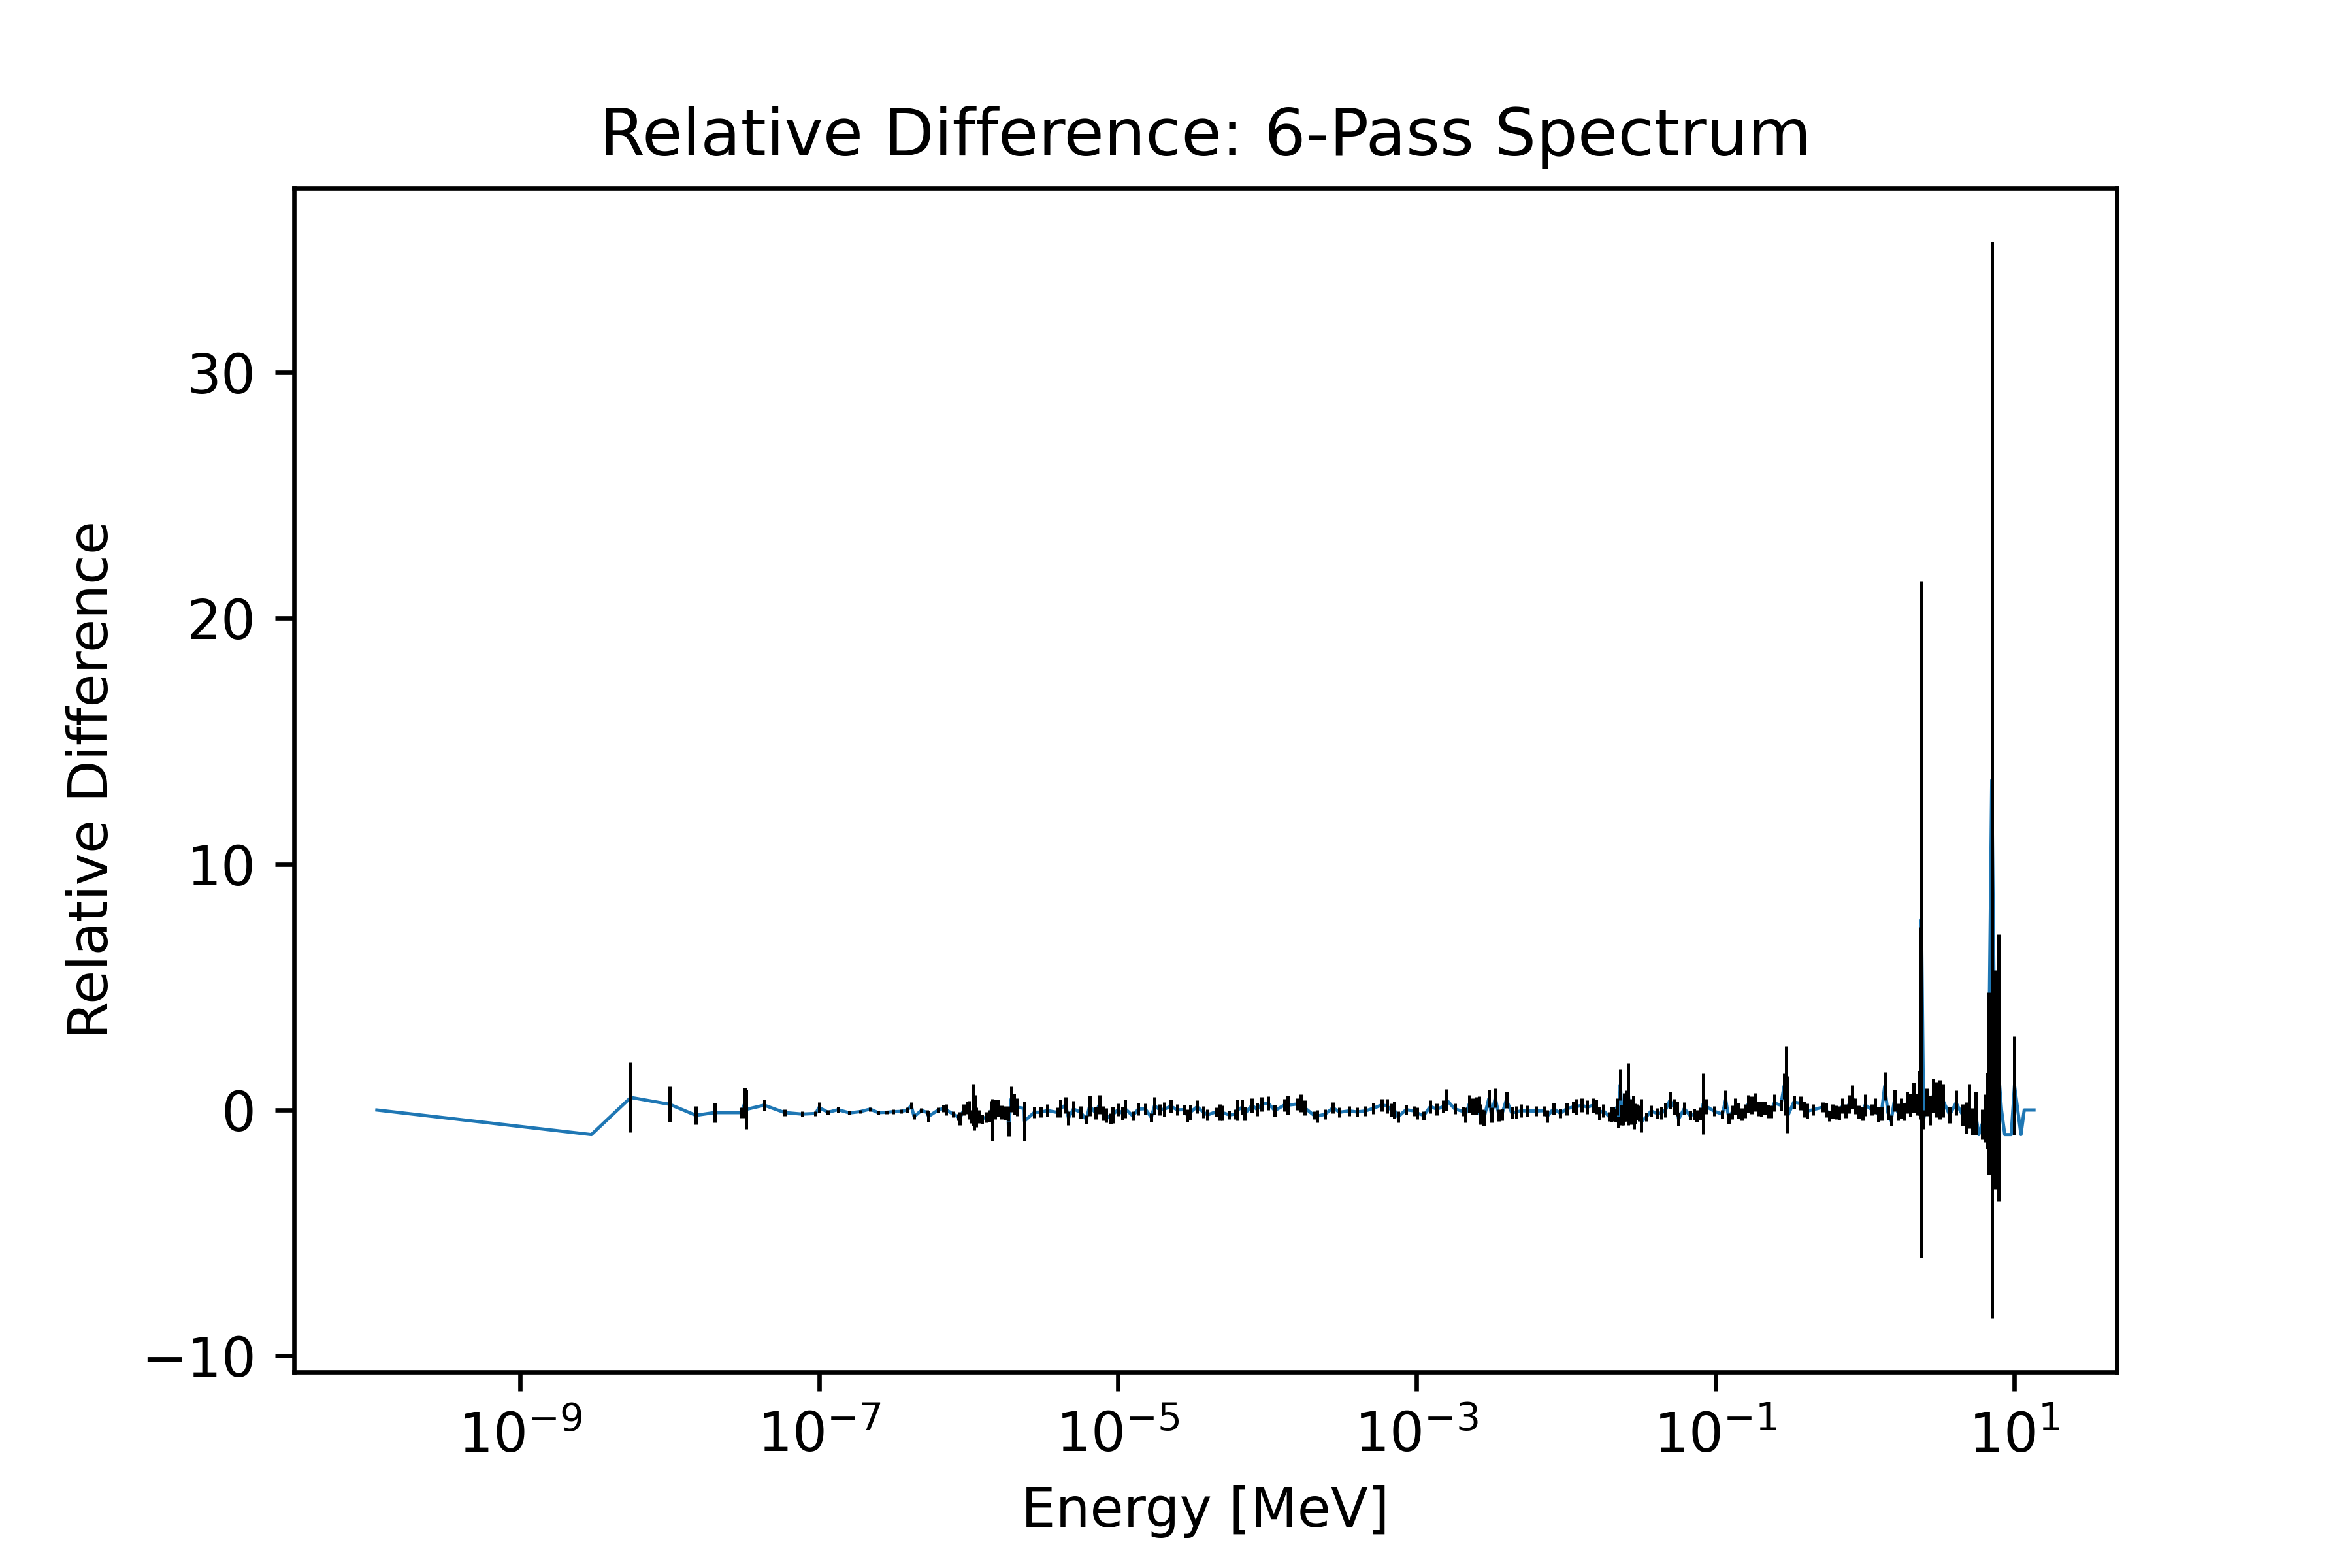
\includegraphics[width=0.95\linewidth]{figures/reldiff_six_spec_er}
  \caption{Six-Pass Pebble}
  \label{fig:diff-six}
\end{subfigure}%


\begin{subfigure}{0.95\textwidth}
  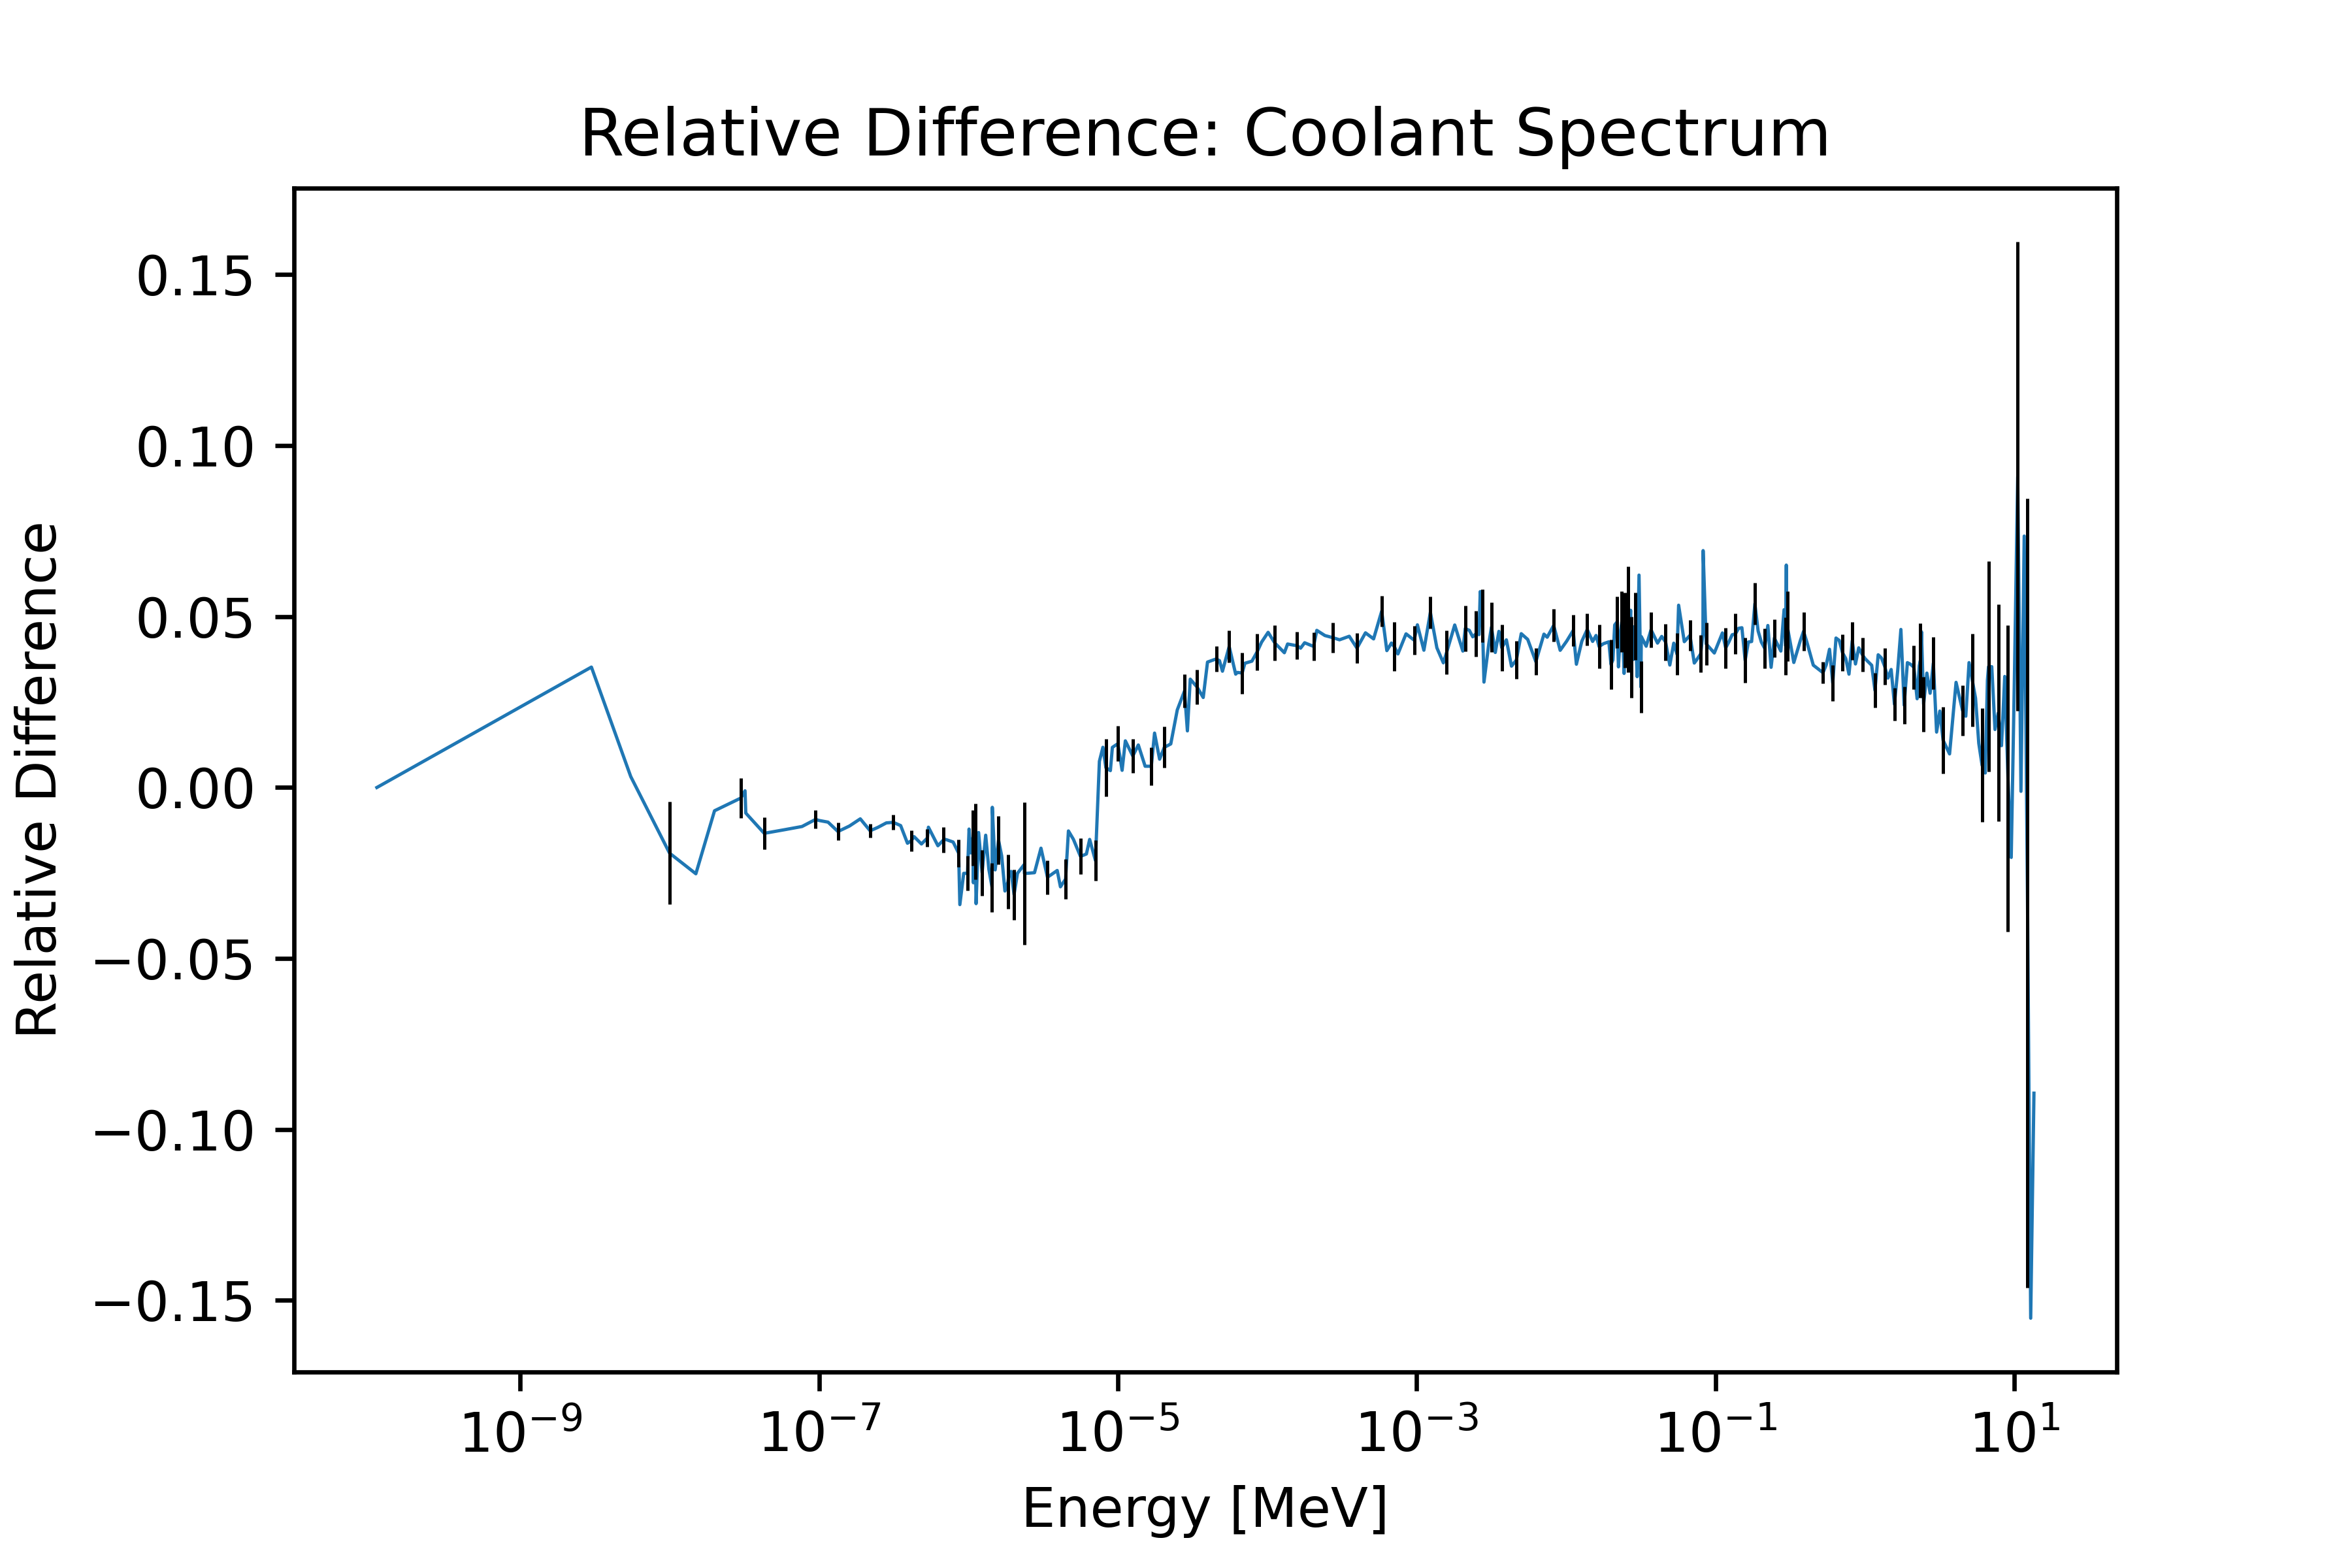
\includegraphics[width=0.95\linewidth]{figures/reldiff_cool_spec_er}
  \caption{Coolant}
  \label{fig:diff-cool}
\end{subfigure}%

\caption[]{(cont.)}
\end{figure}

\begin{figure}[H]\ContinuedFloat
\centering

\begin{subfigure}{0.95\textwidth}
  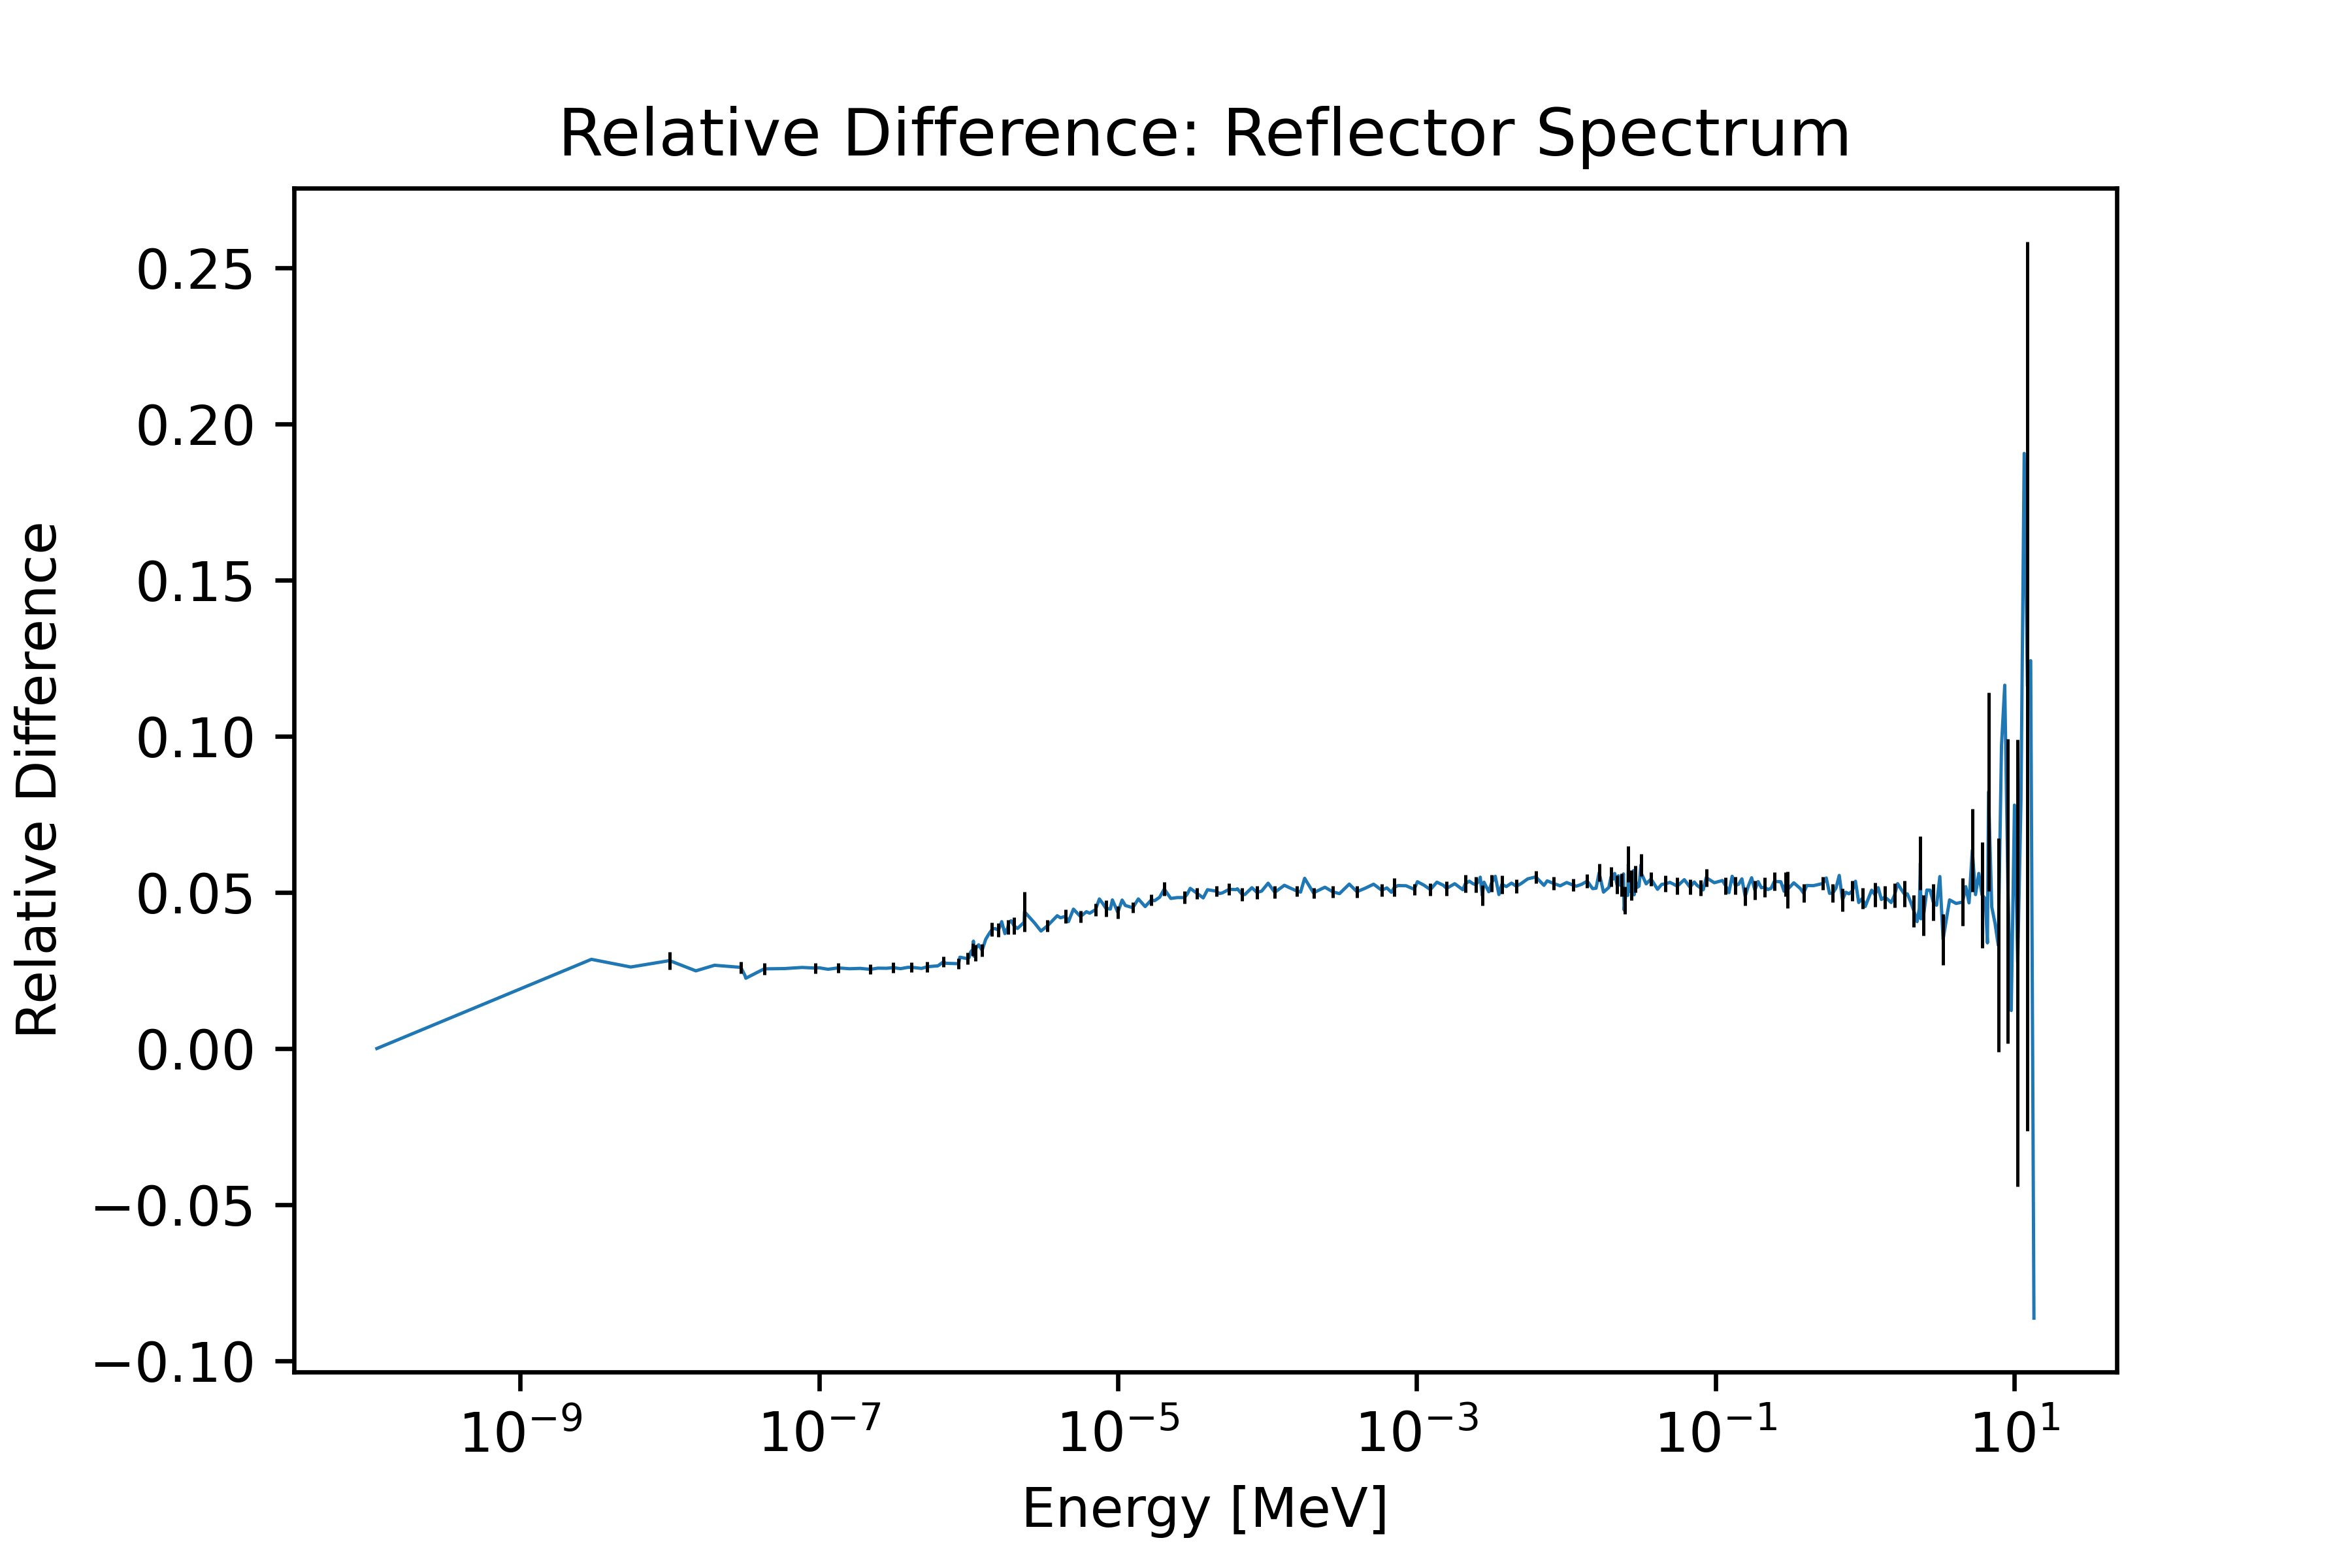
\includegraphics[width=0.95\linewidth]{figures/reldiff_reflec_spec_er}
  \caption{Reflector}
  \label{fig:diff-reflec}
\end{subfigure}%

\caption[]{(cont.)}
\label{fig:diff-spec}
\end{figure}

Figure \ref{fig:diff-spec} shows the relative difference in the core, reflector, coolant, and a fresh and six-pass pebble. For all relative difference images in the spectra, a maximum energy cutoff of 13.499 MeV was applied, as data points after this are too inaccurate (due to the low number of tallies in the spectra being compared) and tend to hide the trends in the lower energy ranges.  Overall, the homogenized model is over-predicting the thermal peak compared with the heterogeneous model in the core spectra by 5\%.  Around $10\times10^{-06}$ MeV, at an energy just above the thermal peak, the two spectra agree before diverging again, this time with a slightly greater disagreement.  Unlike Figure \ref{fig:diff-flux}, considering only error leaves the relative differences seen in Figure \ref{fig:diff-spec} unaccounted for (with the exception of the highest neutron energy ranges, and the pebble spectra, which have higher uncertainty).

The pebble spectra in \ref{fig:diff-fresh} and \ref{fig:diff-six} have a much greater range of relative difference (greater than 1.0, sometimes spiking to factors of 10+).  However, given the wild oscillations and higher error, it is difficult to say with certainty that any of these peaks are "real", and not simply due to error.  Future work could consider using a multi-pebble detector to further resolve these differences.  This is discussed in \autoref{conc}. 

The coolant and core spectra likely provided a better understanding of the effect of homogenization on neutron energy spectra. The coolant spectra in \ref{fig:diff-cool} differed after the thermal peak in a magnitude and shape matching the differences in core spectra in \ref{fig:diff-core}, showing that the homogeneous model is over-predicting the magnitude of the faster neutron energy range by around 5\%.  Unlike the core, however, the coolant has much closer agreement at lower energy levels, including at the thermal peak.  The reflector shows a slight over estimation for the homogeneous spectra, which is consistent for all but the highest energy levels (where low tally scores in the compared spectra's detectors may be the cause).



\section{Shuffling and Symmetry Tests}
Two additional studies look at the effects of assuming a one-sixth core symmetry, and the effects of changing the fuel composition in each pebble, effectively shuffling the pebbles without re-generating their location.  All tests use the homogenized pebble assumption as a base.

\subsection{Effects of Symmetry Assumption}
\label{res-sym}

Overall, the effects of using a one-sixth core symmetry were minimal.  \ref{table:slicesens} shows the effect of symmetry assumptions on the $k_{eff}$ and current, and compares them to the control model.  In Table \ref{table:slicesens} the relative difference between $k_{eff}$ and $J^+$ are calculated between the value provided in the table, and the same parameter in the Sangamon20 control model (see \autoref{res-control}).



\begin{table}[H]
\centering
\caption{Symmetry Run Results Summary}
 \begin{tabularx}{0.7\textwidth}{c  c  c  c  c}
 	\hline
 	Run & $k_{eff}$ & $k_{eff}$ $\% \Delta$ & $J^+$  $[\frac{n}{cm^2s}]$ & $J^+$ $\% \Delta$  \\
 	\hline
 	Run 1 & 1.03990 $\pm$ 0.00055 & 0.0836$\%$ & $5.921\times10^{11}$ $\pm$ $8.704\times10^{08}$ & 0.626$\%$ \\
 	Run 2 & 1.03979 $\pm$ 0.00050 & 0.0942$\%$ & $5.884\times10^{11}$ $\pm$ $8.296\times10^{08}$ & 0.010$\%$ \\
 	Run 3 & 1.04150 $\pm$ 0.00054 & 0.0701$\%$ & $5.908\times10^{11}$ $\pm$ $7.444\times10^{08}$ & 0.392$\%$ \\
 	Run 4 & 1.03927 $\pm$ 0.00057 & 0.144$\%$ & $5.910\times10^{11}$ $\pm$ $8.687\times10^{08}$ & 0.425$\%$ \\
 	Run 5 & 1.04154 $\pm$ 0.00054 & 0.0740$\%$ & $5.884\times10^{11}$ $\pm$ $8.885\times10^{08}$ & 0.010$\%$ \\
 	Run 6 & 1.04047 $\pm$ 0.00050 & 0.0288$\%$ & $5.888\times10^{11}$ $\pm$ $8.478\times10^{08}$ & 0.057$\%$ \\
 	\hline

 \end{tabularx}
\label{table:slicesens}
\end{table}

Figure \ref{fig:0-60} provides cross-sections of the geometry, and fission rate/thermal flux meshes for a one-sixth core symmetry test, in this case Run 1.  The fission rate mesh naturally exhibits a six-part repeating pattern, and still shows the banding patterns on the outer edges.   Other runs are not shown due to similar features, but can be found in \autoref{app-sym}


\begin{figure}[h!]
\centering

\begin{subfigure}{0.45\textwidth}
  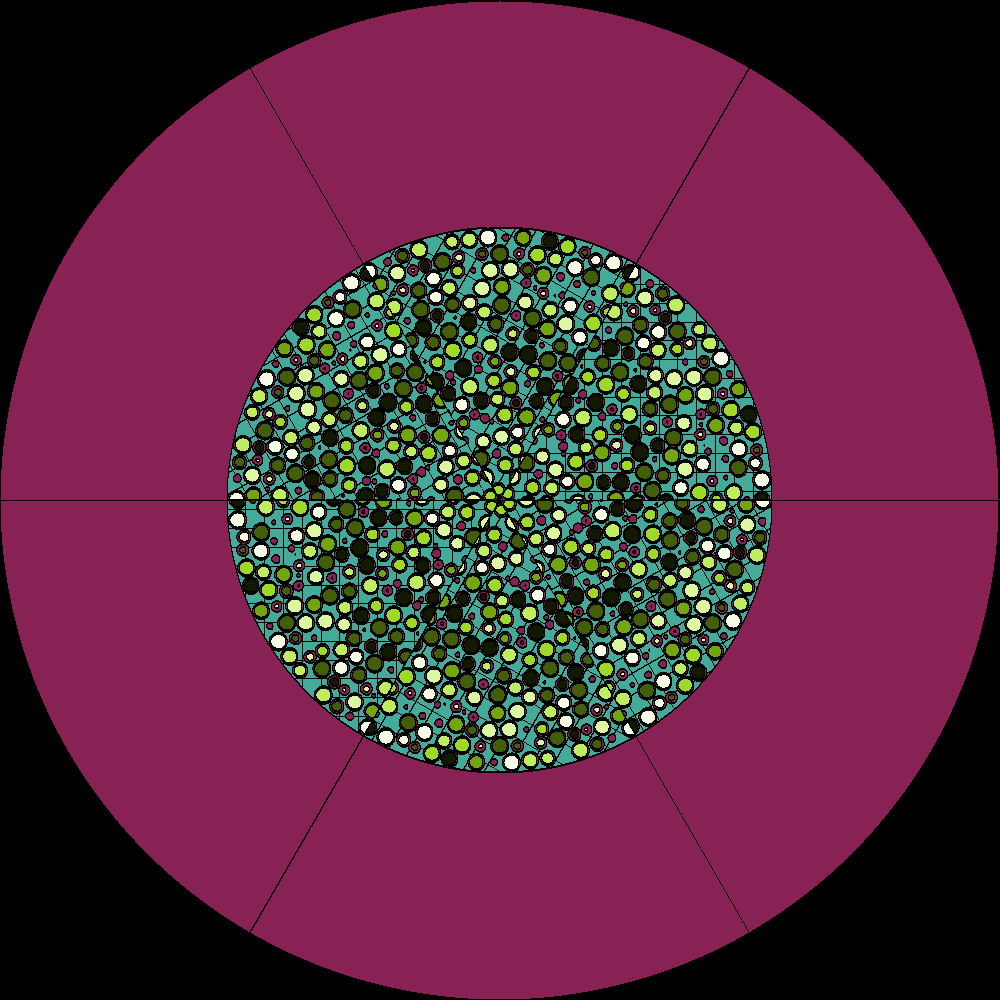
\includegraphics[width=0.95\linewidth]{figures/0-60/0-60-r}
  \caption{Radial Cross Section at y=0}
  \label{fig:0-60-r}
\end{subfigure}%
%
\begin{subfigure}{0.45\textwidth}
  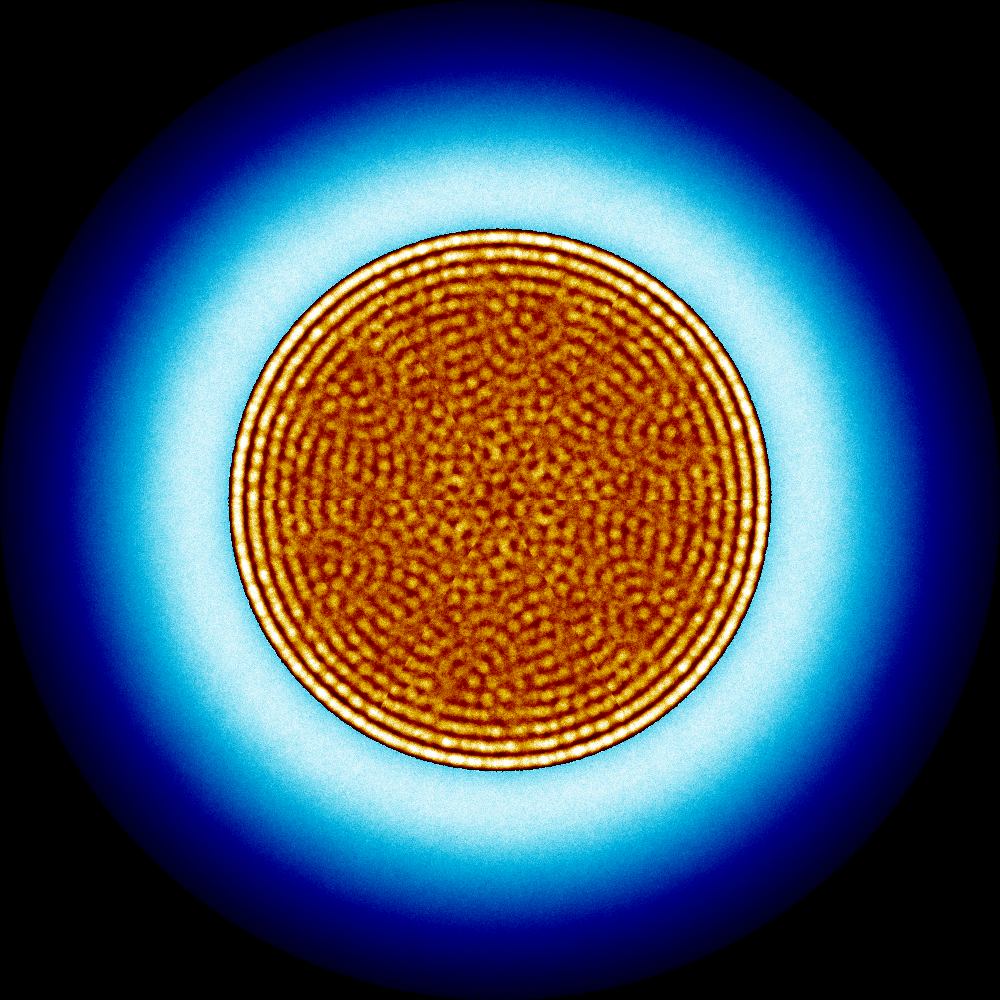
\includegraphics[width=0.95\linewidth]{figures/0-60/0-60-rm}
  \caption{Radial Mesh}
  \label{fig:0-60-rm}
\end{subfigure}

\begin{subfigure}{0.45\textwidth}
  \includegraphics[width=0.95\linewidth]{figures/0-60/0-60-v}
  \caption{Axial Cross Section at z=0 }
  \label{fig:0-60-v}
\end{subfigure}
%
\begin{subfigure}{0.45\textwidth}
  \includegraphics[width=0.95\linewidth]{figures/0-60/0-60-vm}
  \caption{Axial Mesh}
  \label{fig:0-60-vm}
\end{subfigure}
%
\caption{Sensitivity Analysis: $0^{\circ}$ - $60^{\circ}$}
\label{fig:0-60}
\end{figure}
One point of interest is the degree to which the region from 0 to 60 degrees matches the same region in the control fission rate mesh.  An image subtraction program generated Figure \ref{fig:htgr-diff} by subtracting the radial meshes for the control (Figure \ref{fig:controlb}) and first symmetry test (Figure \ref{fig:0-60-rm}).  For a more detailed description of its use, please refer to \autoref{app-rgb}.  Figure \ref{fig:htgr-diff} allows us to more clearly observe where differences are strongest between the models.

\begin{figure}[h!]
\centering
\includegraphics[width=0.6\linewidth]{figures/htgr-diff}
\caption{An Image Generated by Subtracting \ref{fig:0-60-rm} from \ref{fig:htgr-diff}.}
\label{fig:htgr-diff}
\end{figure}

Within the region between 0 and 60 degrees, the two meshes are almost identical, pixel for pixel.  While this might be unsurprising in the center of this region, the perfect match towards the edges of it are less so.  As a reminder, the symmetry tests all use a one-sixth symmetry, and a periodic boundary condition, i.e., if a neutron leaves the slice on one side, it re-enters the slice on the other.  In effect, the edges of the 0 to 60 degree slice in the symmetry test are seeing entirely different materials, compared with the control.  The edges in \ref{fig:htgr-diff} are not a gradient, but rather a hard line, which may suggest that with proper mixing nearest-neighbor pebbles have a relatively lesser impact on core parameters.  However, note that Sangamon20 uses only fuel pebbles, and this observation may be false in a reactor design using, for example, absorber pebbles containing something such as boron, or inert pebbles at the edge to protect the reflector.  For the results of Symmetry tests 2 through 6, see \autoref{app-sym}.


\subsection{Effects of Pebble Shuffling}
\label{res-shuff}

The final test on the effects of changes to core modeling is another test of consistency between similar HTGR designs with a different pebble configurations.  Rather than re-generate the pebble locations several times, the 'shuffling' test simply reassigns each pebble with a different fuel composition (creating a new input file).  For example, the pebbles that were once fresh are now first-pass, the first pass pebbles are now second-pass, and so on.  The manual shuffling followed the process outlined in \autoref{meth-sens}, Table \ref{table:shuffle}, and the results of this test are in Table \ref{table:shufsens}.



\begin{table}[H]
\centering
 \begin{tabularx}{0.7\textwidth}{c  c  c  c  c}
 	\hline
 	Run & $k_{eff}$ & $k_{eff}$ $\% \Delta$ & $J^+$  $[\frac{n}{cm^2s}]$ & $J^+$ $\% \Delta$ \\
 	\hline
 	Run 1 & 1.03994 $\pm$ 0.00054 & 0.0797$\%$ & $5.897\times10^{11}$ $\pm$ $8.668\times10^{08}$ & 0.211$\%$ \\
 	Run 2 & 1.03999 $\pm$ 0.00055 & 0.0749$\%$ & $5.902\times10^{11}$ $\pm$ $8.086\times10^{08}$  & 0.295$\%$ \\
 	Run 3 & 1.04002 $\pm$ 0.00053 & 0.0721$\%$ & $5.896\times10^{11}$ $\pm$ $8.490\times10^{08}$ & 0.192$\%$  \\
 	Run 4 & 1.04103 $\pm$ 0.00057 & 0.0249$\%$ & $5.884\times10^{11}$ $\pm$ $9.355\times10^{08}$ & 0.013$\%$ \\
 	Run 5 & 1.03960 $\pm$ 0.00053 & 0.112$\%$ & $5.904\times10^{11}$ $\pm$ $8.443\times10^{08}$ & 0.329$\%$  \\
 	Run 6 & 1.04014 $\pm$ 0.00057 & 0.0605$\%$ & $5.898\times10^{11}$ $\pm$ $7.726\times10^{08}$ & 0.227$\%$ \\
 	\hline

 \end{tabularx}
\caption{Shuffling Run Summary}
\label{table:shufsens}
\end{table}

As with \ref{table:slicesens}, \ref{table:shufsens} shows $k_{eff}$ and the current of each perturbation and compares them to the control.  Overall, much like the symmetry test, re-mixing the pebbles had little effect on overall results.  Likely, provided the pebbles are sufficiently mixed, and no 'pockets' of like pebbles exist, designs that are otherwise identical should provide similar results.  For all geometry cross-sections and thermal flux/fission rate mesh images, and the results of image difference for each run, see \autoref{app-shuf}.